% Options for packages loaded elsewhere
\PassOptionsToPackage{unicode}{hyperref}
\PassOptionsToPackage{hyphens}{url}
%
\documentclass[
]{book}
\usepackage{amsmath,amssymb}
\usepackage{lmodern}
\usepackage{iftex}
\ifPDFTeX
  \usepackage[T1]{fontenc}
  \usepackage[utf8]{inputenc}
  \usepackage{textcomp} % provide euro and other symbols
\else % if luatex or xetex
  \usepackage{unicode-math}
  \defaultfontfeatures{Scale=MatchLowercase}
  \defaultfontfeatures[\rmfamily]{Ligatures=TeX,Scale=1}
\fi
% Use upquote if available, for straight quotes in verbatim environments
\IfFileExists{upquote.sty}{\usepackage{upquote}}{}
\IfFileExists{microtype.sty}{% use microtype if available
  \usepackage[]{microtype}
  \UseMicrotypeSet[protrusion]{basicmath} % disable protrusion for tt fonts
}{}
\makeatletter
\@ifundefined{KOMAClassName}{% if non-KOMA class
  \IfFileExists{parskip.sty}{%
    \usepackage{parskip}
  }{% else
    \setlength{\parindent}{0pt}
    \setlength{\parskip}{6pt plus 2pt minus 1pt}}
}{% if KOMA class
  \KOMAoptions{parskip=half}}
\makeatother
\usepackage{xcolor}
\usepackage{longtable,booktabs,array}
\usepackage{calc} % for calculating minipage widths
% Correct order of tables after \paragraph or \subparagraph
\usepackage{etoolbox}
\makeatletter
\patchcmd\longtable{\par}{\if@noskipsec\mbox{}\fi\par}{}{}
\makeatother
% Allow footnotes in longtable head/foot
\IfFileExists{footnotehyper.sty}{\usepackage{footnotehyper}}{\usepackage{footnote}}
\makesavenoteenv{longtable}
\usepackage{graphicx}
\makeatletter
\def\maxwidth{\ifdim\Gin@nat@width>\linewidth\linewidth\else\Gin@nat@width\fi}
\def\maxheight{\ifdim\Gin@nat@height>\textheight\textheight\else\Gin@nat@height\fi}
\makeatother
% Scale images if necessary, so that they will not overflow the page
% margins by default, and it is still possible to overwrite the defaults
% using explicit options in \includegraphics[width, height, ...]{}
\setkeys{Gin}{width=\maxwidth,height=\maxheight,keepaspectratio}
% Set default figure placement to htbp
\makeatletter
\def\fps@figure{htbp}
\makeatother
\setlength{\emergencystretch}{3em} % prevent overfull lines
\providecommand{\tightlist}{%
  \setlength{\itemsep}{0pt}\setlength{\parskip}{0pt}}
\setcounter{secnumdepth}{5}
\usepackage{booktabs}
\usepackage{amsthm}
\makeatletter
\def\thm@space@setup{%
  \thm@preskip=8pt plus 2pt minus 4pt
  \thm@postskip=\thm@preskip
}
\makeatother
\ifLuaTeX
  \usepackage{selnolig}  % disable illegal ligatures
\fi
\usepackage[]{natbib}
\bibliographystyle{apalike}
\IfFileExists{bookmark.sty}{\usepackage{bookmark}}{\usepackage{hyperref}}
\IfFileExists{xurl.sty}{\usepackage{xurl}}{} % add URL line breaks if available
\urlstyle{same} % disable monospaced font for URLs
\hypersetup{
  pdftitle={An Introduction to Neuroscience},
  pdfauthor={Robert J Calin-Jageman and others},
  hidelinks,
  pdfcreator={LaTeX via pandoc}}

\title{An Introduction to Neuroscience}
\author{Robert J Calin-Jageman and others}
\date{2022-12-31}

\begin{document}
\maketitle

{
\setcounter{tocdepth}{1}
\tableofcontents
}
\hypertarget{introduction}{%
\chapter{Introduction}\label{introduction}}

This is a free, open-source, peer-reviewed, high-quality Introduction to Neuroscience textbook\ldots{} or it soon will be.

At this stage, I have only Chapter \ref{neurophysiology} (Neurophysiology) posted in draft form. More to come!

\hypertarget{neurophysiology}{%
\chapter{Neurophysiology - by Robert J Calin-Jageman}\label{neurophysiology}}

\hypertarget{neurophysiology-introduction}{%
\section{Introduction}\label{neurophysiology-introduction}}

Mary is visiting the office of Dr.~Alfredo Quinones-Hinojosa, a neuroscientist, physician, and neurosurgeon who is known affectionately by his patients as ``Dr.~Q''. Unfortunately, it is not a happy visit---Mary has been diagnosed with a glioma, a tumor caused by runaway cell division among the glial cells in her brain. Her first sign that something was wrong was a seizure, an episode of tremoring and muscle rigidity that left Mary exhausted and frightened. Now brain scans have revealed a glioma.

Mary is worried. Dr.~Q patiently walks her through her prognosis, explaining how his team can conduct surgery to remove the glioma. ``Will that stop the seizures?'' Mary asks. ``Maybe'' says Dr.~Q. But he warns that in almost 30\% of cases, seizures persist even after a glioma is removed. How can that be? Why would a tumor cause seizures in the first place? And if the tumor is removed, shouldn't the seizures go away? These are some of the medical mysteries Dr.~Q's research team is trying to solve. In fact, Mary decides to donate tissue from her removed tumor to be studied, and with that tissue and samples from other patients Dr.~Q's team uncover something remarkable: compared to glioma patients who do not suffer seizures, those with seizures show increased expression of the mRNA for a specific protein, VGLUT1 (Feyissa et al., 2021). VLGUT1 acts to help load the excitatory transmitter glutamate into vesicles to be released. This finding inspires Dr.~Q's team to formulate a new hypothesis: that excess VGLUT1 causes runaway excitation, explaining why some gliomas lead to seizures. There's still lots of work to do to test this hypothesis, but the cutting edge medicine and research of Dr.~Q and his team reflect an emerging theme in our understanding of the nervous systems: The smooth functioning of neural circuits reflects an incredible ballet amongst protein machines working within each of our 86 billion neurons. The environment we live in can reshape which proteins are expressed and how, with profound implications for the functions of the brain.

In this chapter we'll explore neural communication. We'll see that neurons are constantly receiving messages from their partners and their outside world---messages that produce excitation, inhibition, or modulation. When a neuron is sufficiently excited, it generates an action potential---an electrical wave that spreads through the neuron, causing it to send its own chemical messages to all of its partners. In this way, neurons can form circuits, sending and integrating information to produce complex patterns of activity that muscles transform into behavior. How are neurons able to detect chemical signals, produce action potentials, and release transmitter? Through an amazing collection of protein machines: pumps that use energy to build up concentration gradients of electrically charged molecules, channels that monitor the neuron's environment and then switch open or closed to generate electrical currents, and a whole complex of machinery for both releasing transmitter to partner neurons and for detecting transmitter released from partner neurons. Let's dive in!

\textbf{References and works cited}

\begin{itemize}
\item
  Feyissa AM, Carrano A, Wang X, Allen M, Ertekin-Taner N, Dickson DW, Jentoft ME, Rosenfeld SS, Tatum WO, Ritaccio AL, Guerrero-Cázares H, Quiñones-Hinojosa A (2021) Analysis of intraoperative human brain tissue transcriptome reveals putative risk genes and altered molecular pathways in glioma-related seizures. Epilepsy Res 173:106618 Available at: \url{https://linkinghub.elsevier.com/retrieve/pii/S0920121121000711}.
\item
  Quiñones-Hinojosa A (2011). \emph{Becoming Dr.~Q: My Journey from Migrant Farm Worker to Brain Surgeon}. University of California Press.
\end{itemize}

\hypertarget{neurophysiology-communication}{%
\section{Neural communication}\label{neurophysiology-communication}}

\textbf{Learning objectives}

By the end of this section, students will be able to:

\begin{itemize}
\item
  Objective 1: Describe the chemical communication that occurs \emph{between} neurons, at synapses
\item
  Objective 2: Describe the action potential, which moves information \emph{within} a neuron
\item
  Objective 3: Explain how neurons both synthesize information (by integrating inputs from many partners) and filter information (by having a threshold)
\end{itemize}

The 86 billion neurons in your brain differ dramatically in size, shape, and gene expression (Herculano-Houzel, 2012). What they all have in common is a specialization for \emph{communication}, allowing them to form complex \emph{networks}. All day long, neurons chatter away in your nervous system. A typical neuron in your central nervous system is in direct communication with about 7,000 synaptic partners and can send up to 400 messages per second (Pakkenberg et al., 2003; Testa-Silva et al., 2014). The quantity and complexity of communication occurring in your nervous system is staggering.

How do neurons communicate? It turns out they are bilingual (Image @ref(fig:ch02\_01) ). Neurons speak to each other in an ancient chemical language, releasing chemical signals called \textbf{neurotransmitters}. These chemical messages are translated into an internal electrical language that influences the generation of \textbf{action potentials}, electrical waves that spread within a neuron at great speed. As they spread, action potentials are translated back into chemical messages that are released to partner neurons. Let's take a tour of these two signaling systems.

\begin{figure}

{\centering 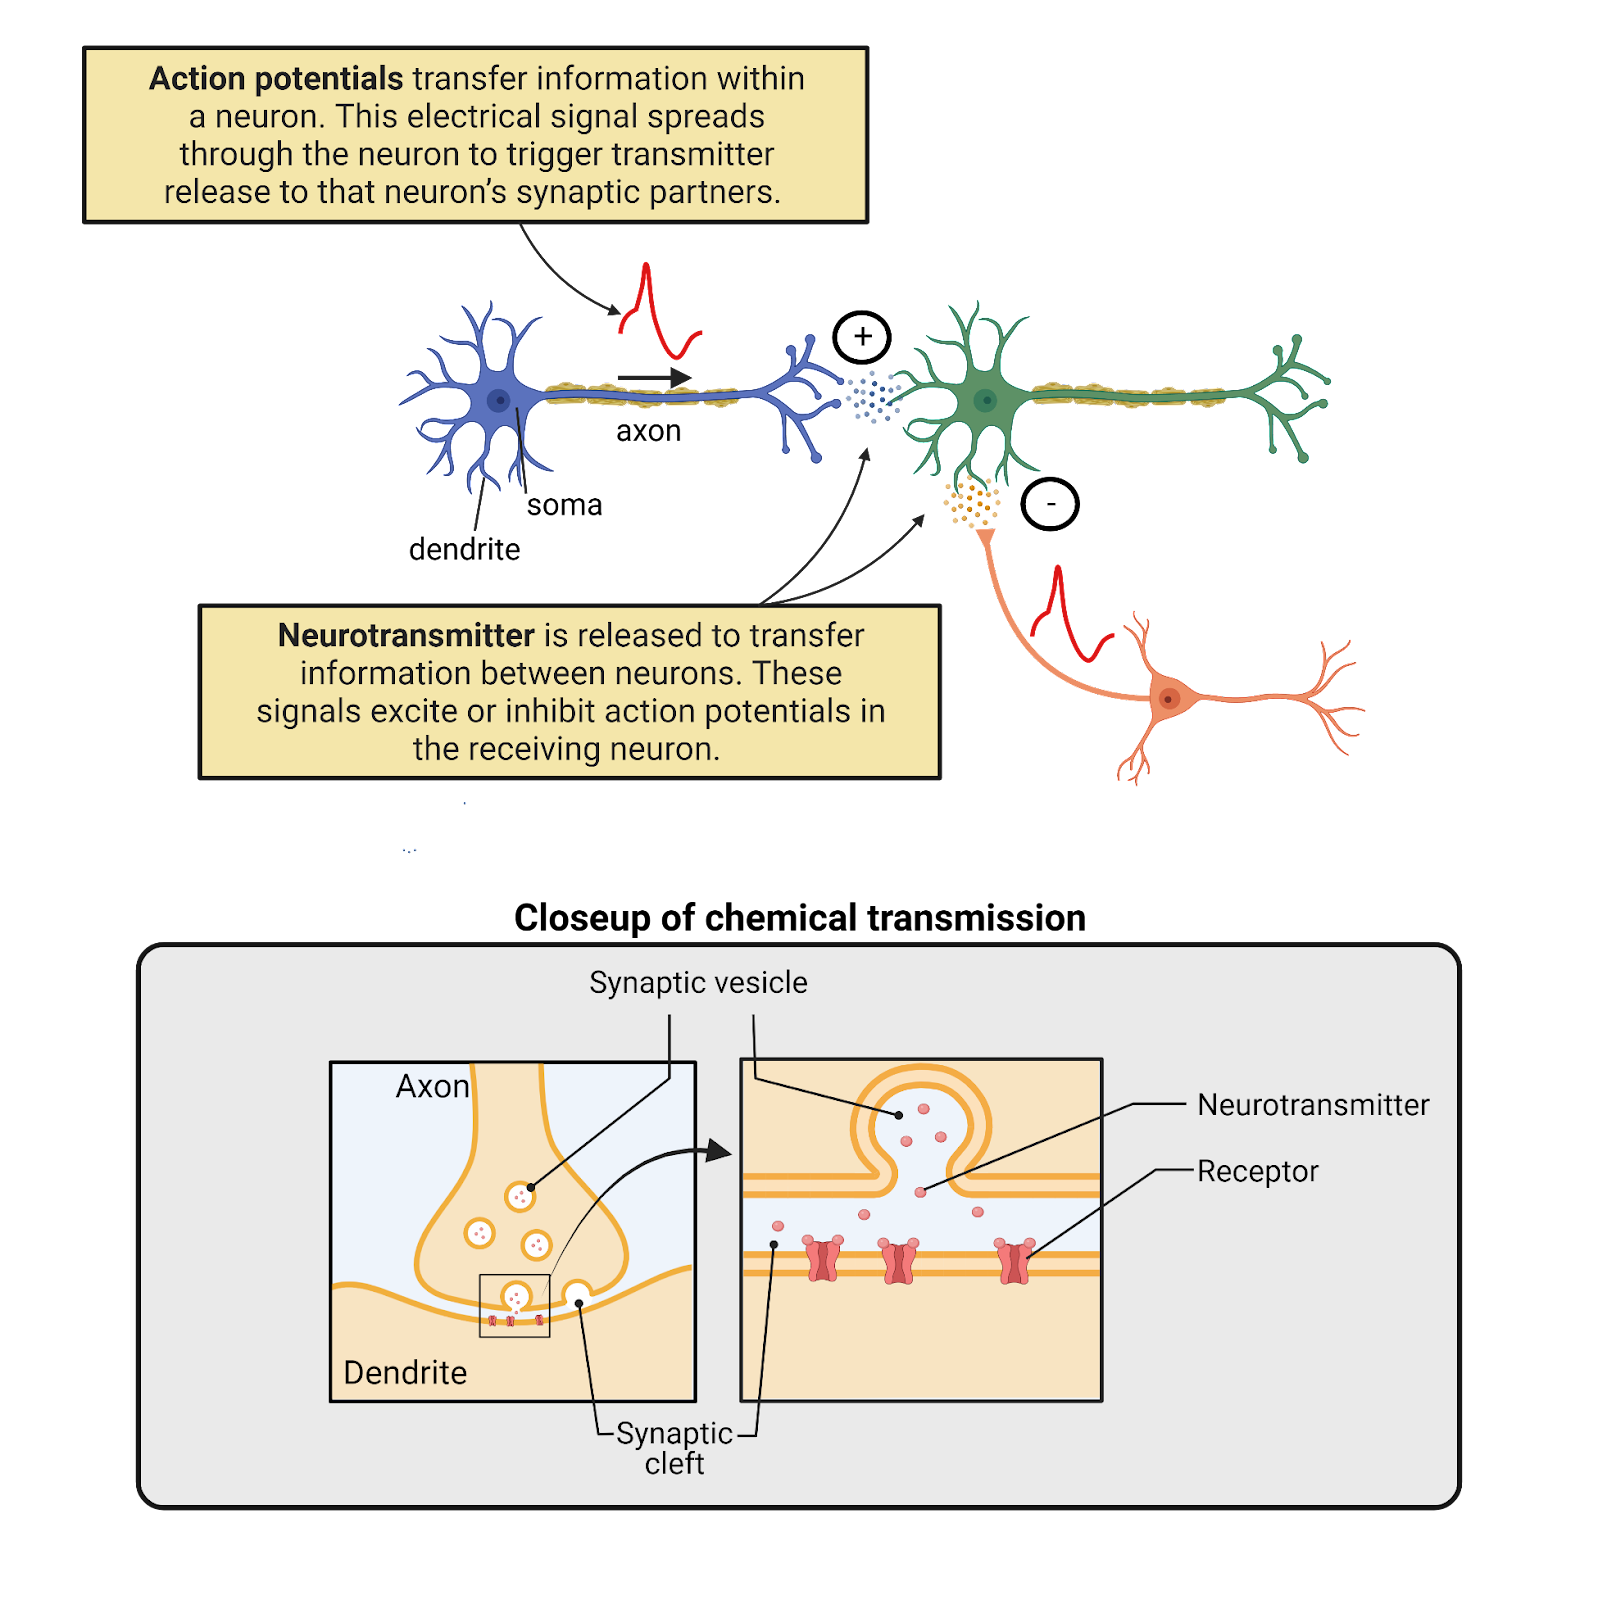
\includegraphics[width=0.8\linewidth]{images/ch02/02_01} 

}

\caption{Neurons are bilingual.}(\#fig:ch02_01)
\end{figure}

\hypertarget{communication-between-neurons-happens-chemically-at-synapses}{%
\subsection{\texorpdfstring{Communication between neurons happens chemically, at \textbf{synapses}}{Communication between neurons happens chemically, at synapses}}\label{communication-between-neurons-happens-chemically-at-synapses}}

\begin{figure}

{\centering 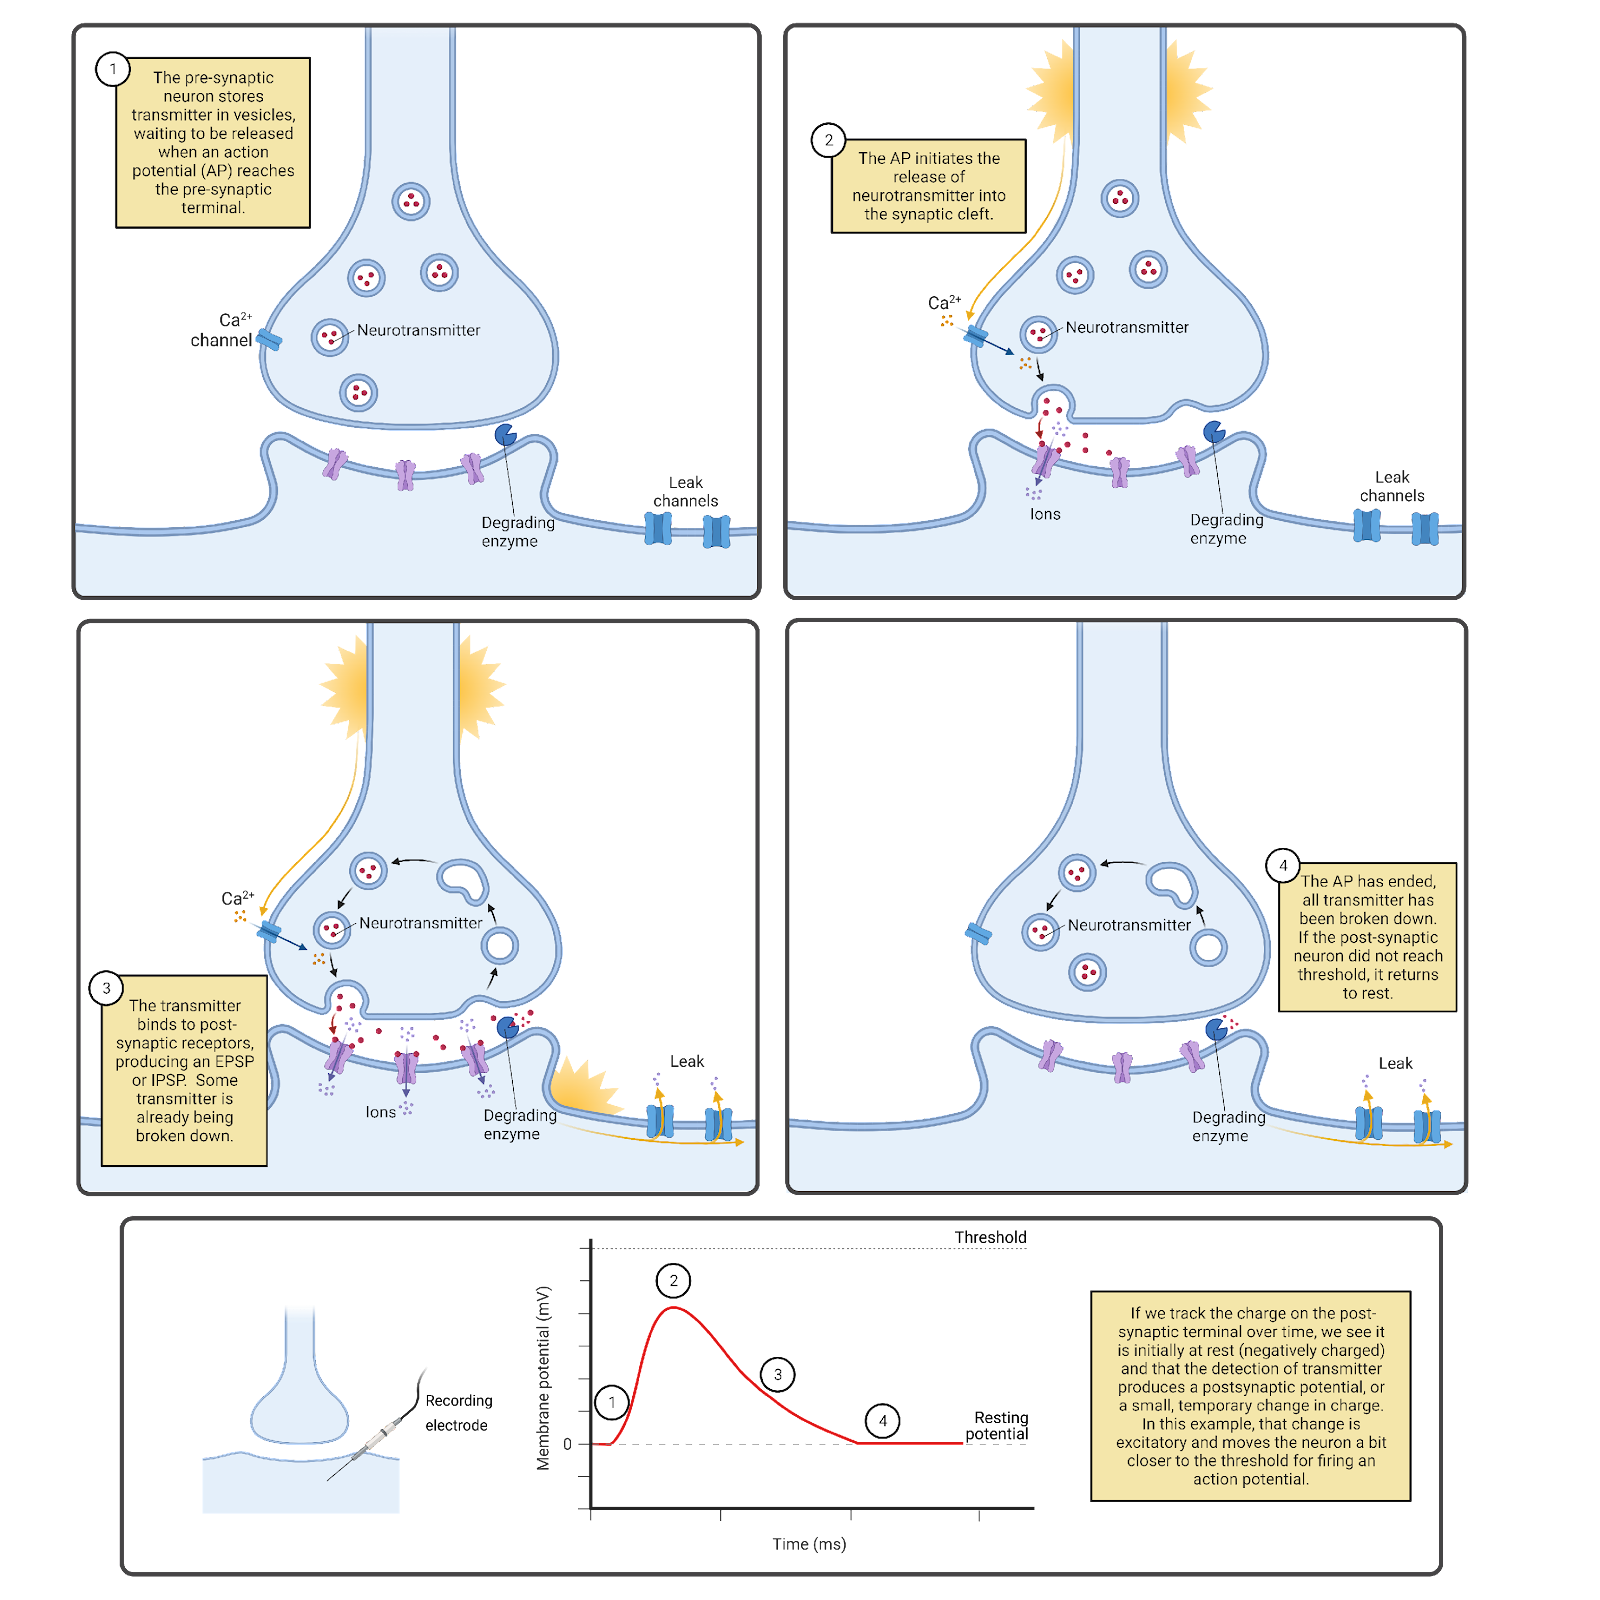
\includegraphics[width=0.8\linewidth]{images/ch02/02_02} 

}

\caption{Communication between neurons occurs primarily at **chemical synapses**.}(\#fig:ch02_02)
\end{figure}

The chemical signaling that occurs between neurons happens primarily at \textbf{chemical synapses} (Image 2:02), specialized communication structures where a broadcasting neuron and a receiving neuron draw very close to one another, separated only by a small pocket of intracellular space called a \textbf{synaptic cleft}. One neuron releases transmitter into the synaptic cleft---we call this the \textbf{pre-synaptic neuron}. The other neuron is studded with specialized receptors that recognize the transmitter and respond to it---we call this the \textbf{post-synaptic} neuron. There are many different neurotransmitters and many different transmitter receptors. Despite this complexity, each chemical message received is translated by receptors into one of just three responses in the post-synaptic neuron:

\begin{itemize}
\item
  An \textbf{Excitatory Post-Synaptic Potential} (\textbf{EPSP}), a brief electrical change in the post-synaptic neuron that \emph{excites} the neuron, pushing it towards firing an action potential.
\item
  An \textbf{Inhibitory Post-Synaptic Potential Inhibition} (\textbf{IPSP}), a brief electrical change in the post-synaptic neuron that \emph{inhibits} the neuron, pushing it away from firing an action potential.
\item
  \textbf{Neuromodulation}, a change in intracellular signaling in the post-synaptic neuron that \emph{modulates} that neuron, changing its patterns of growth, connectivity, or signaling.
\end{itemize}

Almost as soon as it is released, neurotransmitter is broken down and recycled, inactivating the receptors on the post-synaptic membrane. This ensures your synapses don't clog up with accumulated neurotransmitter over time. More importantly, it tunes neural communication to the here and now, making their messages to one another extremely \emph{transient} (short-lived). Each EPSP and IPSP lasts only a few milliseconds. The one exception to this rule is modulation, which is usually short-lived, but which can also become long-lasting; more details on modulation are in the chapter on Neurochemistry.

The chemical communication that occurs between neurons is a specialization of systems that appeared very early in the history of life. Even bacteria can secrete chemicals and have receptors that stick through their membranes to detect and respond to chemicals in their environment. Many of the neurotransmitters and transmitter receptors used in your nervous system have long evolutionary histories, so it is not uncommon to find similar chemicals and proteins both in other forms of life and in other parts of your body. For example, histamine is an important neurotransmitter, but is also produced in white blood cells as part of an immune response to injury. This is part of the reason why substances in the natural world can influence your nervous system (caffeine!) and why drugs developed to treat brain disorders often have unwanted side effects in other parts of the body.

Although chemical communication between neurons has ancient roots, it has become highly specialized in neurons. One key specialization is that chemical communication is precisely \emph{targeted}. Neurons release neurotransmitter almost exclusively at synapses. The tiny volume of the synaptic cleft ensures the post-synaptic neuron \emph{will} get the message, and that other neurons (for the most part) will not. The pre-synaptic membrane also has specialized protein machinery to maintain a steady supply of neurotransmitter for release, and the post-synaptic side is loaded with receptors as well as other proteins that anchor the receptors and help fine-tune the responses to synaptic signals.

Although \emph{most} communication between neurons occurs via chemical synapses, neurons can also signal to each other through what are called \textbf{electrical synapses }(Image 2.03). At an electrical synapse, neurons express a specialized protein, called \textbf{connexon}, which forms a protein bridge between the neurons. This enables electrical signals to pass directly from one neuron to another. In addition, small molecules can pass through an electrical synapse, so they actually allow for both electrical and chemical communication.

If you find communication between neurons fascinating, you're not alone and you're also in luck. When you get to the chapter on Neurochemistry, you'll read more about chemical communication between neurons.

\begin{figure}

{\centering 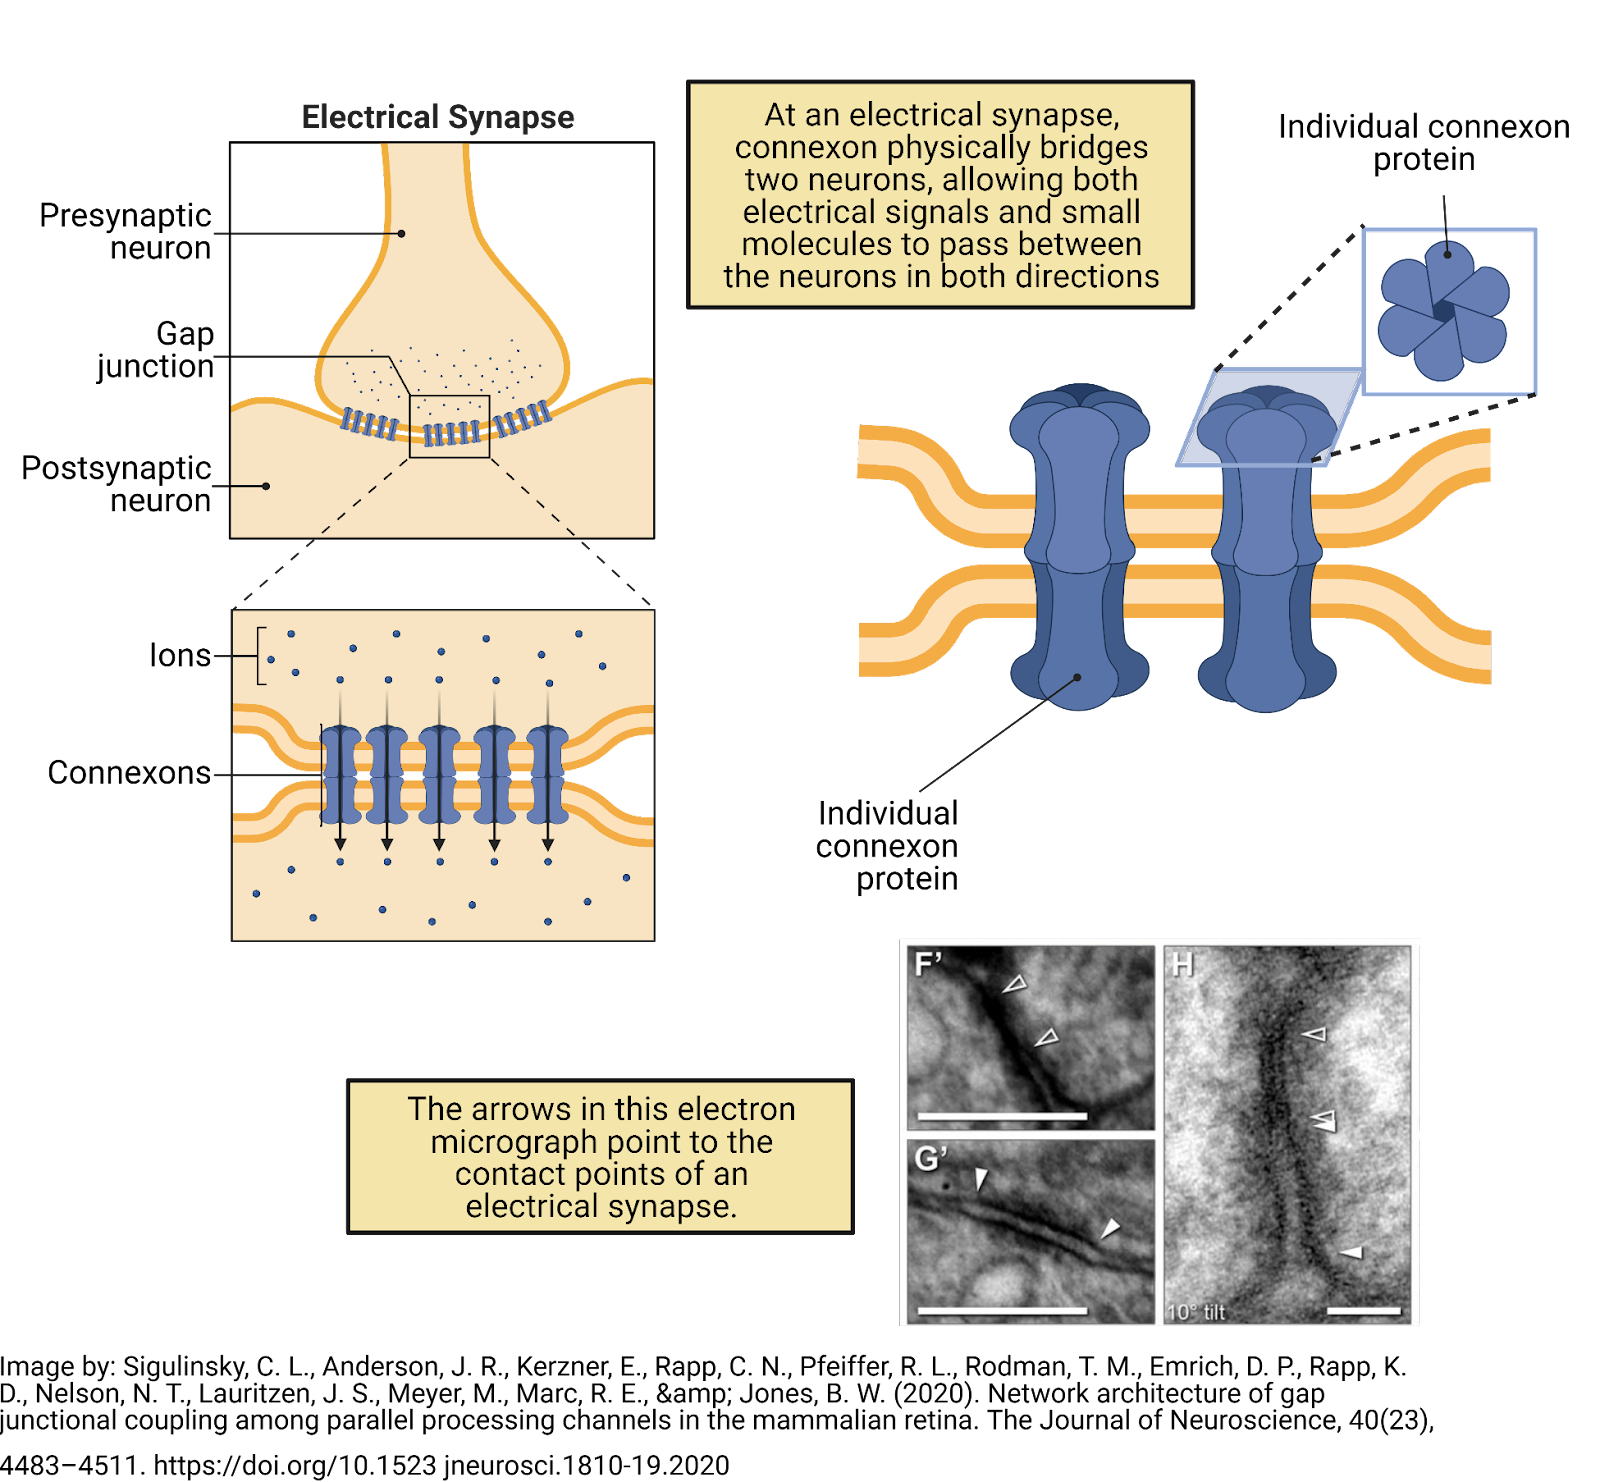
\includegraphics[width=0.8\linewidth]{images/ch02/02_03} 

}

\caption{Communication between neurons also occurs at **electrical synapses**.}(\#fig:ch02_03)
\end{figure}

\hypertarget{information-spreads-within-a-neuron-electrically}{%
\subsection{Information spreads within a neuron electrically}\label{information-spreads-within-a-neuron-electrically}}

Neurons are specialized not only for communicating with each other, but also for generating internal electrical signals (Image 2:04). Like almost all cells, neurons maintain an overall negative charge called a \textbf{resting potential}. In addition, neurons are \emph{electrically excitable}; generating \textbf{action potentials} that sweep through a neuron at speeds up to 60 meters per second (134 miles per hour; Todnem et al., 1989). Each action potential is translated back into chemical messages released to partner neurons.

\begin{figure}

{\centering 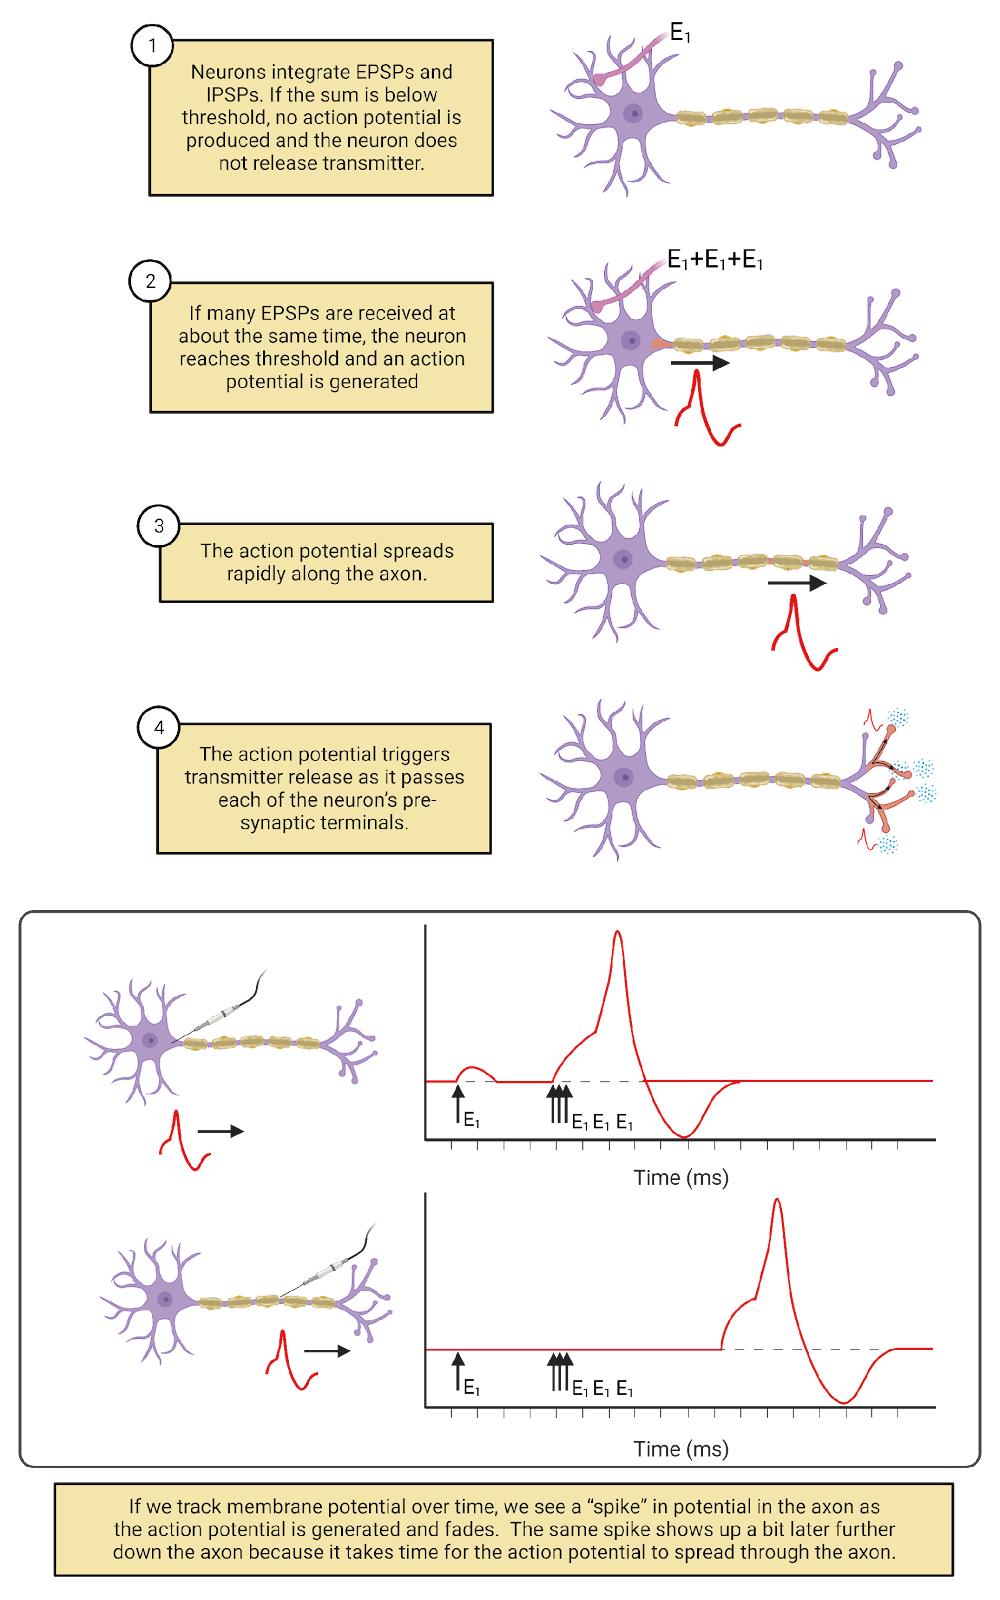
\includegraphics[width=0.8\linewidth]{images/ch02/02_04} 

}

\caption{Action potential spread and neurotransmitter release.}(\#fig:ch02_04)
\end{figure}

How does a neuron decide when to ``fire'' an action potential? Based, in part, on the constant barrage of chemical messages it is receiving on the post-synaptic side of its synaptic contacts. The EPSPs and IPSPs produced by these messages push a neuron above or below its \textbf{threshold} for generating an action potential. When the balance of excitation and inhibition being received is below a neuron's threshold, the neuron does not fire an action potential or release transmitter to its partner neurons. When the balance of excitation and inhibition rises above a neuron's threshold, it fires an action potential. The action potential spreads from the cell body along the length of the axon and all of its branches. As it spreads, the action potential is translated back into chemical messages, triggering the release of neurotransmitter from the pre-synaptic side of all the neuron's synaptic contacts. A neuron firing an action potential is said to be \emph{activated} or \emph{excited}, with each action potential producing a burst of chemical signals to its synaptic partners.

The more excitation a neuron receives, the more \emph{frequently} it fires action potentials. But this doesn't make the action potential itself taller, stronger, or faster. Action potentials are `all-or-nothing'---each action potential a neuron generates is basically just like another. There can be, however, considerable diversity \emph{between} neurons. For example, some neurons fire action potentials that spread very quickly; others fire action potentials that spread more slowly. In addition, neurons are highly dynamic. Experience, disease, and maturation can change a neuron's threshold, which synaptic partnerships it maintains, and more. For example, modulatory signaling in your nervous system is constantly fine-tuning action potential thresholds, lowering them to produce more activity during times of concentration and raising them to produce less activity during rest and sleep (more on this in the chapter on Circadian Rhythms and Sleep).

Excitation and inhibition from partner neurons are not the only factors that determine when a neuron fires an action potential (Image 2.05). Some neurons fire action potentials in response to changes in the outside world. We call these \textbf{sensory neurons}. In addition, most neurons in your nervous system generate action potentials \emph{spontaneously}, meaning that they generate action potentials from time to time even without excitatory messages from partner neurons. For example, \textbf{motor neurons}, the neurons which release transmitter onto muscles, are often spontaneously active. This regular activity in your motor neurons maintains muscle tone (Motor Control{]}). In spontaneously active neurons, EPSPs and IPSPs from partner neurons serve to speed up (when excited) or slow down (when inhibited) the rate at which action potentials are fired.

\begin{figure}

{\centering 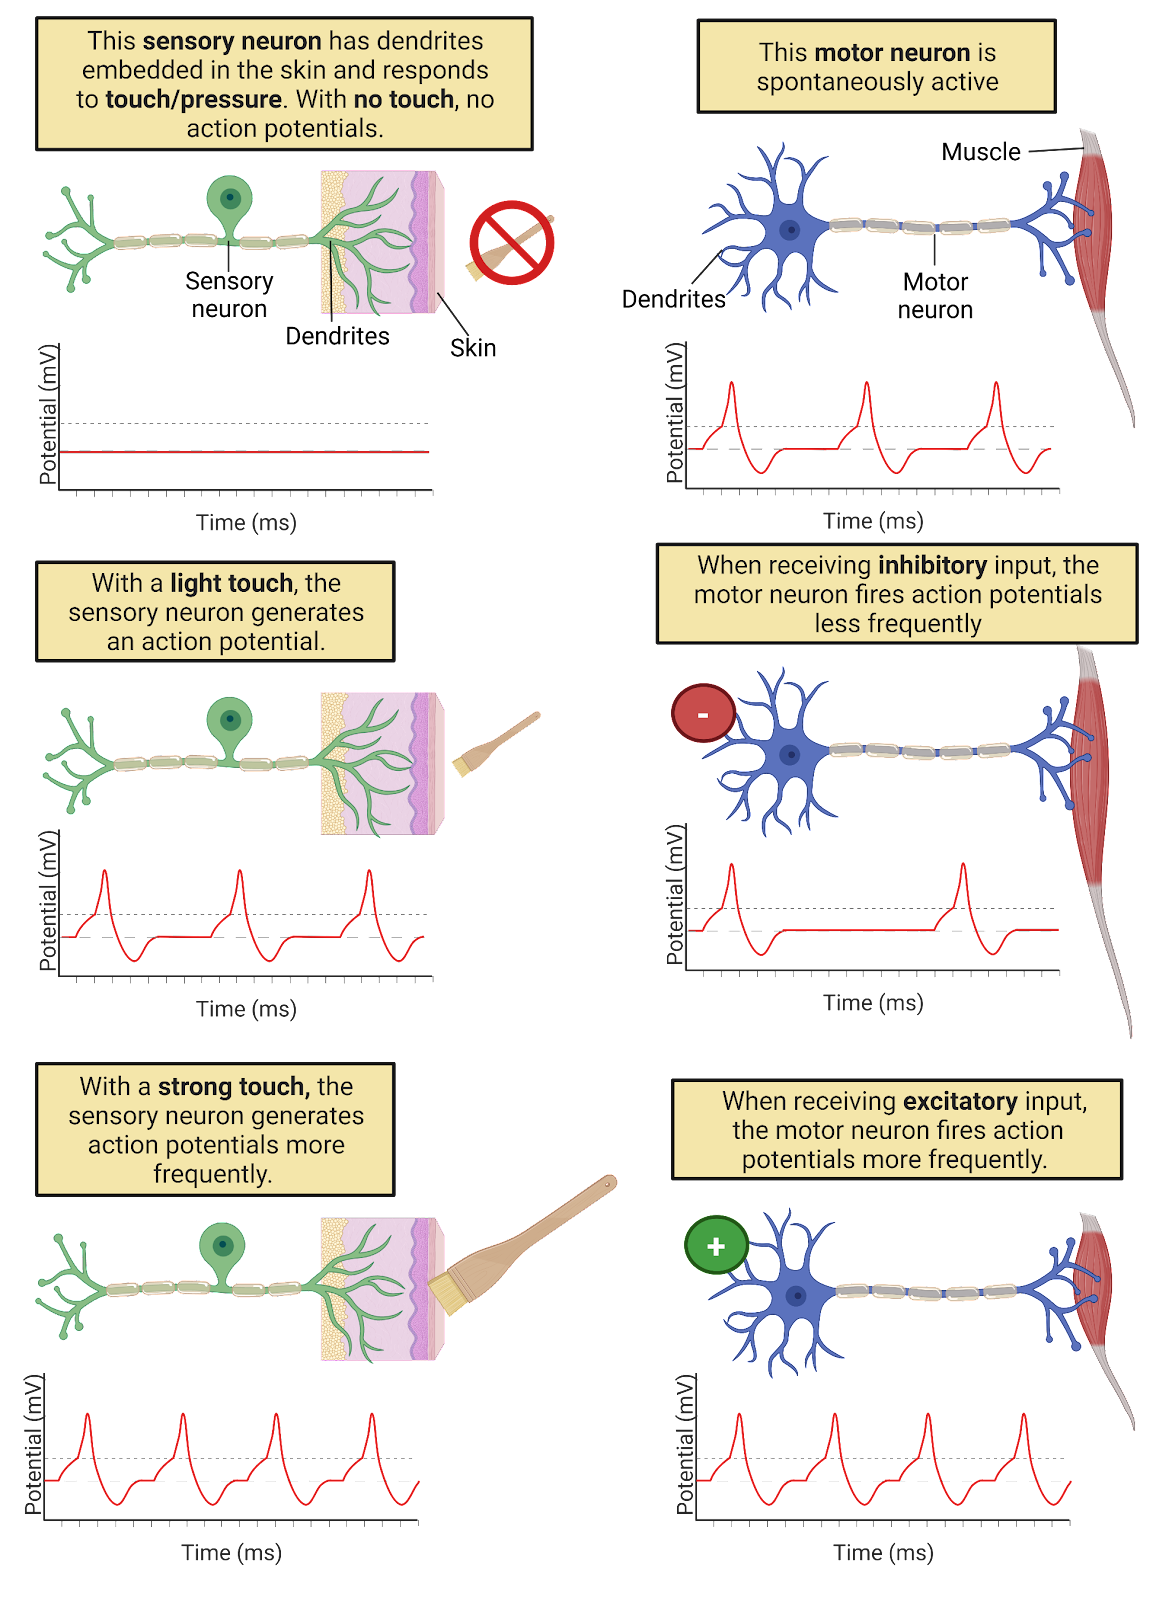
\includegraphics[width=0.8\linewidth]{images/ch02/02_05} 

}

\caption{There are internal and external triggers for action potentials.}(\#fig:ch02_05)
\end{figure}

The electrical signaling system in neurons is relatively new in the history of life, emerging at the dawn of the Animal kingdom at least 500 million years ago (though with important precursors in other life forms; Anctil, 2015). Electrical signaling enables neurons to coordinate information throughout your body with speed and precision, something that would be difficult to do with chemical communication alone. For example, you have sensory neurons in your toe (Image 2:06). The axons of these neurons ascend in your sciatic nerve to the base of your spine (depending on how tall you are, that can be a distance of up to 1 meter!). Pinch your big toe and you will trigger action potentials in your toe sensory neurons that spread to the spine within a couple of milliseconds, releasing transmitter onto partner neurons. Some of these partner neurons will send signals back down to the muscles of your leg and foot to cause muscle contractions to jerk your foot away from the pain. Other neurons will generate action potentials that spread rapidly to the brain, hopefully triggering you to question your life choices: \emph{Why would you pinch your big toe? Just because your neuroscience textbook told you to?}

\begin{figure}

{\centering 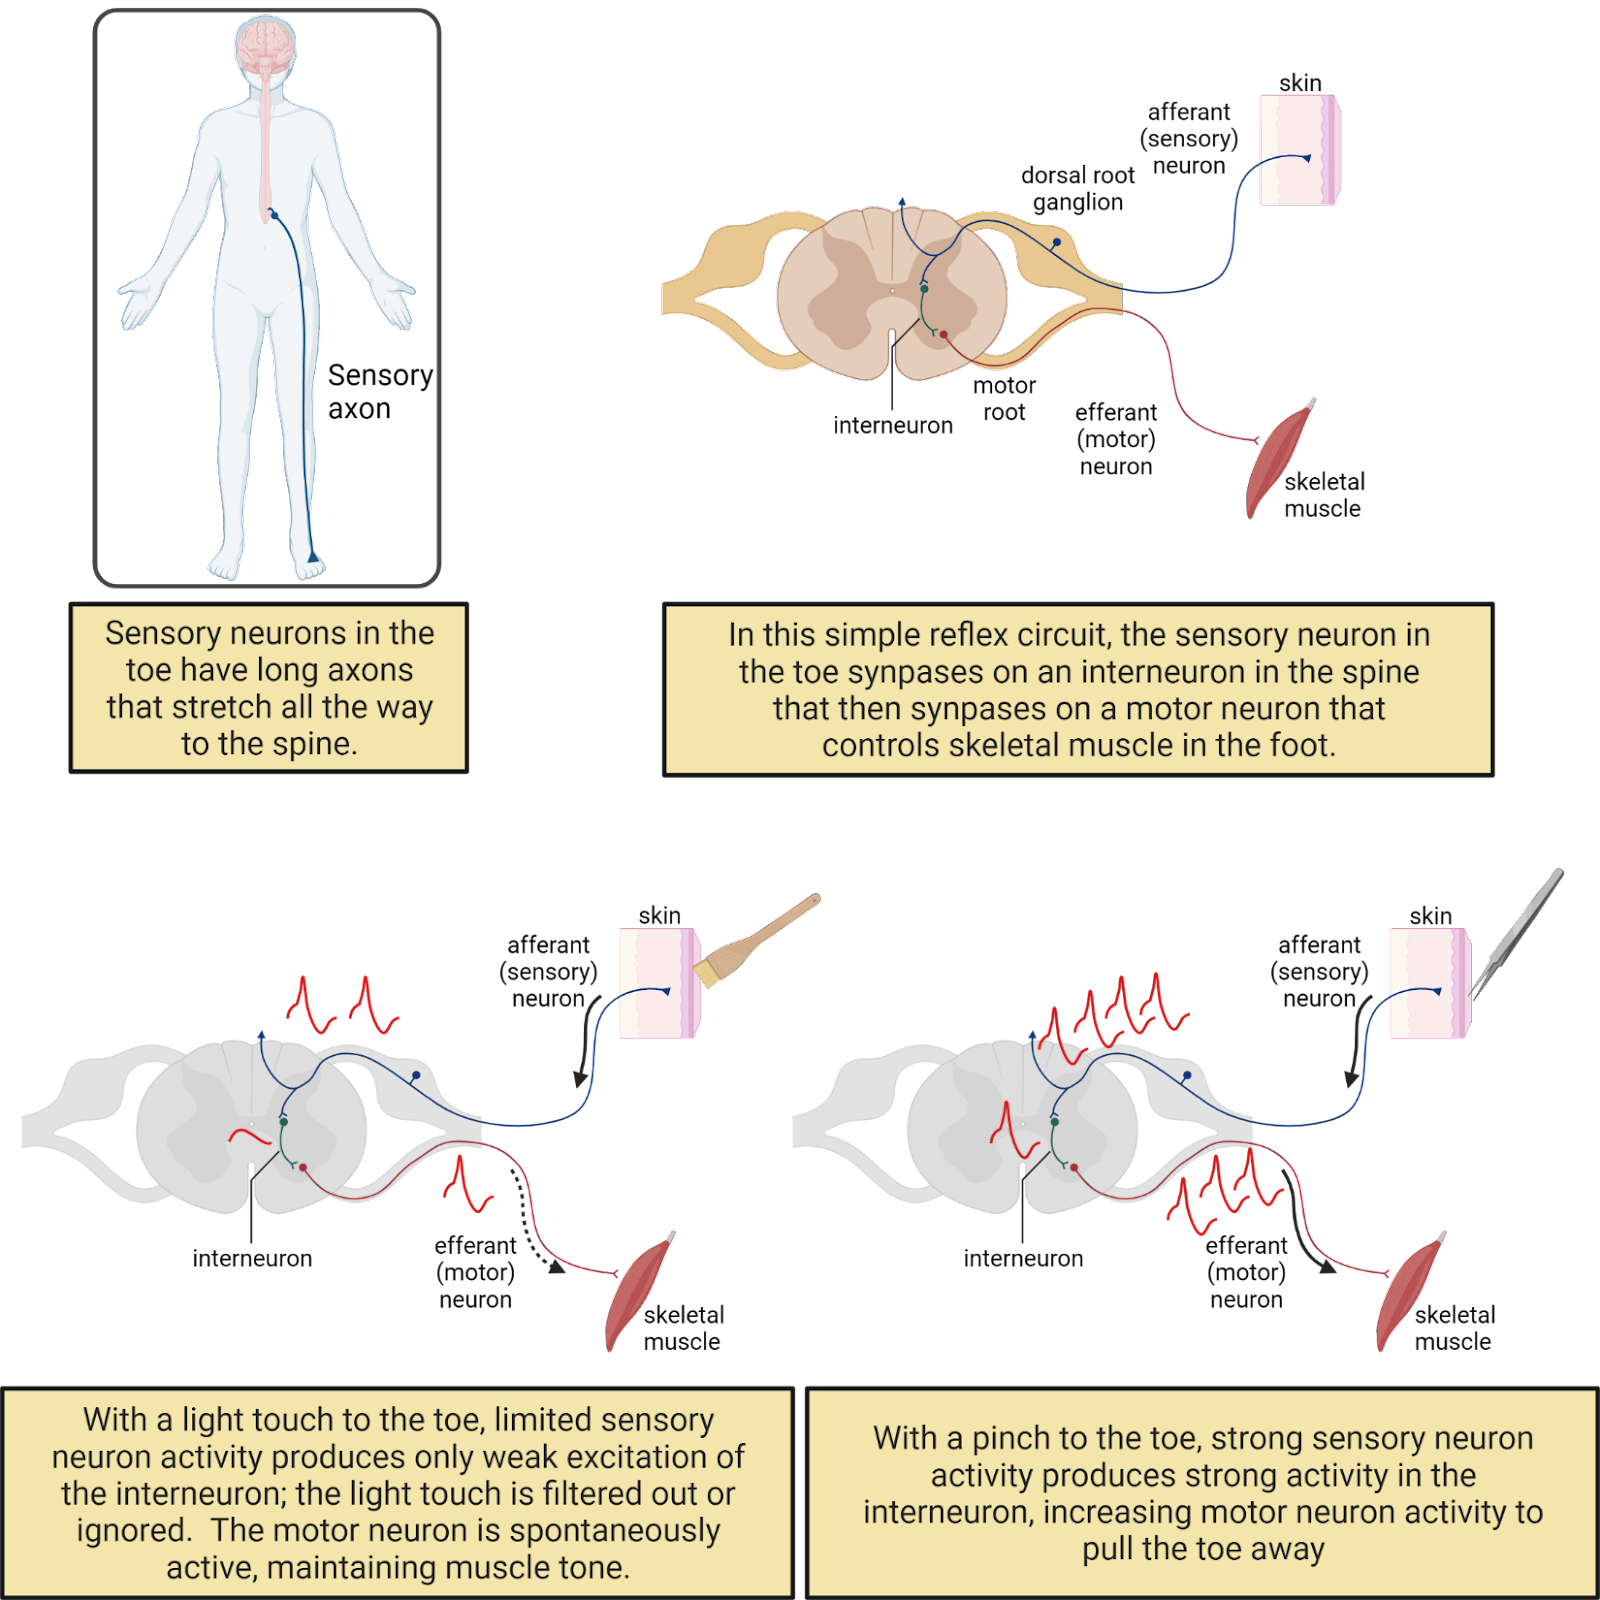
\includegraphics[width=0.8\linewidth]{images/ch02/02_06} 

}

\caption{Neurons form circuits.}(\#fig:ch02_06)
\end{figure}

Neurons don't just transfer information; they also \emph{process} information. Each neuron \emph{synthesizes} the excitation and inhibition received from thousands of synaptic partners, instantly tallying up these different influences to help determine when an action potential will be generated. In addition, the threshold for an action potential means that neurons \emph{filter} information. Inputs that push a neuron above threshold produce action potentials, which then cause neurotransmitter release to partner neurons. Inputs that do not reach threshold are essentially `ignored' or filtered out.

\hypertarget{topic-summary}{%
\subsection{Topic summary}\label{topic-summary}}

Neurons are bilingual, using two inter-related but distinct signaling systems. Communication \emph{between} neurons primarily uses the ancient language of chemical and receptor that all your cells use, though with adaptations for highly targeted and reliable communication. Grafted onto this ancient system is an electrical signaling system that transfers information \emph{within} a neuron with a level of speed and precision that is relatively unique to the animal kingdom. An engineer probably wouldn't have designed such a complex system. Instead, the hybrid nature of neural signaling reflects the piecemeal adaptation of nervous system functioning through a long evolutionary history. From this complexity emerges neural processing. The back-and-forth-and back-again transformation from chemical to electrical to chemical signaling enables neurons to synthesize, filter, and transform information in complex and fascinating ways.

\textbf{Key Terms}

\begin{itemize}
\item
  Neurotransmitters
\item
  Action potentials
\item
  Chemical synapses
\item
  Synaptic cleft
\item
  Pre-synaptic
\item
  Post-synaptic
\item
  Excitatory Post-Synaptic Potential (EPSP)
\item
  Inhibitory Post-Synaptic Potential (IPSP)
\item
  Electrical Synapse
\item
  Connexion
\item
  Resting Potential
\item
  Threshold
\item
  Sensory Neuron
\item
  Motor Neuron
\end{itemize}

\textbf{References and works cited}

\begin{itemize}
\item
  Anctil M (2015) Dawn of the Neuron: The Early Struggles to Trace the Origin of Nervous Systems. Montreal \& Kingston, London, Chicago: McGill-Queen's University Press.
\item
  Herculano-Houzel S (2012) The remarkable, yet not extraordinary, human brain as a scaled-up primate brain and its associated cost. Proc Natl Acad Sci U S A 109:10661--10668.
\item
  Pakkenberg B, Pelvig D, Marner L, Bundgaard MJ, Gundersen HJG, Nyengaard JR, Regeur L (2003) Aging and the human neocortex. Exp Gerontol 38:95--99.
\item
  Testa-Silva G, Verhoog MB, Linaro D, de Kock CPJ, Baayen JC, Meredith RM, De Zeeuw CI, Giugliano M, Mansvelder HD (2014) High Bandwidth Synaptic Communication and Frequency Tracking in Human Neocortex. PLoS Biol 12.
\item
  Todnem K, Knudsen G, Riise T, Nyland H, Aarli JA (1989) The non-linear relationship between nerve conduction velocity and skin temperature. J Neurol Neurosurg Psychiatry 52:497--501.
\end{itemize}

\hypertarget{neurophysiology-circuits}{%
\section{Neural circuits}\label{neurophysiology-circuits}}

\textbf{Learning objectives}

By the end of this section, students will be able to:

\begin{itemize}
\item
  Objective 1: Describe the rhythmic behavior produced by the simple swim circuit in \emph{Tritonia diomedia}
\item
  Objective 2: Define some of the key features of neural circuits: parallel processing, feedback, efficiency, and a careful balance between excitation and inhibition
\item
  Objective 3: Describe the work of computational neuroscientists to build mathematical models of neurons and neural circuits
\end{itemize}

As specialists in communication, neurons do not work on their own, but in interconnected groups, often called a \textbf{neural circuit} or a \textbf{neural network}. Even small numbers of neurons can generate remarkably complex behavior. To see this, let's examine a very simple neural circuit: the ``swim'' network in the sea slug \emph{Tritonia Diomedea}.

\hypertarget{in-the-swim-circuit-of-tritonia-diomedia-a-few-neurons-produce-rhythmic-behavior-important-for-survival.}{%
\subsection{\texorpdfstring{In the ``swim'' circuit of \emph{Tritonia diomedia} a few neurons produce rhythmic behavior important for survival.}{In the ``swim'' circuit of Tritonia diomedia a few neurons produce rhythmic behavior important for survival.}}\label{in-the-swim-circuit-of-tritonia-diomedia-a-few-neurons-produce-rhythmic-behavior-important-for-survival.}}

\emph{Tritonia} is a species of slimy mollusk that glides along the ocean floor off the west coast of the United States and Canada (Image 2:07). The mortal enemy of a \emph{Tritonia} is the Pacific sea star, a voracious predator that loves to dine on \emph{Tritonia} if it can. To avoid this fate, a \emph{Tritonia} ``swims'' away if it feels the touch of a sea star. Well, actually the \emph{Tritonia} kind of thrashes about, arching its back, then relaxing, then arching again, in a rhythmic motion that helps it move up into the ocean current. When the \emph{Tritonia} stops swimming, it sinks back down to the ocean floor, hopefully far away from the hungry sea star. Check out a video of a \emph{Tritonia} escaping a sea star here:\url{https://www.youtube.com/watch?v=JCr1b1mJWoU}.

\begin{figure}

{\centering 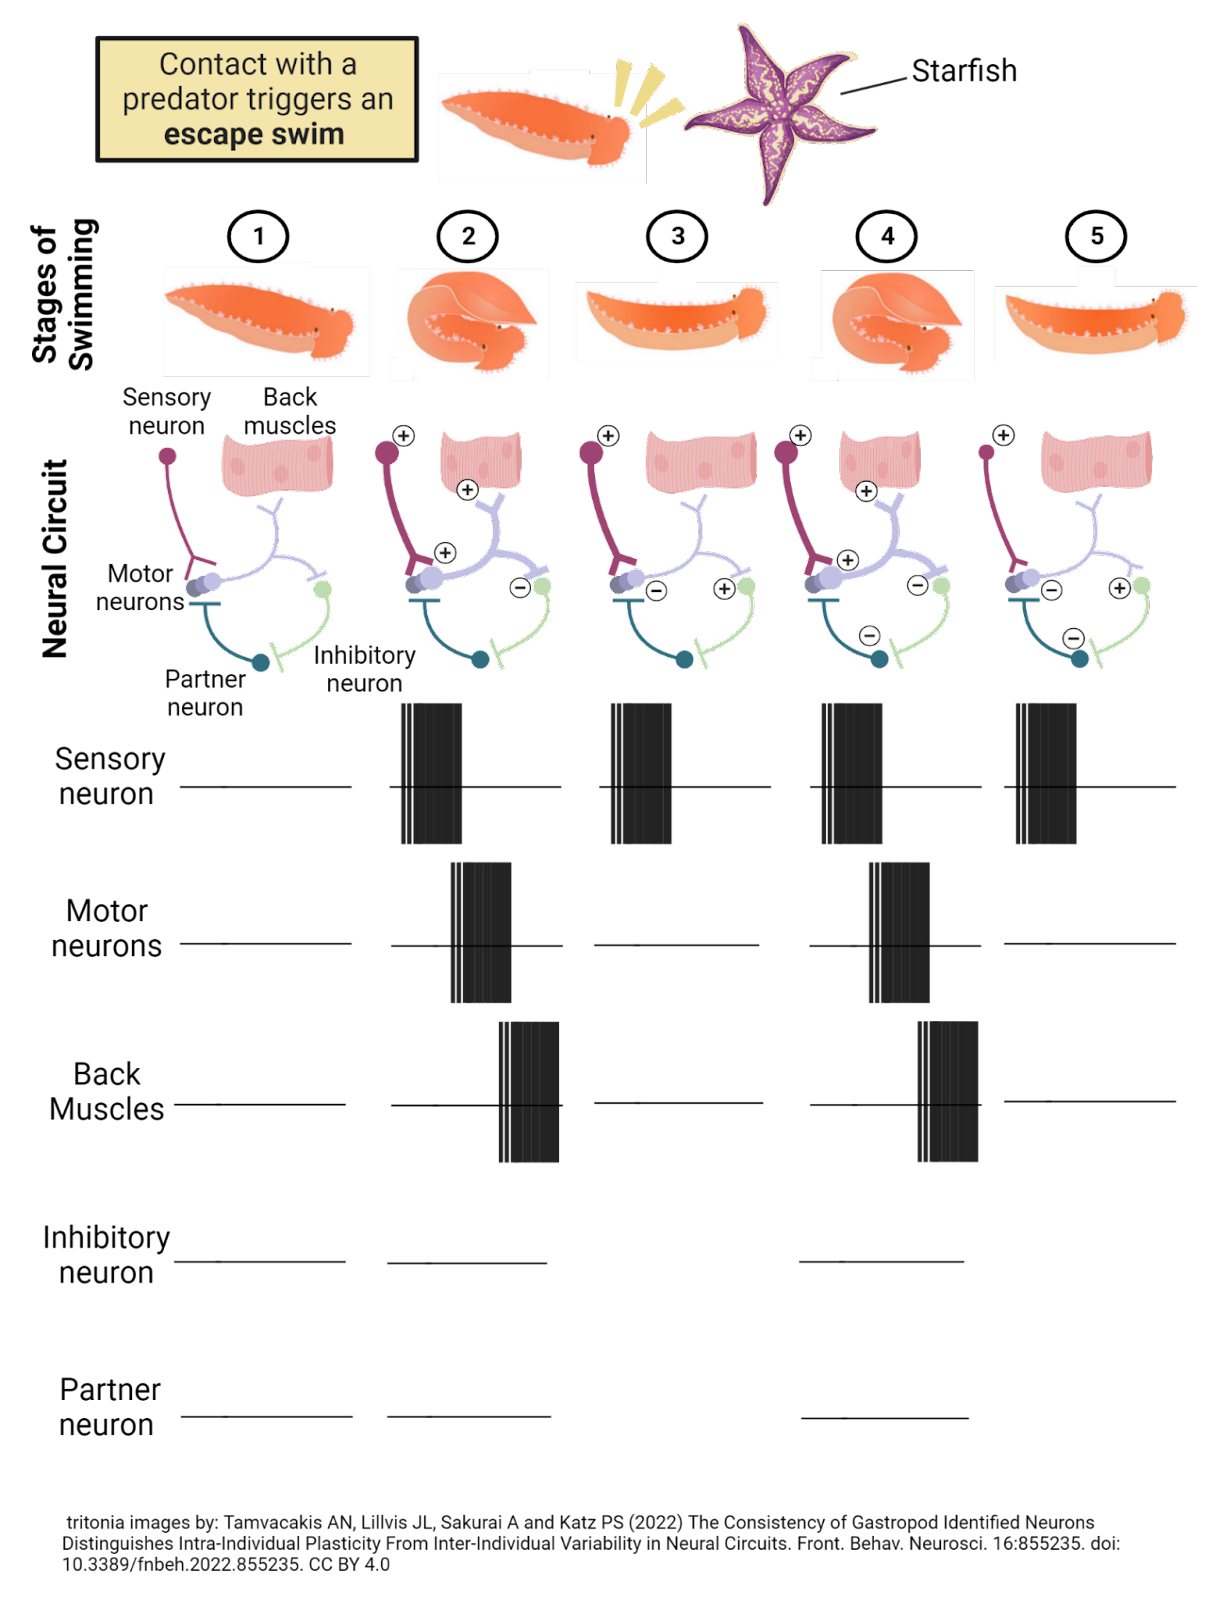
\includegraphics[width=0.8\linewidth]{images/ch02/02_07} 

}

\caption{The “swim” circuit in Tritonia Diomedea.}(\#fig:ch02_07)
\end{figure}

Researchers have found that \emph{Tritonia} swim away from danger with the help of a relatively simple neural circuit (Willows and Hoyle, 1969; Getting, 1983). Sensory neurons in the skin are tuned to specific chemicals on the tentacles of the Pacific sea star. When these are detected, the sensory neurons become very excited, firing a long-lasting barrage of action potentials. The sensory neurons release excitatory transmitter onto a set of 3 motor neurons which control the muscles of the back. When these motor neurons reach threshold they fire action potentials, contracting the back muscles to produce the arching movement that forms the first half of the `swim' \textbf{rhythm }(a behavior that is cyclical or periodic).

This is not all the motor neurons do. They also release excitatory transmitter onto partner neurons, which in turn excite an \emph{inhibitory} neuron. This inhibitory neuron provides \textbf{feedback} to the circuit, inhibiting the motor neurons. When this happens, the inhibition overwhelms the excitatory input from the sensory neurons, and the motor neurons are pushed below threshold. With the motor neurons inactive, the back muscles relax and the \emph{Tritonia} straightens out. At this point, it has arched back and then relaxed forward, completing a `swim' rhythm.

You can probably work out the next, very interesting step in this circuit's function: with the motor neurons inactive, the inhibitory neuron is no longer being excited, so it stops firing action potentials and releases the motor neurons from inhibition. That means the long-lasting activity in the sensory neurons is again able to activate the motor neurons, producing another arching of the back, but then another round of inhibition leading to another relaxing forward. The whole cycle repeats over and over again until the sensory neurons stop firing, which usually takes 10 to 30 seconds. Thus, just a few neurons in the \emph{Tritonia} nervous system transform an outside event (a sea star touch) into a complex and long-lasting rhythm that `swims' it away from danger.

The \emph{Tritonia} swim network is not only rhythmic; it is also \emph{dynamic}, changing based on the \emph{Tritonia's} experience. For example, if a \emph{Tritonia} is injured, the sensory neurons become hyper-excitable, firing at a lower threshold and for longer times. This shifts the \emph{Tritonia} to be more likely to swim and to swim more vigorously, hopefully protecting it from further injury (but also using precious energy). The swim network can also shift in the other direction. If a \emph{Tritonia} is gently touched over and over again, the sensory neurons produce smaller and smaller EPSPs, and the network begins to ignore this gentle touch, learning that it does not pose a real danger (Brown, 1998; Hoppe, 1998). The dynamic nature of the swim network helps the Tritonia strategically allocate its energy based on its experiences---to swim away from real danger to while also saving energy by ignoring events that are \emph{innocuous} (meaning harmless or non-threatening).

The \emph{Tritonia} swim circuit is in some ways quite simple, involving the operation just 5 neurons in the CNS (not counting the sensory neurons that detect the sea-star touch). Still, things can go wrong. If the connection to the inhibitory neuron is weakened, there will not be enough inhibition to pause activity in the circuit, and instead the circuit will produce constant activity that could lock up the back muscles, freezing the \emph{Tritonia} in an arched position that will make it into an easy dinner. Too much inhibition is also problematic. If the inhibitory neuron releases too much neurotransmitter, the circuit would pause for too long, letting the animal drop back down to the ocean floor before it has managed to get away from the sea star. Generating the swim rhythm that keeps a \emph{Tritonia} safe requires just the right balance between excitation and inhibition to keep the circuit moderately but not excessively activated (Katz and Frost, 1997; Calin-Jageman et al., 2007).

\hypertarget{studying-neural-circuits-reveals-important-principles-about-how-nervous-systems-generate-behavior.}{%
\subsection{Studying neural circuits reveals important principles about how nervous systems generate behavior.}\label{studying-neural-circuits-reveals-important-principles-about-how-nervous-systems-generate-behavior.}}

You probably never thought about the swimming behaviors of slimy mollusks before, but hopefully you found it exciting (pun intended) to learn how just a few neurons can produce a life-saving behavior. One of the key goals of neuroscience is to uncover the secrets of more complex neural networks, such as the ones operating in your nervous system to produce language, emotions, and thought. There is still a lot we do not know, but even from the simple swim circuit of \emph{Tritonia} we can glean a few key insights (Image 2.08):

\begin{figure}

{\centering 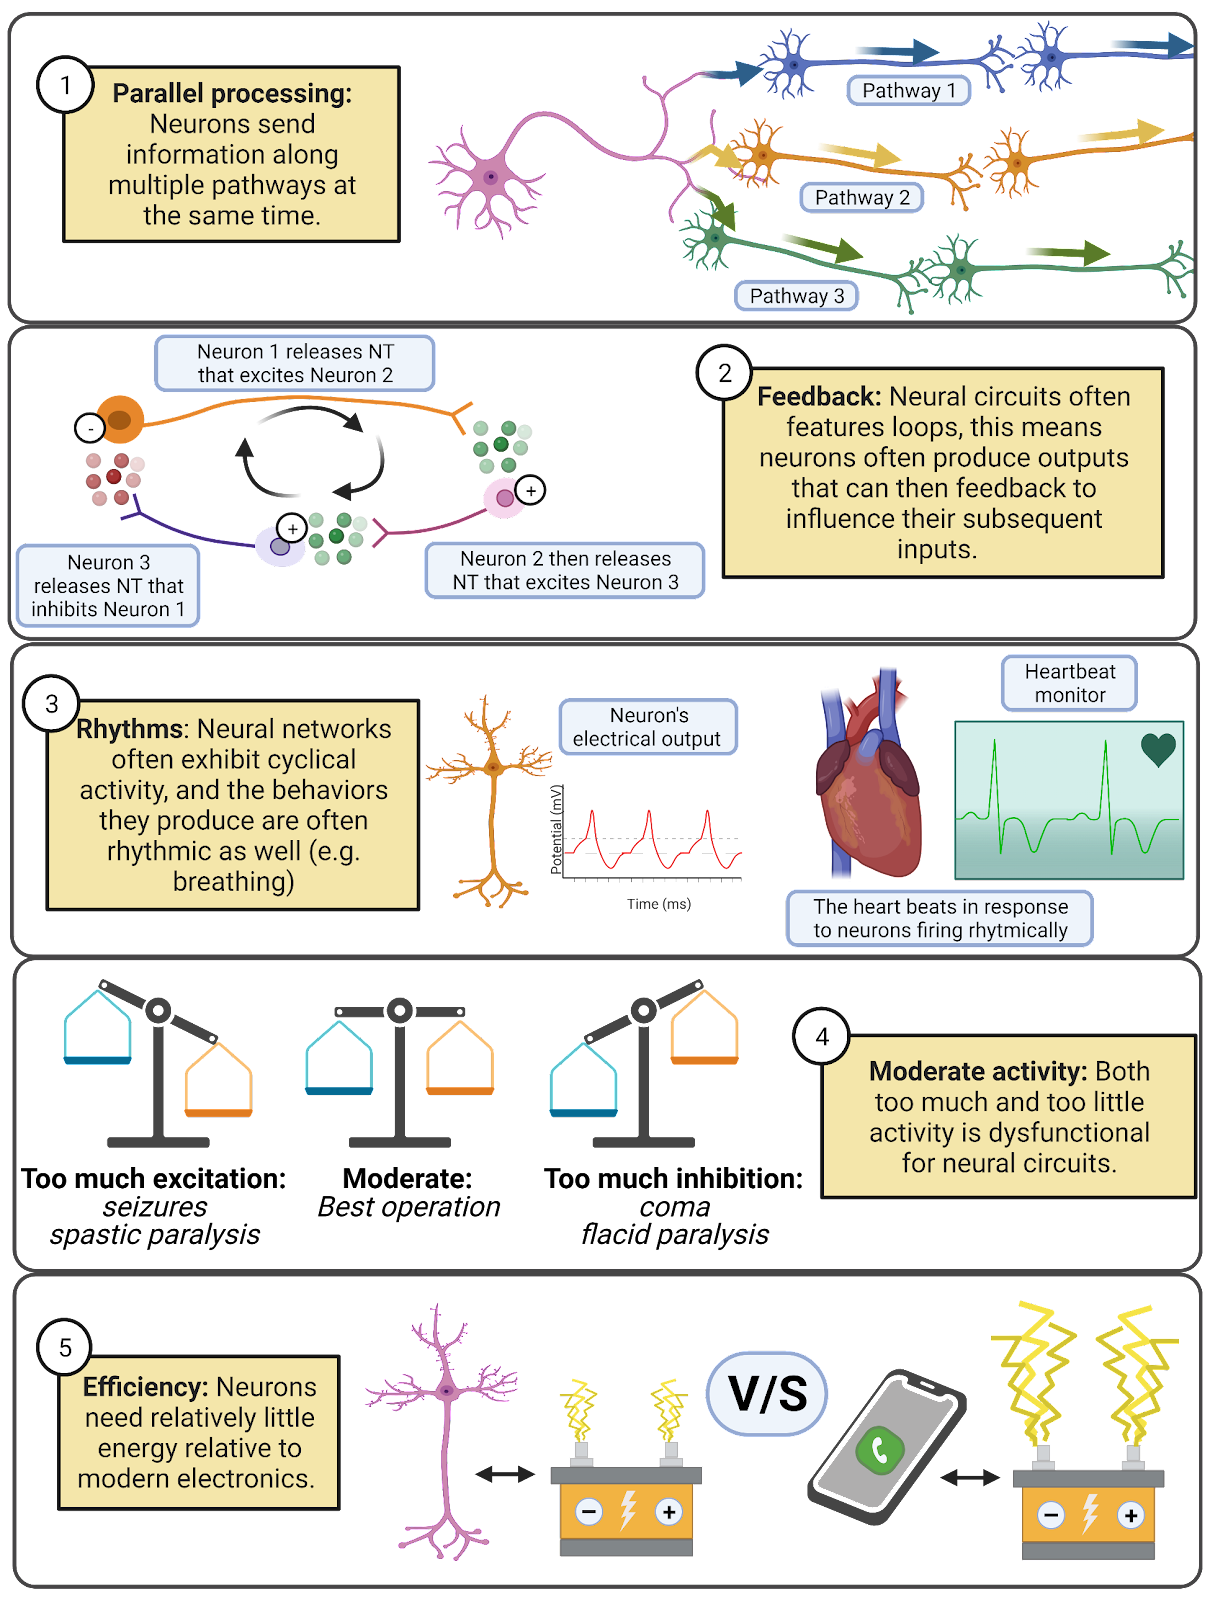
\includegraphics[width=0.8\linewidth]{images/ch02/02_08} 

}

\caption{Principles of neural circuits.}(\#fig:ch02_08)
\end{figure}

\begin{itemize}
\tightlist
\item
  Neural networks feature \textbf{parallel processing, }meaning that information spreads along multiple pathways. In the \emph{Tritonia} swim network, the motor neurons form synapses onto the muscles \emph{and} onto a partner neuron that activates inhibition, sending messages along two distinct pathways at the same time.
\item
  Feedback, where a neuron influences the inputs it will later receive, makes even seemingly simple networks capable of producing complex patterns of activity.
\item
  Neural networks are often rhythmic or cyclical, exhibiting repeating patterns of activity and inactivity. This is reflected in the fact that many of our behaviors are also rhythmic: walking, sleep/wake cycles, breathing, and more. The chapter on Circadian Rhythms and Sleep digs into detail on these fascinating cycles of neural activity.
\item
  Neural circuits can malfunction. They operate best at moderate levels of activity. They can easily be overwhelmed with excitation (which shows up in behavior as seizures or muscle \emph{spasticity}) or inhibition (which shows up in behavior as torpor or muscle \emph{flaccidity}). To work well, networks need both inhibition and excitation, and in the right balance.
\item
  Neural networks are highly efficient. \emph{Tritonia} can swim away from danger with a network of just 5 neurons. Even with the large numbers of neurons in the mammalian nervous system, the efficiency of operation is incredible. Your entire brain uses about 20 watts of electrical power (Balasubramanian, 2021). For comparison, a modern Xbox or Playstation draws up to 160 watts of power. It is true that your brain uses a large fraction of your daily energy budget (about 500 kilocalories per day, or 25\% of a typical 2,000 kilocalorie daily energy budget; Herculano-Houzel, 2012), but nervous systems are still remarkably efficient relative to the electronics around us.
\end{itemize}

What makes neural networks even more incredible is that they are self-assembled, following genetic and environmental signals to create and maintain the functioning of the network. How, exactly, this happens is still deeply mysterious. The chapter on Neurodevelopment explains some of what we've learned about how neural circuits assemble.

\hypertarget{neuroscience-in-the-lab-computational-neuroscience.}{%
\subsection{Neuroscience in the lab: Computational neuroscience.}\label{neuroscience-in-the-lab-computational-neuroscience.}}

The physicist Richard Feynman once wrote ``What I cannot create, I do not understand''. Part of Feynman's meaning is that scientists work by creating \textbf{models}, and that we express and check our understanding by comparing our models to reality. This is the guiding principle for \textbf{computational neuroscience}, a diverse subfield of neuroscience dedicated to developing and exploring mathematical models of neurons and neural networks. Computational neuroscientists **simulate\_ \_**neurons, meaning that they specify a set of mathematical rules to stand in for a real neuron, and then use computers to repeatedly apply those rules, producing data on how their models would perform under different conditions.

Some simulations use very simple models of neurons. For example, in an integrate-and-fire model, each ``neuron'' is represented in the computer as a set of inputs and a threshold, and there is just one simple rule: if the sum of a neuron's inputs is greater than its threshold it fires, sending a temporary input to its partners; otherwise, it stays silent. Even such simple simulations of neurons are capable of producing complex behaviors that can mimic the operation of real nervous systems, to some extent. Computational neuroscientists have also developed highly detailed models of neurons, where a complete 3-d reconstruction of a real neuron is simulated, sometimes even down to the level of individual molecules. Different levels of **abstraction\_ \_**allow computational neuroscientists to test ideas about what aspects of neurons are especially important for different functions of the nervous system.

Many computational neuroscientists explore neural simulations simply to better understand the brain and to generate predictions which can then be tested experimentally. In addition, simulated neural networks have many practical applications. In fact, every time you ask Siri or Google to play some music, a simulated neural network is used to convert your spoken command into a text-based representation of your music choice that can then be played on your smartphone. Artificial neural networks have also become key technologies for processing images (\emph{that's} how you can search for `cute dogs' in your photostream) and for making progress on self-driving cars.

As computational neuroscientists become even more skilled at simulating neurons, they have begun exploring using their simulations to \emph{replace} or \emph{repair} parts of living nervous systems. For example, Rosa Chan at Hong Kong University is one member of a large team of collaborators who have been working to develop a \textbf{neural prosthetic}, a device that could replace or repair a part of the nervous system (Image 2.09). In one test of their simulation, researchers implanted a rat with with electrodes to record some of the inputs and outputs to its hippocampus as it completed a memory task (Berger et al., 2011; Deadwyler et al., 2013). The researchers analyzed how the rat's real hippocampus works, and used these recordings to fine-tune a \emph{simulated} hippocampus, tweaking it so that when given the real inputs from the rat their simulation generated similar outputs. Then, the researchers temporarily shut down the real hippocampus by injecting a drug that disrupts neural communication. When this happened, the rat began to fail the memory task, as it no longer had help processing new memories from the hippocampus. Finally, the researchers ``replaced'' the rat's hippocampus with the simulation, feeding into it the inputs the real hippocampus should have been receiving and sending the simulation's outputs back into the rat's brain. Amazingly, the rat began to succeed at the memory task again, though not quite with the same accuracy as when they had their real hippocampus available. Preliminary testing of this type of system is now underway with humans (Hampson et al., 2018). This incredible achievement takes us back to Feynman's idea: the researcher's ability to simulate a hippocampus shows that they have understood something essential about what the hippocampus actually does. It's also an inspiring invitation into computational neuroscience: who knows what you could achieve or do by using computers to simulate the incredible power of neurons?

\begin{figure}

{\centering 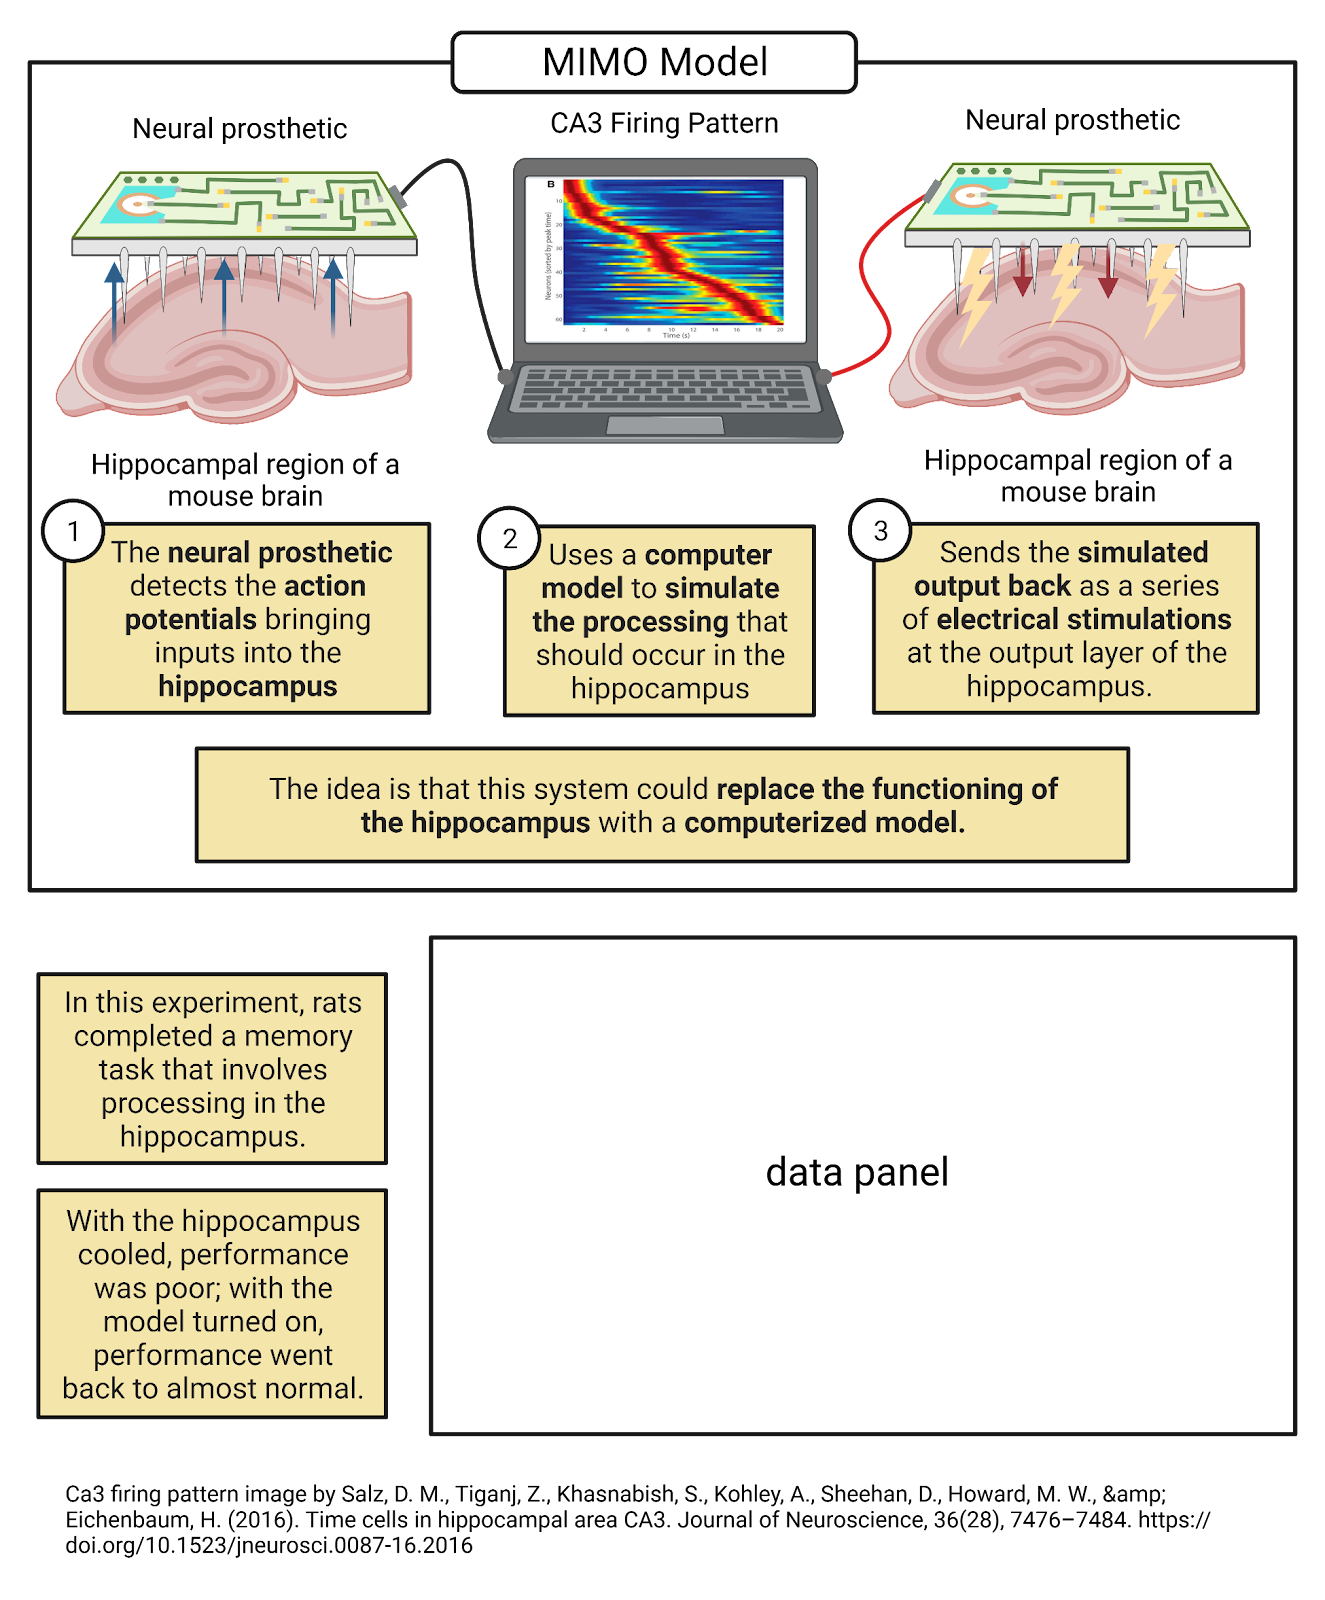
\includegraphics[width=0.8\linewidth]{images/ch02/02_09} 

}

\caption{Computational neuroscientists have developed an artificial hippocampus.}(\#fig:ch02_09)
\end{figure}

\hypertarget{topic-summary-1}{%
\subsection{Topic summary}\label{topic-summary-1}}

Communication between neurons allows them to form circuits that can generate complex rhythms and behaviors. In the \emph{Tritonia} swim network, attack from a predator activates sensory neurons as well as inhibitory feedback that generates cycles of contraction and relaxation that ``swim'' the animal away from danger. This example typifies some of the key properties of neural networks: they are highly efficient, operate in parallel, feature extensive and complex forms of feedback, but are susceptible to malfunction from either too much or too little activity. The field of computational neuroscience explores mathematical models of neurons that can be simulated on a computer; this field is succeeding in producing artificial networks that can mimic many of the remarkable behaviors produced by animal nervous systems.

\textbf{Key Terms}

\begin{itemize}
\item
  Rhythm
\item
  Feedback
\item
  Parallel processing
\item
  Model
\item
  Computational neuroscience
\item
  Simulation
\item
  Abstraction
\item
  Neural prosthetic
\end{itemize}

\textbf{References and works cited}

\begin{itemize}
\item
  Balasubramanian V (2021) Brain power. Proc Natl Acad Sci 118 Available at: \url{https://pnas.org/doi/full/10.1073/pnas.2107022118}.
\item
  Berger TW, Hampson RE, Song D, Goonawardena A, Marmarelis VZ, Deadwyler S a (2011) A cortical neural prosthesis for restoring and enhancing memory. J Neural Eng 8:046017 Available at: \url{http://www.ncbi.nlm.nih.gov/pubmed/21677369} {[}Accessed June 17, 2011{]}.
\item
  Berger TW, Song D, Chan RHM, Marmarelis VZ, LaCoss J, Wills J, Hampson RE, Deadwyler SA, Granacki JJ (2012) A Hippocampal Cognitive Prosthesis: Multi-Input, Multi-Output Nonlinear Modeling and VLSI Implementation. IEEE Trans Neural Syst Rehabil Eng 20:198--211.
\item
  Brown GD (1998) Nonassociative learning processes affecting swimming probability in the seaslug Tritonia diomedea: habituation, sensitization and inhibition. Behav Brain Res 95:151--165 Available at: \url{http://www.ncbi.nlm.nih.gov/pubmed/9806436}.
\item
  Calin-Jageman RJ, Tunstall MJ, Mensh BD, Katz PS, Frost WN (2007) Parameter space analysis suggests multi-site plasticity contributes to motor pattern initiation in Tritonia. J Neurophysiol 98:2382--2398 Available at: \url{http://www.ncbi.nlm.nih.gov/pubmed/17652417}.
\item
  Deadwyler SA, Berger TW, Sweatt AJ, Song D, Chan RHM, Opris I, Gerhardt GA, Marmarelis VZ, Hampson RE (2013) Donor/recipient enhancement of memory in rat hippocampus. Front Syst Neurosci 7 Available at: \url{http://journal.frontiersin.org/article/10.3389/fnsys.2013.00120/abstract}.
\item
  Getting PA (1983) Mechanisms of pattern generation underlying swimming in Tritonia. II. Network reconstruction. J Neurophysiol 49:1017--1035 Available at: \url{https://www.physiology.org/doi/10.1152/jn.1983.49.4.1017}.
\item
  Hampson RE, Song D, Robinson BS, Fetterhoff D, Dakos AS, Roeder BM, She X, Wicks RT, Witcher MR, Couture DE, Laxton AW, Munger-Clary H, Popli G, Sollman MJ, Whitlow CT, Marmarelis VZ, Berger TW, Deadwyler SA (2018) Developing a hippocampal neural prosthetic to facilitate human memory encoding and recall. J Neural Eng 15:036014 Available at: \url{https://iopscience.iop.org/article/10.1088/1741-2552/aaaed7}.
\item
  Herculano-Houzel S (2012) The remarkable, yet not extraordinary, human brain as a scaled-up primate brain and its associated cost. Proc Natl Acad Sci U S A 109:10661--10668.
\item
  Hoppe T (1998) An evaluation of the role of synaptic depression at afferent synapses in habituation of the escape swim response of Tritonia diomedea.
\item
  Katz PS, Frost WN (1997) Removal of Spike Frequency Adaptation via Neuromodulation Intrinsic to the Tritonia Escape Swim Central Pattern Generator. J Neurosci 17:7703--7713 Available at: \url{https://www.jneurosci.org/lookup/doi/10.1523/JNEUROSCI.17-20-07703.1997}.
\item
  Willows AOD, Hoyle G (1969) Neuronal Network Triggering a Fixed Action Pattern. Science (80- ) 166:1549--1551 Available at: \url{https://www.science.org/doi/10.1126/science.166.3912.1549}.
\end{itemize}

\hypertarget{neurophysiology-bioelectricity}{%
\section{Principles of bioelectricity}\label{neurophysiology-bioelectricity}}

\textbf{Learning objectives}

By the end of this section, students will be able to:

\begin{itemize}
\item
  Objective 1: Define fundamental concepts of electricity (current (I), conductance (G), and electrical potential (V)) and the inter-relationships between them defined by Ohm's law (e.g.~I = GV)
\item
  Objective 2: List the 4 main electrolytes (K+, Na+, Cl-, and Ca++) that underlie most electrical currents in neurons and describe how the movement of each electrolyte is determined both by electrostatic force (opposites attract; likes repel) and diffusion (movement from high to low concentration).
\item
  Objective 3: Describe the major players in controlling electrolyte movement: 1) the cell membrane, which has a high conductance that blocks electrolyte movement, enabling each neuron to store up charges to maintain a membrane potential, 2) ion pumps, which use energy to push Na+, Ca++, and Cl- out of neurons and K+ into neurons to maintain concentration-gradient batteries for each electrolyte, and 3) ion channels, which provide passive but selective pathways for electrolytes, generating currents that depend on the number of open channels and the driving force for each ion.
\end{itemize}

In a chemistry lab at Harvard university, a team of researchers led by Adam Cohen is developing new ways to `listen in' on the electrical signals in neurons (Kralj et al., 2012). One approach is the development of **voltage-sensitive fluorescent proteins\_, \_**genetically-engineered proteins that give off fluorescent light based on their electrical environment (Image 2:10). When expressed in neurons, these proteins can translate the electrical signals in neurons into light that can be captured on a specialized camera. To test their work, the researchers carefully culture neurons, growing them in a dish where they can provide the nutrients the neurons need to survive plus the instructions for assembling the new voltage-sensitive proteins the lab has developed. One neuron is then placed under a fluorescent microscope equipped with a camera that can record 100,000 images per second. Adjusting the knobs on the microscope, the researchers bring a single neuron into focus. Then, they work intensely to keep the neuron healthy and the recording stable.

\begin{figure}

{\centering 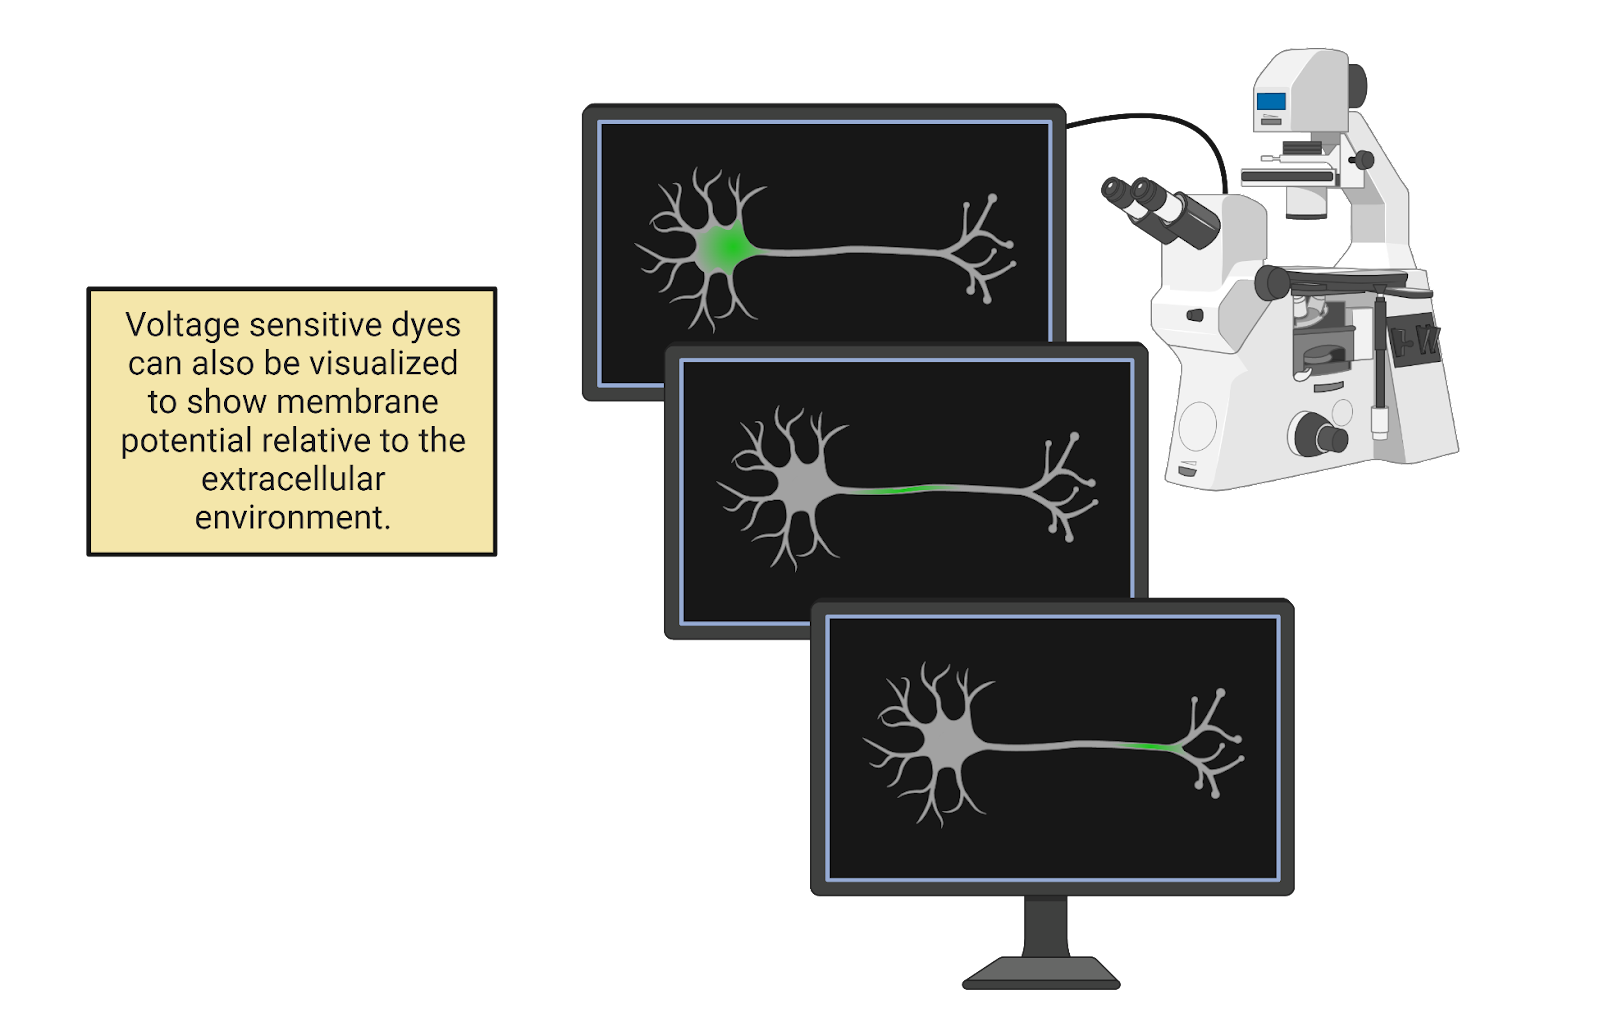
\includegraphics[width=0.8\linewidth]{images/ch02/02_10} 

}

\caption{Voltage-sensitive flourescent proteins show how action potentials spread rapidly through a neuron.}(\#fig:ch02_10)
\end{figure}

After several hours recording with the microscope (and several days processing all the data), the researchers assemble a remarkable video. Check it out on here:\url{http://cohenweb.rc.fas.harvard.edu/}. In the video, you can ``see'' the neuron generating action potentials. At first, there is no fluorescent signal in the neuron; it is at its negative resting potential and this does not activate the dye. Suddenly, though, we see a tiny glimmer of electrical change: the cell body has become positively charged! This region of positive charge then spreads out, traveling through every stem and branch of the neuron's complex axonal tree. As quickly as it spreads, the action potential also fades, so the whole neuron is quickly back to its normal negative resting potential. The video is slowed down, but the timer on the top-left of the screen shows that the rise-and-fall of the action potential occurs very quickly, in less than 1 millisecond. If we graph the intensity of the dye over time, we see that each branch of the axon experiences this rapid ``spike'' in voltage, flipping from negative to positive and back again.

Watching this video, you are witnessing action potential \textbf{propagation}, the spreading of an action potential that relays information from one end of a neuron to another at great speed. But, you may be wondering: what, exactly, am I seeing? What does it mean to say that an action potential is \emph{electrical}? Is the electricity in a neuron the same as what is coursing through your cell phone or laptop? And if so, how do neurons generate their own electricity? To answer these questions, we first need to get our footing with some fundamental concepts of electricity. Then we'll see how **ion pumps\_ \emph{\textbf{and }ion channels} \emph{\textbf{enable neurons to generate signals via the controlled movement of four }electrolytes} \_**found in your cellular fluids: sodium, potassium, chloride, and calcium.

\hypertarget{fundamentals-of-electricity-charge-current-conductance-and-potential.}{%
\subsection{Fundamentals of electricity: Charge, current, conductance, and potential.}\label{fundamentals-of-electricity-charge-current-conductance-and-potential.}}

Electricity is the movement of \textbf{charge}. Charge is a fundamental property of sub-atomic particles: electrons have a negative charge; protons have a positive charge. For reasons even physicists don't completely understand, charges exert force on one another: opposites attract and likes repel (Image 2.11).

\begin{figure}

{\centering 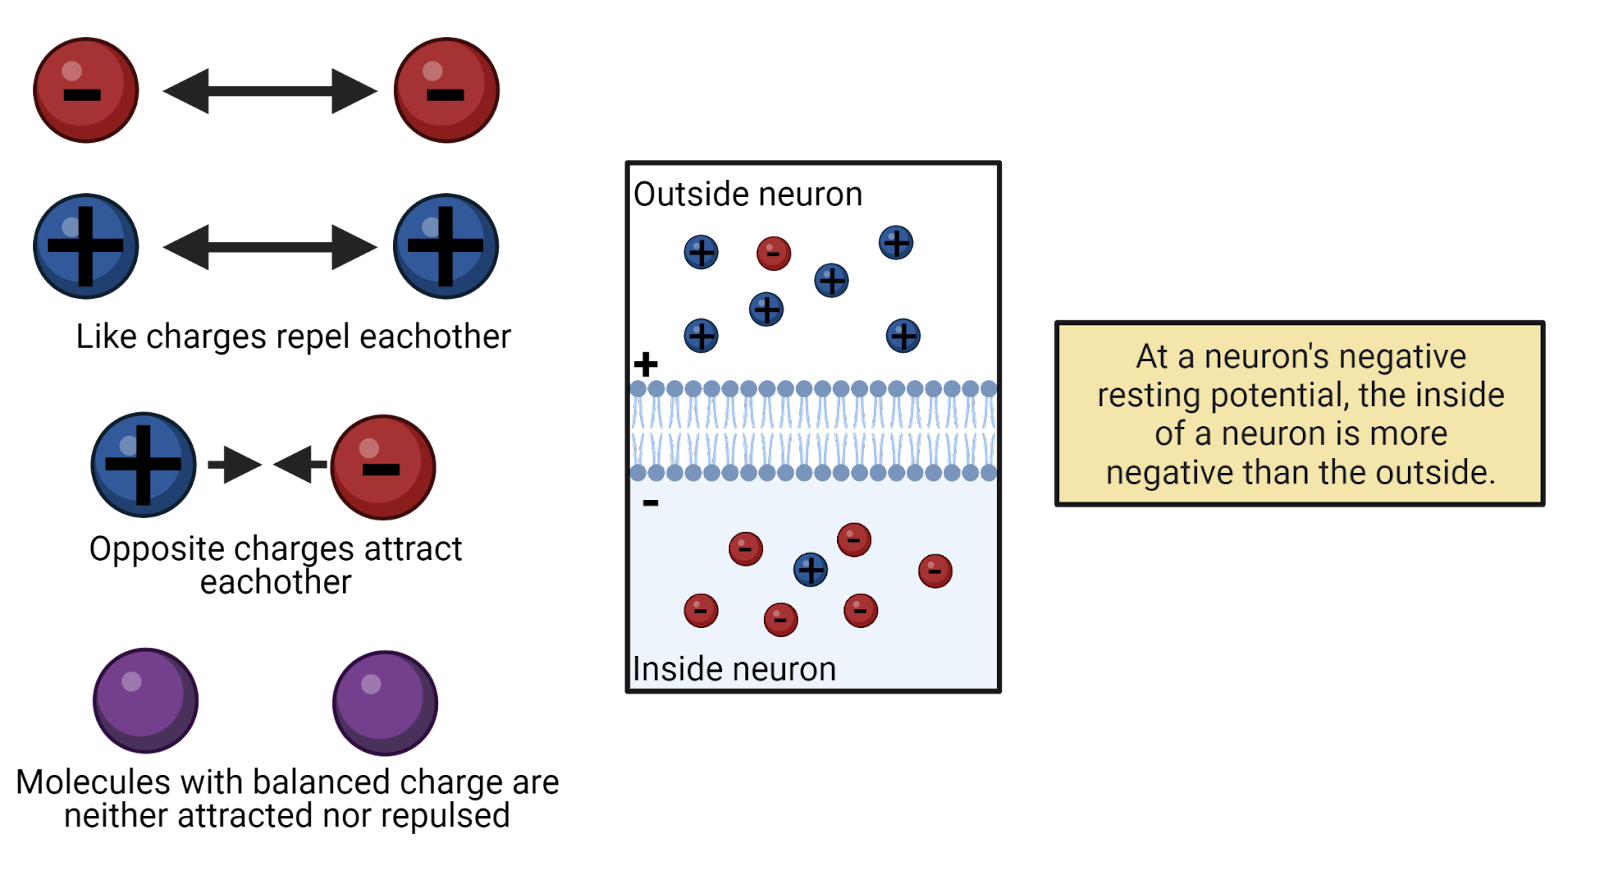
\includegraphics[width=0.8\linewidth]{images/ch02/02_11} 

}

\caption{Electrostatic force.}(\#fig:ch02_11)
\end{figure}

If a molecule has equal numbers of protons and electrons, then its \emph{net charge} is 0 and the molecule is electrically \emph{neutral}. When a molecule has an imbalance of protons and electrons, though, it is said to \emph{carry a charge}, meaning that it has a net positive or negative charge that will exert \textbf{electrostatic force} on other charged particles. We call a charged particle an \textbf{ion}. In physics, charge is given the symbol \emph{Q}. Charge is measured in \textbf{coulombs}.

If you've ever played with magnets you've been able to feel electrostatic forces at work. Hold the positive pole of a magnet near the negative pole of another and you can feel the \emph{attractive force} between opposite charges. Flip one of the magnets around and try to push the positive poles together and you can feel the \emph{repulsive force} between like charges. The same repulsion occurs if you try to push the negative poles of two magnets together. You've probably noticed that to feel these forces you need to hold the magnets close together. That's because electrostatic force depends on the distance between charges, growing exponentially stronger as the distance decreases, and exponentially weaker as the distance increases (something you may have learned in physics as Coulomb's law).

Forces induce movement. Because of the electrostatic forces between them, ions move towards their opposites and away from their likes, if they can. The movement of ions is an electrical **current\_ \emph{\textbf{which does \emph{work}. It is this \emph{movement} of charge that we call electricity. Anywhere we see work being done by electricity there must be a current flowing: a light bulb glows as electrical current flows through its light-emitting diode, your laptop responds to your commands as electrical current surges through its transistors. In physics, the symbol for current is \emph{I}. We measure electrical currents in }amperes** (often shortened to a\_mps}), which tells us about rate at which charge is flowing (number of Coulombs of charge per second).

When an electrical current flows, the path it takes can impede the movement of the ions or it can allow an easy passage. We call this \textbf{conductance}. Physicists use the symbol \emph{G} for conductance, which is measured in \textbf{seimens}. For example, water has a fairly high conductance, meaning that charged particles in water can rapidly respond to electrostatic forces, moving to disperse from their likes and to unite with their opposites. Cell membranes, on the other hand, have very low conductance, and act as **insulator\_. \_**(If you've had a physics class that discussed \emph{resistance} rather than conductance, don't panic: these are the same idea but expressed from different perspectives. Conductance is a measure of how \emph{easy} it is to move charge; resistance is a measure of how \emph{difficult} it is to move charge. You can convert back and forth between conductance and resistance: G = 1/R; R = 1/G.)

By acting as an insulator, cell membranes can hold electrostatic forces ``in check'', holding ions in place even if electrostatic forces are pushing to move them. We call this pent-up energy \textbf{electrical potential}; it is a push or pressure just waiting to generate a current should a conductive pathway become available. In physics, the symbol for electrical potential is V, and it is measured in volts. You'll often hear electrical potential referred to as \emph{voltage}. Technically, this mixes up the unit (volt) with the concept (electrical potential), but the term has become so popular that we can just accept voltage as a synonym for electrical potential.

Current, conductance, and potential are inter-related: I = G * V (Image 2.12). This relationship is known as \textbf{Ohm's law}. This means the electrical current that flows in a system is determined by the product of the conductance (how easy it is for charge to move) and the potential (how much pressure there is for charge to move). You can use algebra to re-arrange Ohm's law to solve for different electrical concepts (for example, V = I/G is \emph{also} Ohm's law); this is because in all of its forms Ohm's law expresses the idea that potential, conductance, and current are inter-related in such a way that knowing any two of these values instantly tells you the third.

\begin{figure}

{\centering 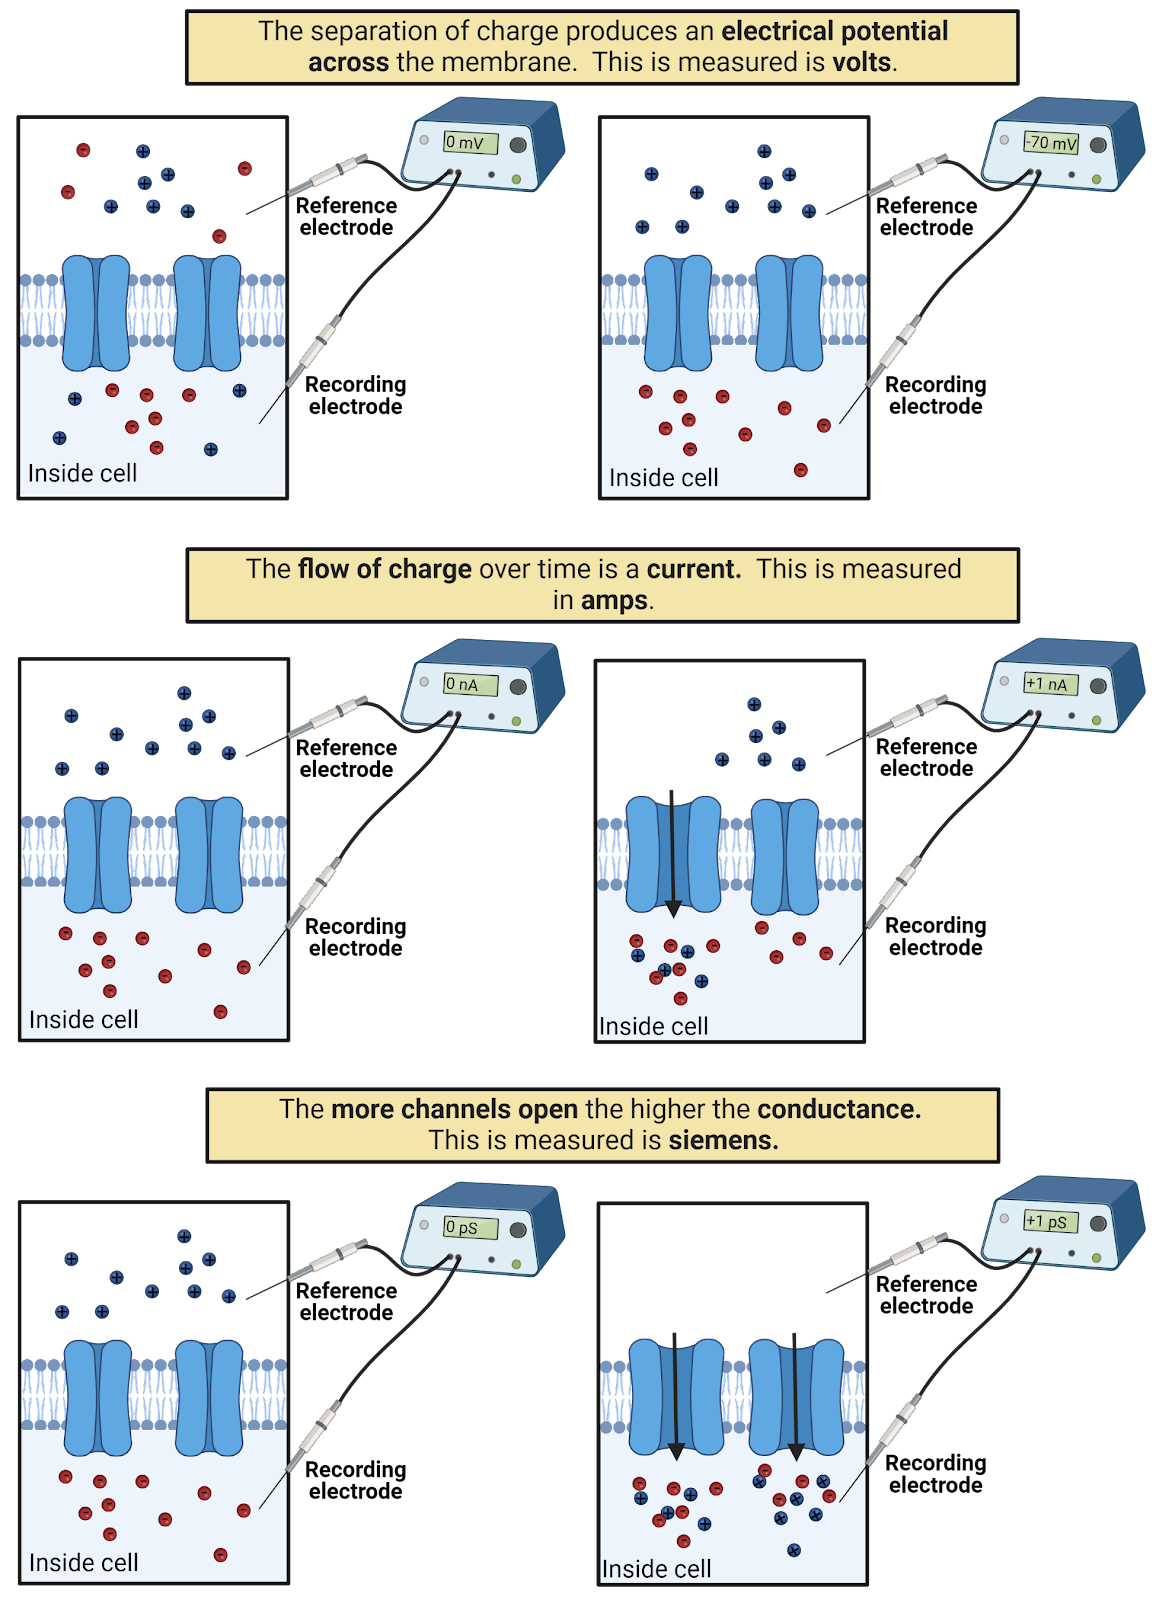
\includegraphics[width=0.8\linewidth]{images/ch02/02_12} 

}

\caption{Ohm's Law.}(\#fig:ch02_12)
\end{figure}

\hypertarget{electrical-signaling-in-neurons-involves-changes-in-potential-and-can-be-measured-with-a-voltmeter.}{%
\subsection{Electrical signaling in neurons involves changes in potential and can be measured with a voltmeter.}\label{electrical-signaling-in-neurons-involves-changes-in-potential-and-can-be-measured-with-a-voltmeter.}}

Electrical signaling in neurons involves changes in current, conductance, and potential. The easiest of these to measure in neurons, though, is potential. Because of this, scientists first characterized and named the electrical signals in neurons in terms of electrical potential: the resting \emph{potential}, excitatory and inhibitory post-synaptic \emph{potentials}, and the action \emph{potential}.

We can measure a neuron's \textbf{membrane potential }(\emph{VM}) by connecting it to a \textbf{voltmeter}, a device for measuring electrical potential (Image 2.13). All that is needed is a voltmeter and two wires, or \textbf{electrodes}. For neurons, this usually means placing one wire, called the \emph{recording electrode}, \emph{inside} the neuron, and a second wire, called a \emph{reference electrode}, \emph{outside} the neuron. The voltmeter measures the electrical potential between these two points, indicating the difference in charge across the neuron's membrane, it's membrane potential. A negative membrane potential (as a neuron has at rest) indicates the inside of the neuron has a net negative charge relative to the outside of the neuron. A positive membrane potential (as a neuron has at the peak of an action potential) indicates the neuron has a net positive charge relative to the outside. A membrane potential of 0 volts indicates no imbalance of charge: the neuron is electrically neutral relative to the reference electrode.

\begin{figure}

{\centering 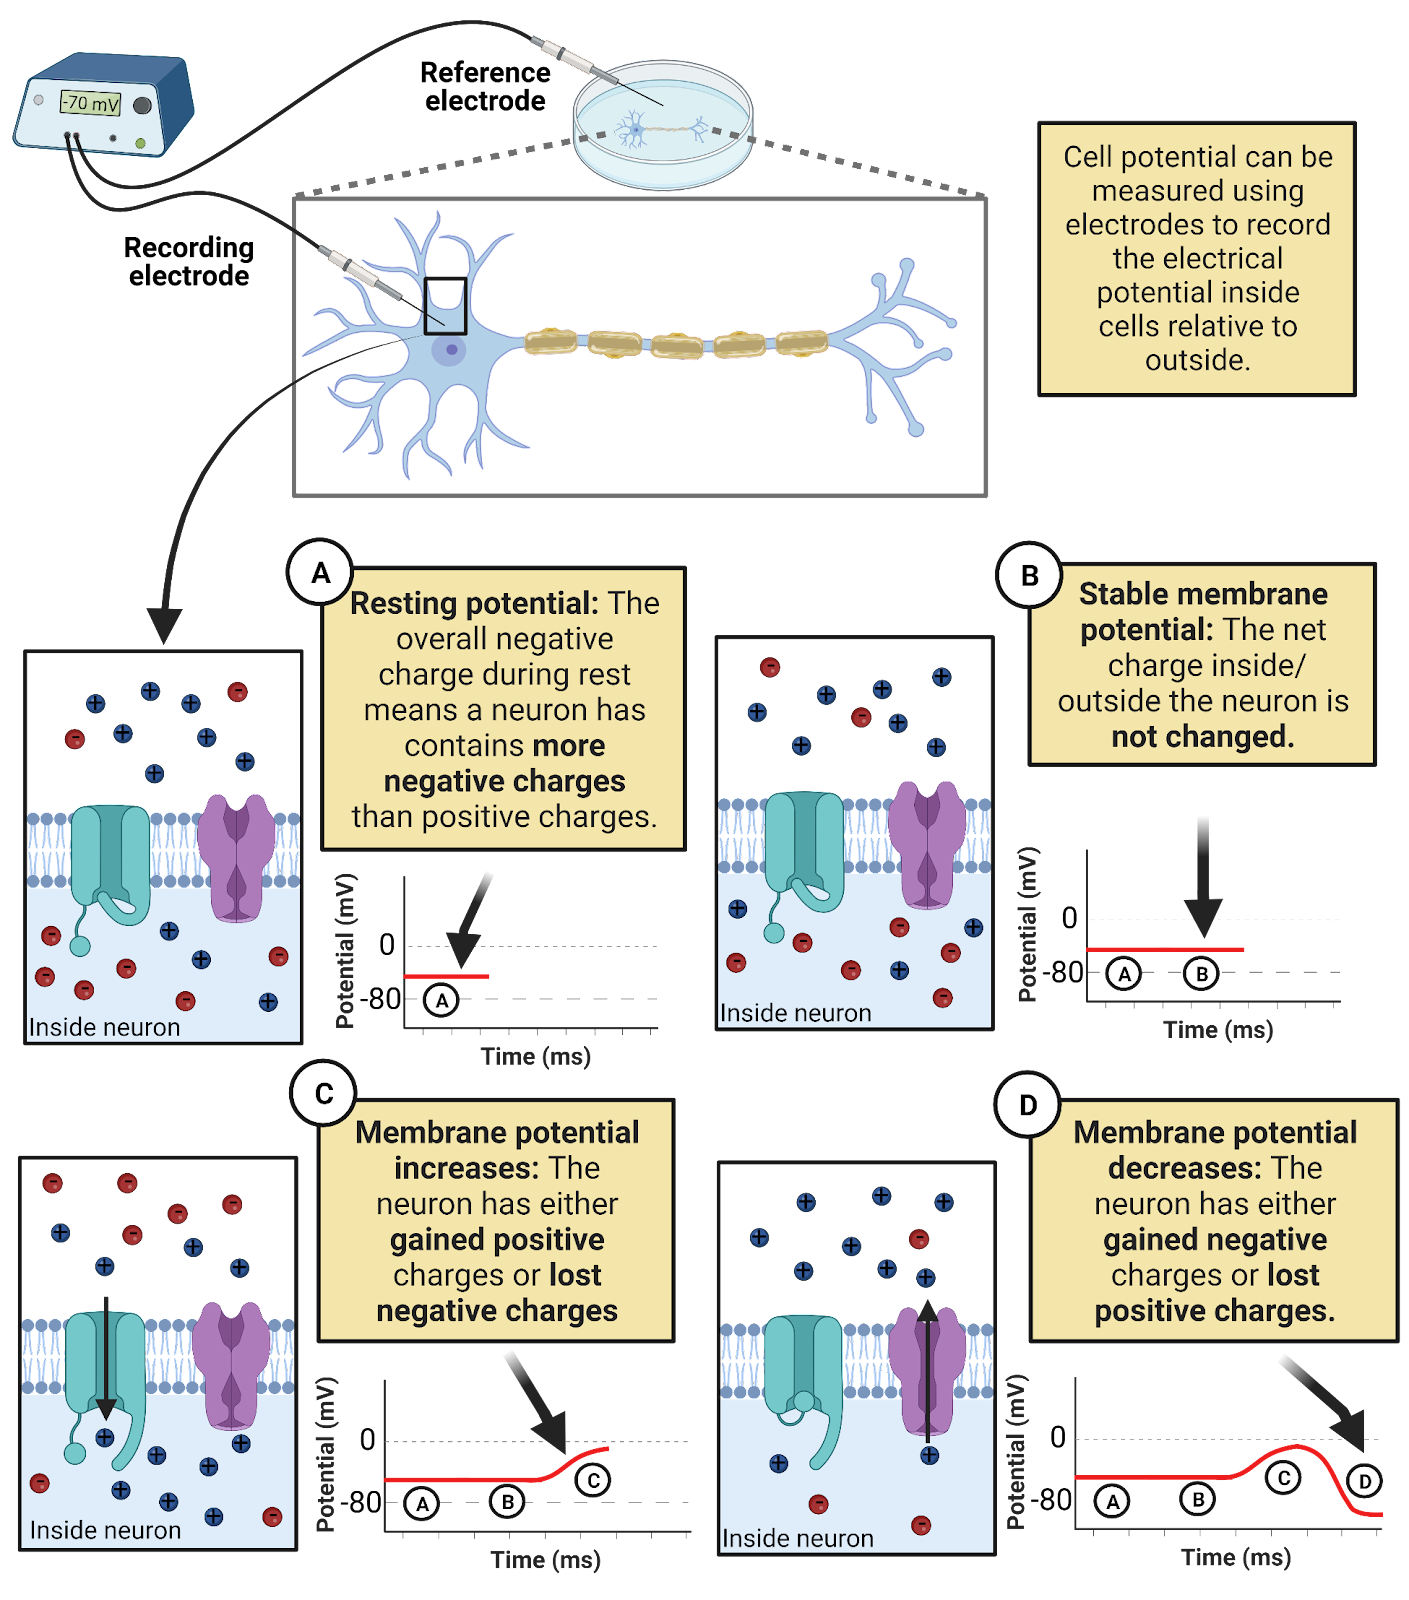
\includegraphics[width=0.8\linewidth]{images/ch02/02_13} 

}

\caption{Measuring changes in neuronal membrane potential with a voltmeter.}(\#fig:ch02_13)
\end{figure}

In some ways, \textbf{neurophysiology}, the recording of electrical signals from neurons, is no different than when a mechanic checks the charge on your car's battery. There are some huge technical difficulties, though, including the challenge of trying to place the tip of an electrode \emph{inside} a microscopic neuron (!). The methods section in this book explains some of the specialized equipment that is used to make neurophysiology possible.

When you hook a voltmeter up to a car battery, you will observe a stable potential (unless something has gone very wrong). In contrast, membrane potential in neurons is highly dynamic: it is negative at rest, becomes slightly more negative during an IPSP, becomes slightly more positive during an EPSP, and flips to positive and back to negative during action potentials. Because of this, \textbf{we graph membrane potential as a function of time}. When a neuron's membrane potential increases, we know that a current has flowed that either brought positive charge into the neuron or that removed negative charge. When a neuron's membrane potential decreases, we know that a current has flowed that either brought negative charge into the neuron or removed positive charge. When a neuron has a stable membrane potential, we know that that there is no net current, maintaining the neuron's current charge.

Another complexity of neural electricity is that membrane potential varies over the length of a neuron's dendrites and axons. EPSPs and IPSPs alter membrane potential right at the synapse. Action potentials travel down the axon, with one segment flipping to a positive potential while segments just ahead are still at their negative resting potential. Thus, we have to keep track of not only how membrane potential changes over time but also \emph{where} membrane potential is changing.

Voltage-sensitive dyes enable us to measure potential along an entire neuron at once, so we can ``see'' the locations of different signals and how they spread. In contrast, a voltmeter can only measure membrane potential at the exact location of the recording electrode. Because of this, the first recordings of action potentials captured only the up and down of electrical potential at a single point, showing up as a ``spike'' in the membrane potential recording. The \emph{spread} of an action potential had to be deduced from systematically moving the electrode along the length of the axon. When you see an action potential ``spike'' from a voltmeter, try to keep in mind that it is just a limited view of what is actually an electrical wave that spreads through the axon.

\hypertarget{electrical-currents-in-neurons-are-the-movement-of-four-electrolytes-dissolved-in-your-cellular-fluids-na-k-cl--and-ca.}{%
\subsection{Electrical currents in neurons are the movement of four electrolytes dissolved in your cellular fluids: Na+, K+, Cl-, and Ca++.}\label{electrical-currents-in-neurons-are-the-movement-of-four-electrolytes-dissolved-in-your-cellular-fluids-na-k-cl--and-ca.}}

What are the moving charges that generate electrical currents in neurons? Trace minerals dissolved in your intracellular and extracellular fluids (Image 2.14). Nearly all electrical signaling in neurons is due to the movement of just 4 types of minerals: sodium (chemical symbol Na+), potassium (chemical symbol K+), calcium (Ca++) and chloride (Cl-). Notice the positive and negative symbols next to the chemical symbols. That is because each is not only a mineral but also an \textbf{electrolyte}, something that dissolves into water as an \textbf{ion}, a charge-carrying molecule. For example, sodium is represented as Na+ because as a \textbf{solute} (a substance dissolved in water) each molecule of sodium has 11 positive protons but only 10 negative electrons, yielding a net charge of +1. Chloride molecules, on the other hand, have 17 protons and 18 electrons when dissolved in water, a net charge of -1. Calcium has a double-positive symbol because calcium molecules in water have 18 protons but only 16 electrons.

\begin{figure}

{\centering 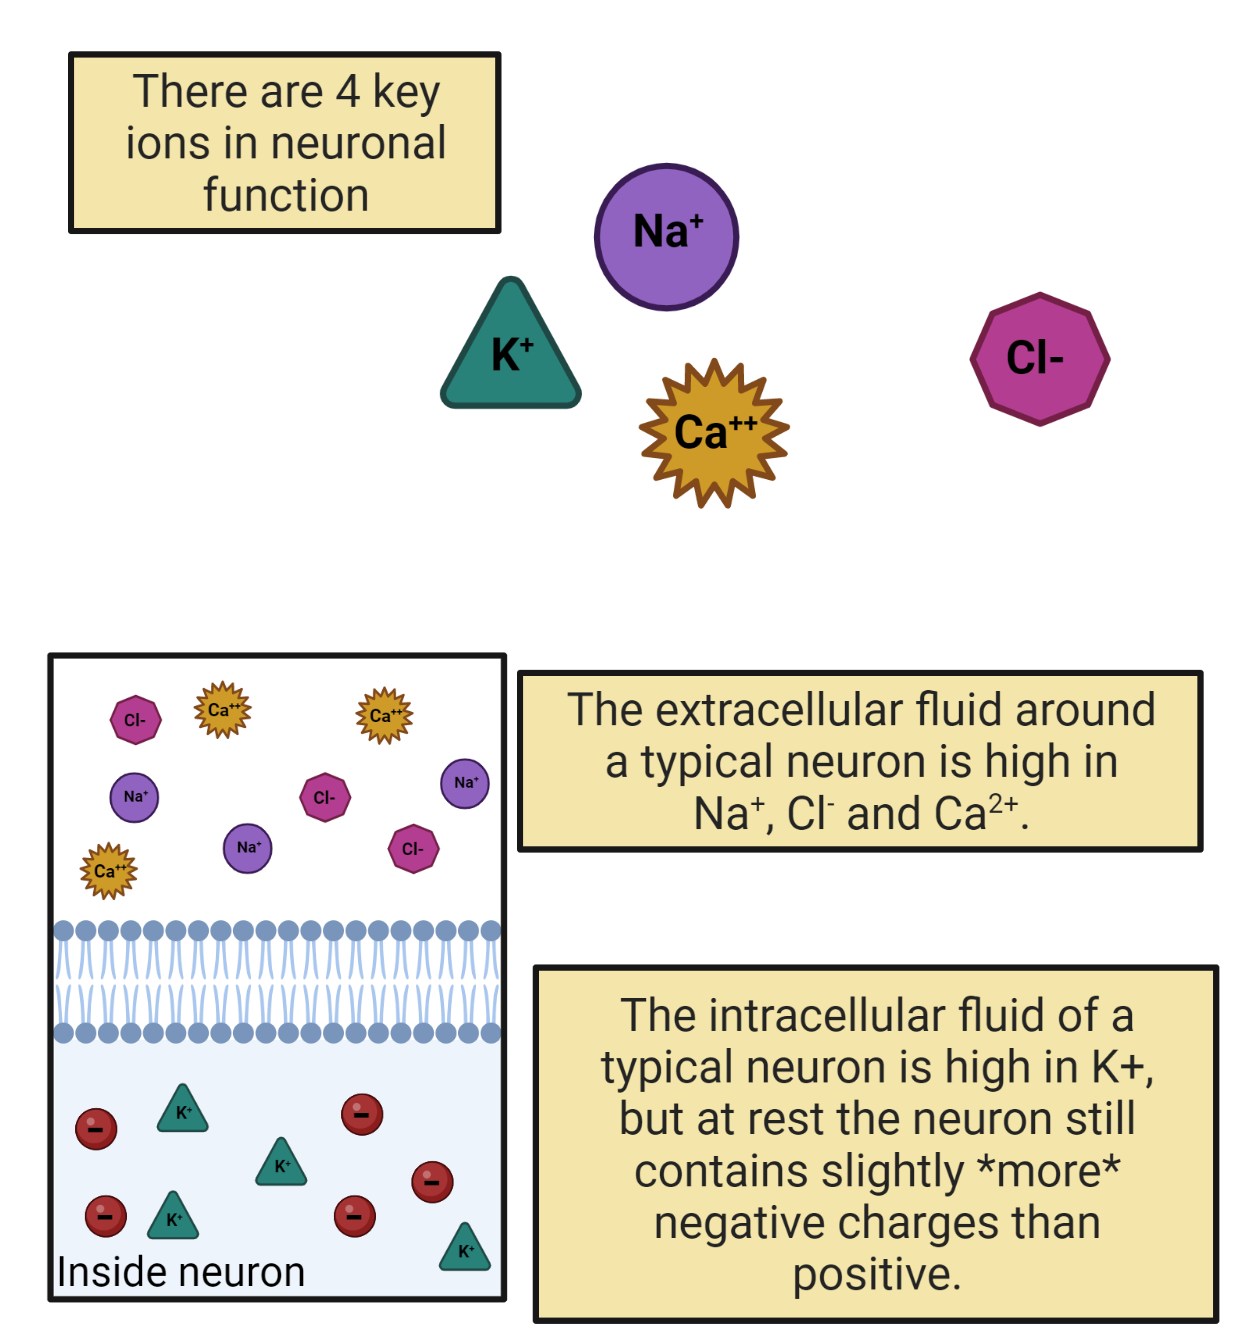
\includegraphics[width=0.8\linewidth]{images/ch02/02_14} 

}

\caption{Key electrolytes for neuronal signaling.}(\#fig:ch02_14)
\end{figure}

Because electrolytes dissolved in water carry a charge, their movement \emph{is} an electrical current. \textbf{It is the movement of Na+, K+, Cl-, and Ca++ into and out of neurons that we observe as electrical signals in neurons.} The resting potential? It is due to K+ shuttling into and out of a neuron to keep the membrane at a negative potential. Action potentials? They are due to a chain reaction of Na+ entering a neuron followed by K+ departing. Inhibition? That's just a temporary entry of Cl- into a neuron. Excitation? Each EPSP is a brief entry of Na+ and/or, Ca++. Electrical signaling in neurons is just the careful gatekeeping of these dissolved electrolytes.

In the next section, we'll examine the pressures that can drive this movement: electrostatic force and diffusion. Before we move on, you might be wondering: where do electrolytes come from? The K+, Na+, Cl-, and Ca++ dissolved in your cellular fluids come from your diet. For example, bananas are loaded with K+. You lose electrolytes in your urine and in your sweat, so you need daily intake from your diet to keep the proper balance of electrolytes in your body. That's why sports drinks are always promising to ``replenish your electrolytes''---they are selling you sugar water supplemented with a few milligrams of these basic minerals (though some leave out the calcium). Electrolytes are essential not only for generating neural electricity, but for nearly all cellular processes, including transcription and translation. This reflects the ancient origins of life in the Earth's oceans: the Na+, K+, Cl-, and Ca++ dissolved in your cellular fluids are the same trace minerals found in salt water and are ubiquitous (ever-present) in all cellular forms of life. At the dawn of the animal kingdom, new mechanisms evolved to harness electrolytes for a new function: neural signaling.

\hypertarget{electrolytes-are-moved-by-electrostatic-force-and-diffusion-but-their-movement-is-blocked-by-the-cell-membrane.}{%
\subsection{Electrolytes are moved by electrostatic force and diffusion but their movement is blocked by the cell membrane.}\label{electrolytes-are-moved-by-electrostatic-force-and-diffusion-but-their-movement-is-blocked-by-the-cell-membrane.}}

What \emph{moves} the molecules of electrolytes dissolved in your cellular fluids? Two things: electrostatic force and \textbf{diffusion }(Image 2.15).

We've already discussed electrostatic force. Every molecule of Na+, K+, Ca++, and Cl- dissolved in your cellular fluids carries a charge. Because of this, each is subject to electrostatic forces that push them towards their opposites and away from their likes.

Because they are dissolved in water, your electrolytes also diffuse, spreading out, as much as possible, towards equal concentration. The rules of diffusion are simple: when possible, solutes will always move down a \textbf{concentration gradient}, spreading from a region of high concentration to a region of low concentration, moving towards an equilibrium of equal concentration. The steeper the concentration gradient (the more different the concentrations between regions) the stronger the entropic push of diffusion.

\begin{figure}

{\centering 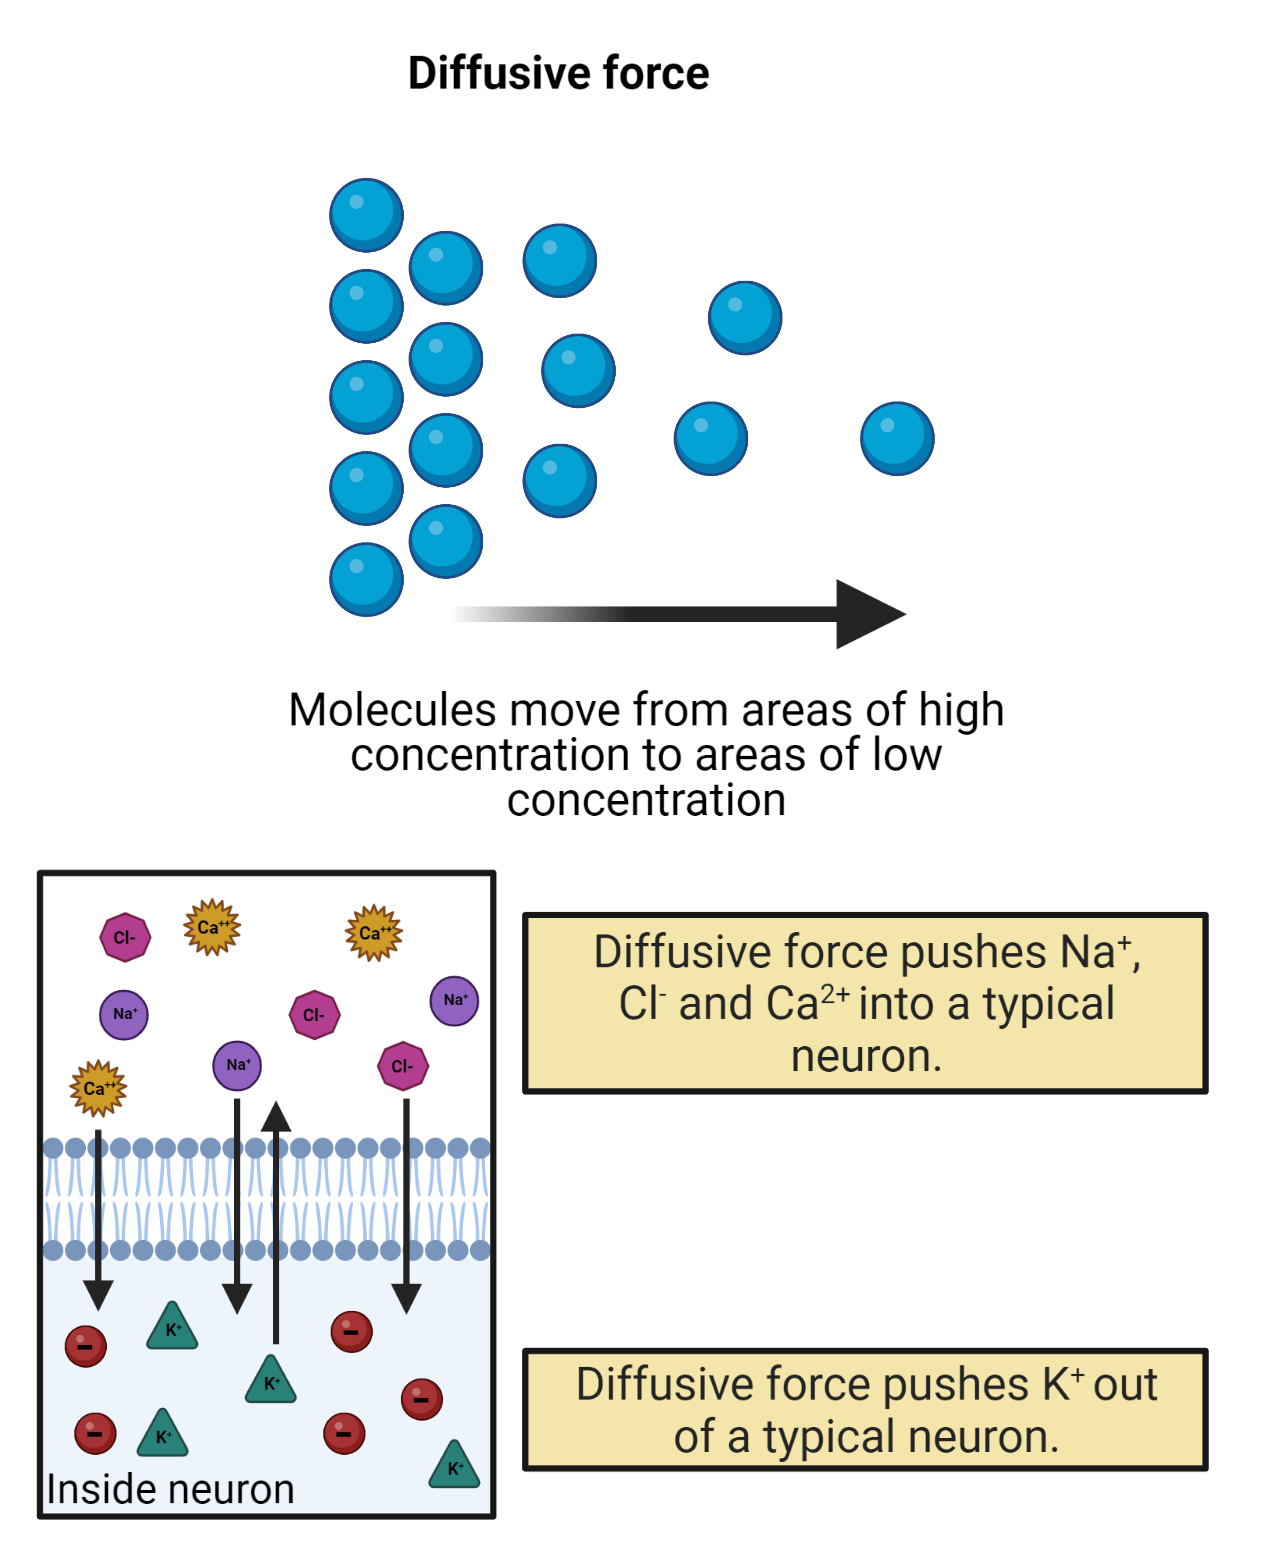
\includegraphics[width=0.8\linewidth]{images/ch02/02_15} 

}

\caption{Diffusion.}(\#fig:ch02_15)
\end{figure}

Diffusion and electrostatic force sum and together can produce strong pressure on ions to move. Water has a high conductance, so diffusion and electrostatic force can easily move ions around inside your cellular fluids. The cell membrane, on the other hand, has a low conductance; ions cannot move \emph{directly} through the cell membrane. This is because each molecule of dissolved electrolyte becomes surrounded by a shell of water molecules, called a \textbf{sphere of hydration}. This shell is strongly repelled by the lipid bilayer structure of the cell membrane. Thus, a molecule of K+ inside a neuron cannot \emph{directly} leave the neuron, even if electrostatic force and diffusion are pushing it to do so. If you're a LOTR fan, you could say that the cell membrane is the Gandalf of neural signaling (``You shall not pass!''). Less funny, but more accurately, we can say that the cell membrane enables cells to act as \textbf{capacitors}, containers for electrical charge. That is, each stored charge is an electrical potential, as it is drawn towards its opposite across the membrane but can't actually pass to them.

Physics shows how to calculate the electrical potential produced by charge stored in a capacitor:

VM = Q/C

This just means that a neuron has a membrane potential (\emph{VM}) based on how much charge is being held back by its membrane (\emph{Q}) and also its **capacitance\_ \_**(\emph{C}). A neuron's capacitance has to do with both its size (the bigger the neuron the higher its capacitance because the charges can spread out more and therefore have less electrostatic pressure to leave) and the thickness of the membrane (the thicker the membrane the higher the neuron's capacitance, because the electrostatic pressure across the membrane grows weaker with distance). If you haven't had a physics class yet, the idea of capacitance might leave you cold. But what should make sense is that the more charge stored up in a neuron and blocked from leaving by the membrane, the stronger that neuron's membrane potential (the more potential energy there is to move those ions should a pathway through the membrane become available).

Recall that the movement of charge is a current. So it can also be helpful to express the change in membrane potential as a function of current:

\begin{verbatim}
        dV<sub>M</sub>/dt = I/C
\end{verbatim}

Which just says that currents passing into or out of a neuron change its membrane potential (because they change the amount of charge being held back by the membrane).

Putting this together, we see that membranes are a strong barrier to the movement of electrolytes, allowing neurons to store charges to create a membrane potential. If the membrane blocks electrolyte movement, how do they travel into and out of neurons, generating the currents that carry signals in neurons? All ion traffic occurs via \emph{transmembrane proteins}---amino acid machines that stick through the membrane. In the next sections we'll discuss two families of proteins that control the movement of electrolytes: ion pumps and ion channels.

\hypertarget{ion-pumps-create-concentration-gradient-batteries-concentrating-k-inside-neurons-and-na-ca-and-cl--outside.}{%
\subsection{Ion pumps create concentration-gradient batteries, concentrating K+ inside neurons and Na+, Ca++, and Cl- outside.}\label{ion-pumps-create-concentration-gradient-batteries-concentrating-k-inside-neurons-and-na-ca-and-cl--outside.}}

For your cell phone to work, it needs a battery, something that can generate a steady electrical potential to push electrical currents through the circuits in your phone. Neurons also have batteries. They use \textbf{ion pumps} to create **concentration gradients\_ \_\textbf{of the electrolytes found in your cellular fluids (Image 2.16). K+ is pushed into cells, concentrating it in the intracellular fluid; Na+, Cl-, and Ca++ are pushed out of cells, concentrating them in the extracellular fluid. These concentration gradients are chemical }batteries**, giving each ion a distinct ``push'' from diffusion towards an electrical potential (Table 2.01).

\begin{figure}

{\centering 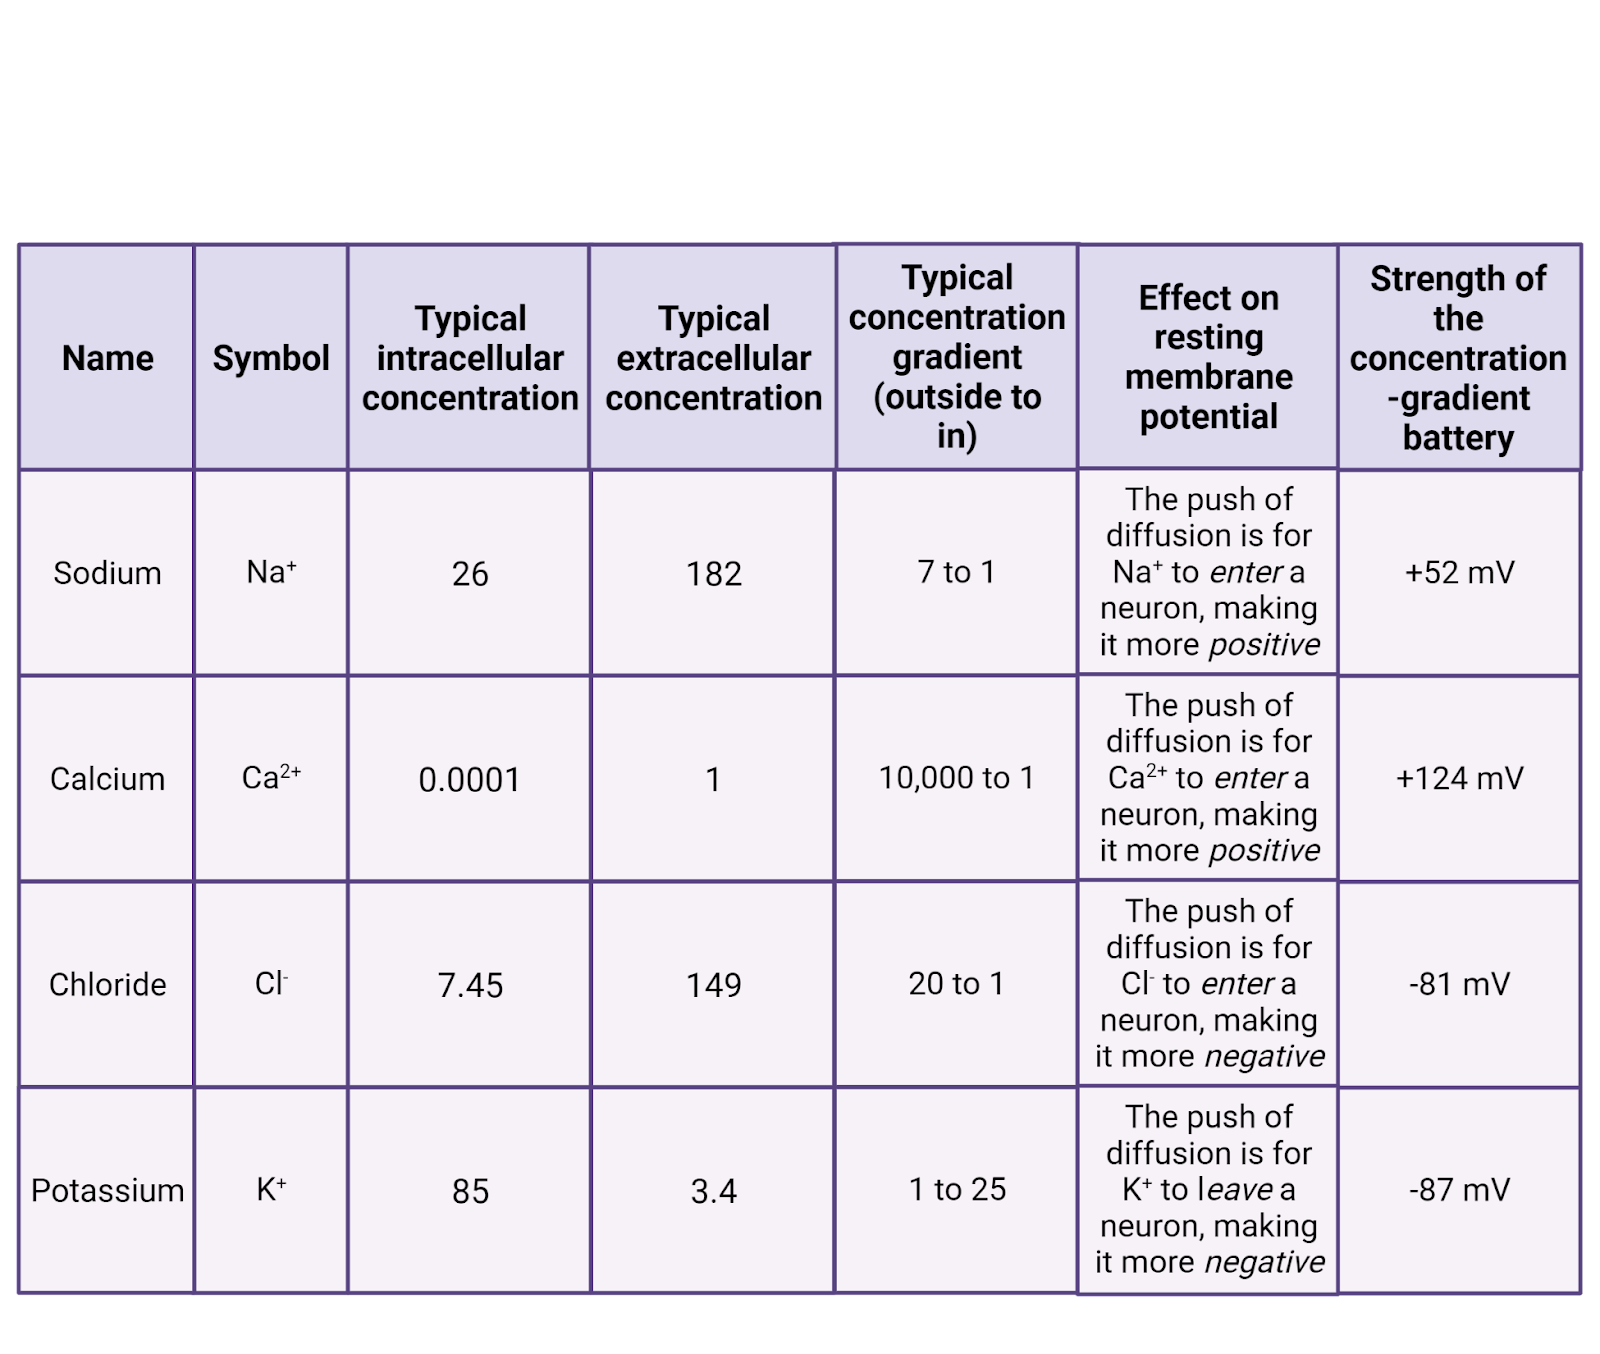
\includegraphics[width=0.8\linewidth]{images/ch02/table_02_02} 

}

\caption{Electrolytes involved in neural signalling.}(\#fig:table_ch02_01)
\end{figure}

Ion pumps are proteins that stick through the membrane. They use energy to actively transport ions across the cell membrane. Ion pumps work \emph{against} diffusion, moving ions across the cell membrane so that they become \emph{more} concentrated rather than less. This builds a pressure of diffusion for each ion.

All the cells in your body express ion pumps. For example, one type of pump pushes Ca++ out of the cell. Once pushed outside the cell, Ca++ cannot directly re-enter (because Ca++ cannot pass directly through the cell membrane). Because of the operation of Ca++ pumps and the impermeability of the membrane, calcium becomes much more concentrated in the extracellular fluid than in the intracellular fluid. The specific concentration gradient can vary in different tissues, but in your brain most neurons have about 10,000x the concentration of Ca++ outside the cell membrane compared to inside (Erecińska and Silver, 1994). This represents a strong push of diffusion for Ca++ to \emph{enter cells}, a positive current. The pressure can be kept in check, though, by the cell membrane, held there to be used only if Ca++ channels open.

Like Ca++, chloride and sodium are also pushed out by ion pumps. In neurons, chloride is usually 20x more concentrated outside the cell membrane compared to inside, and Na+ typically about 7x more concentrated. Thus, both Na+ and Cl- have a pressure of diffusion to \emph{enter} cells.

K+ stands out as the only major electrolyte pumped \emph{into} cells. In neurons K+ is usually \textasciitilde25 times more concentrated in the intracellular fluid than in the extracellular fluid. This means that there is a constant pressure of diffusion for K+ to \emph{leave} cells, going from the higher concentration in the intracellular fluid to the lower concentration in the extracellular fluid.

The concentration gradients produced by pumps are chemical batteries: stored up pressure just waiting to generate an electrical current. This pressure provides a constant ``push'' for each ion, with K+ and Cl- constantly pushing towards a negative potential and Na+ and Ca++ constantly pushing towards a positive potential. How strong is this push?

We can find out using the \textbf{Nernst equation}, a formula which calculates the potential energy (Eion) produced by each ion's concentration gradient. At normal human body temperature (98.6 F, 37C) and expressing potential energy in millivolts, the Nernst equation is:

Eion = 62/z * log10(Outside Concentration / Inside Concentation).

This can look a bit intimidating, but the Nernst equation just translates the push of diffusion (represented by the ratio of concentrations outside versus inside) and the charge of the ion (z) into an electrical potential (Eion). If an ion has equal concentrations inside and outside of a neuron, the Nernst equation solves to 0 mV, a ``dead'' battery. The sharper an ion's concentration gradient, the bigger the ``push'' of diffusion and the stronger the concentration-gradient battery.

For Na+, pumps push Na+ outside the neuron, making it \textasciitilde7 times more concentrated outside a neuron than inside. The Nernst equation tells us this ``push'' of diffusion for sodium, ENa is 52mV strong (Image 2.17). That is, the higher concentration of Na+ outside the cell is strong enough to push Na+ into a neuron to charge the membrane potential all the way up to 52mV. At that point, the concentration-gradient battery can do no more. Why not? Because at that point the positive charge on the neuron is \emph{repelling} Na+ (likes repel!) just as fiercely as diffusion is pushing it in. So 52mV is the strength of the concentration-gradient battery for Na+.

\begin{figure}

{\centering 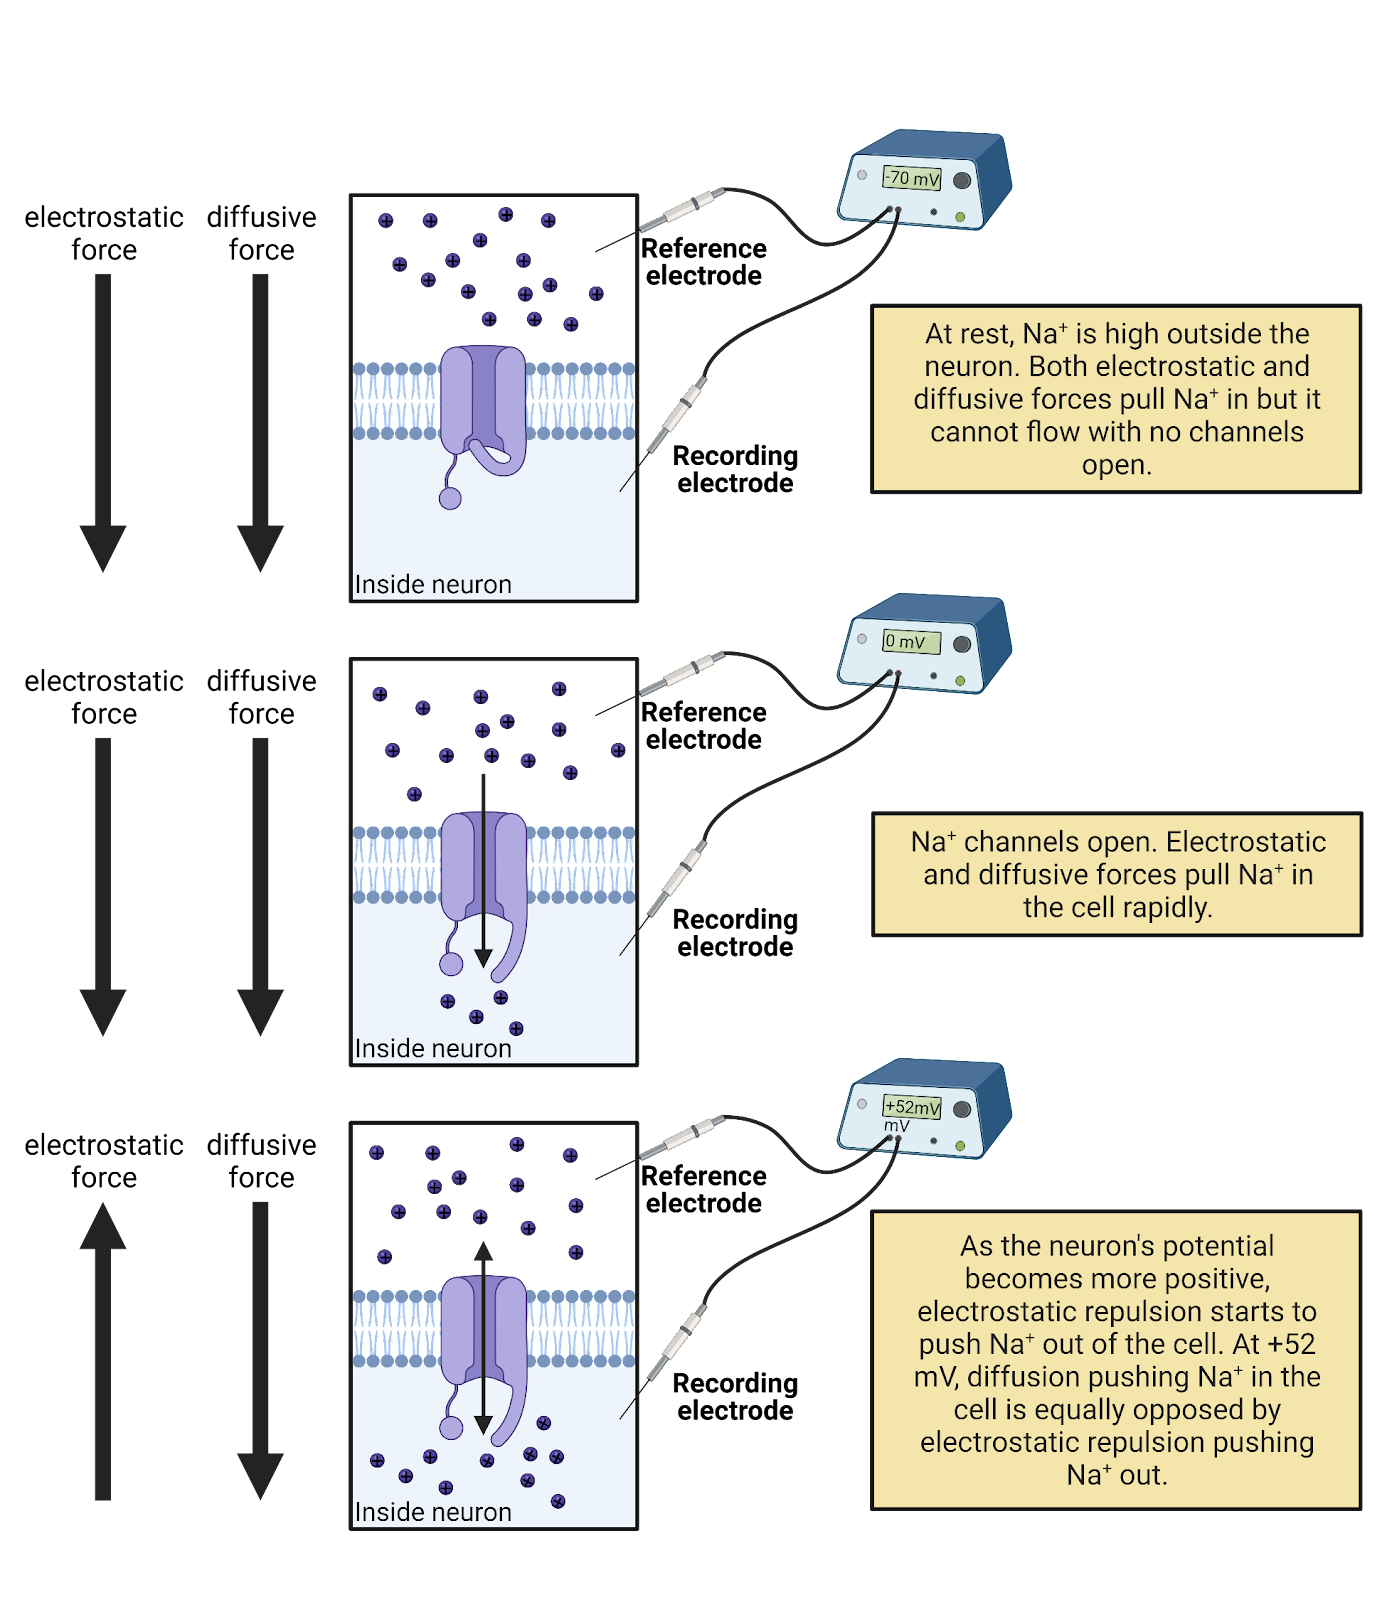
\includegraphics[width=0.8\linewidth]{images/ch02/02_17} 

}

\caption{Ion concentration batteries.}(\#fig:ch02_17)
\end{figure}

Solving the Nernst equation for the other key ions shows that under typical conditions, ECa is 124mV, K+ is -87mV, and Cl is -81mV (Erecińska and Silver, 1994).

What, exactly, do these calculations tell us? That each concentration-gradient battery has the energy needed to charge the neuron to a specific membrane potential. If Ca++ became able to move in/out of a neuron at rest, the concentration-gradient would push Ca++ into the neuron, storing up positive charge inside the neuron until it's membrane potential was pulled up to +124mV (until total charge inside the neuron (Q) divided by capacitance (C) = 124mV). If K+ was able to move, it would move to drag the neuron's membrane potential down to -87mV. Each ion has a distinct concentration and therefore a distinct charge that it would ``like'' to produce in a neuron. Table 2.01 summarizes the concentration-gradient battery for each ion.

From this, we can define an ion's \textbf{driving force }as the distance between a neuron's membrane potential (VM) and the maximum potential that ion's concentration-gradient can produce (Eion):

Driving Forceion = VM - Eion

Even if the complexities of the Nernst equation leave you feeling a bit mystified, here are three key ideas you can hold on to:

\begin{itemize}
\tightlist
\item
  Because of their concentration gradients, both Na+ and Ca++ have a constant pressure to charge neurons up to positive membrane potentials, \emph{if they can} (if there are open Na+ or Ca++ channels). Cl- and K-, on the other hand, have a constant pressure to bring neurons down to negative membrane potentials, \emph{if they can} (if there are open Cl- or K- channels).
\item
  The concentration-gradient batteries in neurons are not very strong compared to the ones that power the electronics around you. A typical cell-phone battery generates an electrical potential of 3.7V. That's about 30x stronger than the Ca++ concentration-gradient battery operating in each of your neurons.
\item
  A neuron's batteries depend on concentration gradients produced by pumps. If concentrations change, the strengths of these batteries are also changed. In addition, it takes energy to keep these batteries charged: Each ion pump in the membrane needs a steady supply of cellular energy (ATP) to work against diffusion. This actually eats up a considerable amount of energy. It is estimated that about 28\% of your brain's large energy budget is devoted to the operation of ion pumps (Lennie, 2003)!
\end{itemize}

\hypertarget{ion-channels-are-selective-but-passive-conductors-some-ion-channels-are-gated.}{%
\subsection{Ion channels are selective but passive conductors; some ion channels are gated.}\label{ion-channels-are-selective-but-passive-conductors-some-ion-channels-are-gated.}}

Look inside a laptop and you'll see a tangle of wires, pathways of high conductance that allow electrical currents to flow. What are the `wires' that carry electrical currents into and out of a neuron? It's not the cell membrane, which has a low conductance. Instead, neurons (and all other cells) express \textbf{ion channels }(Image 2.18). Ion channels are proteins that stick through the membrane. Each has a water-filled \textbf{central pore} through which specific ions can flow with high conductance. Ion channels allow currents of electrolytes to flow into and out of neurons.

\begin{figure}

{\centering 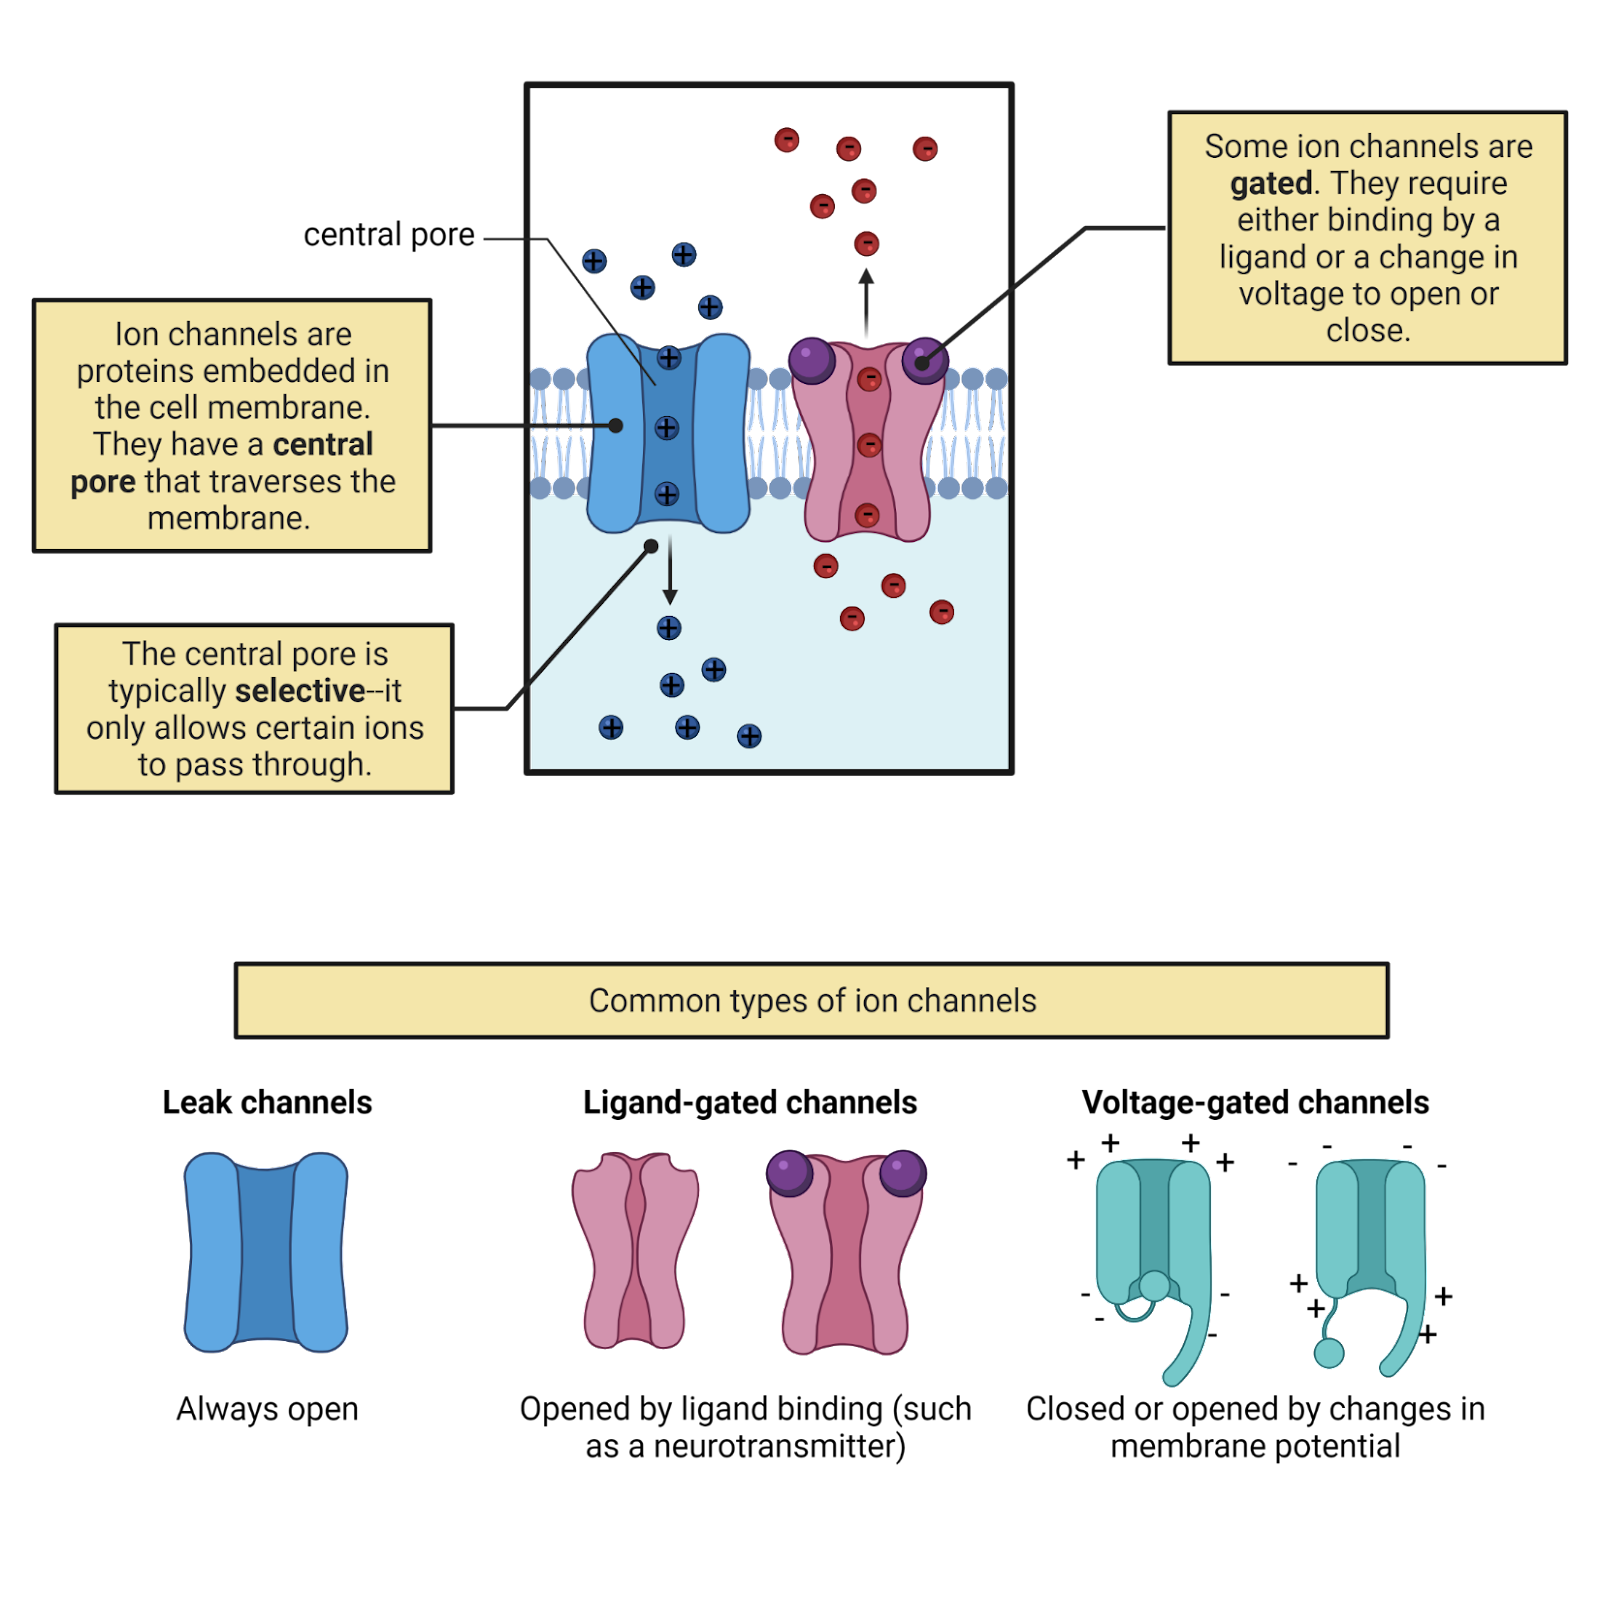
\includegraphics[width=0.8\linewidth]{images/ch02/02_18} 

}

\caption{Ion channels.}(\#fig:ch02_18)
\end{figure}

Unlike pumps, ion channels are \textbf{passive}. Any ion that fits through an ion channel is ``free'' to move through it in either direction. The channel does not add any ``push'' or use energy to direct the flow of ions. Instead, ion movement through channels is determined purely by the pressures operating on that ion (diffusion and electrostatic force). If pressure is pushing a K+ ion into a neuron, it can enter via an open K+ channel, a positive current (because the cell gains a positive charge). If pressure is pushing a K+ ion out of a neuron, it can just as easily \emph{leave} via a K+ channel, a negative current (because the cell loses a positive charge). Table 2.02 gives a detailed comparison between pumps and channels.

\begin{figure}

{\centering 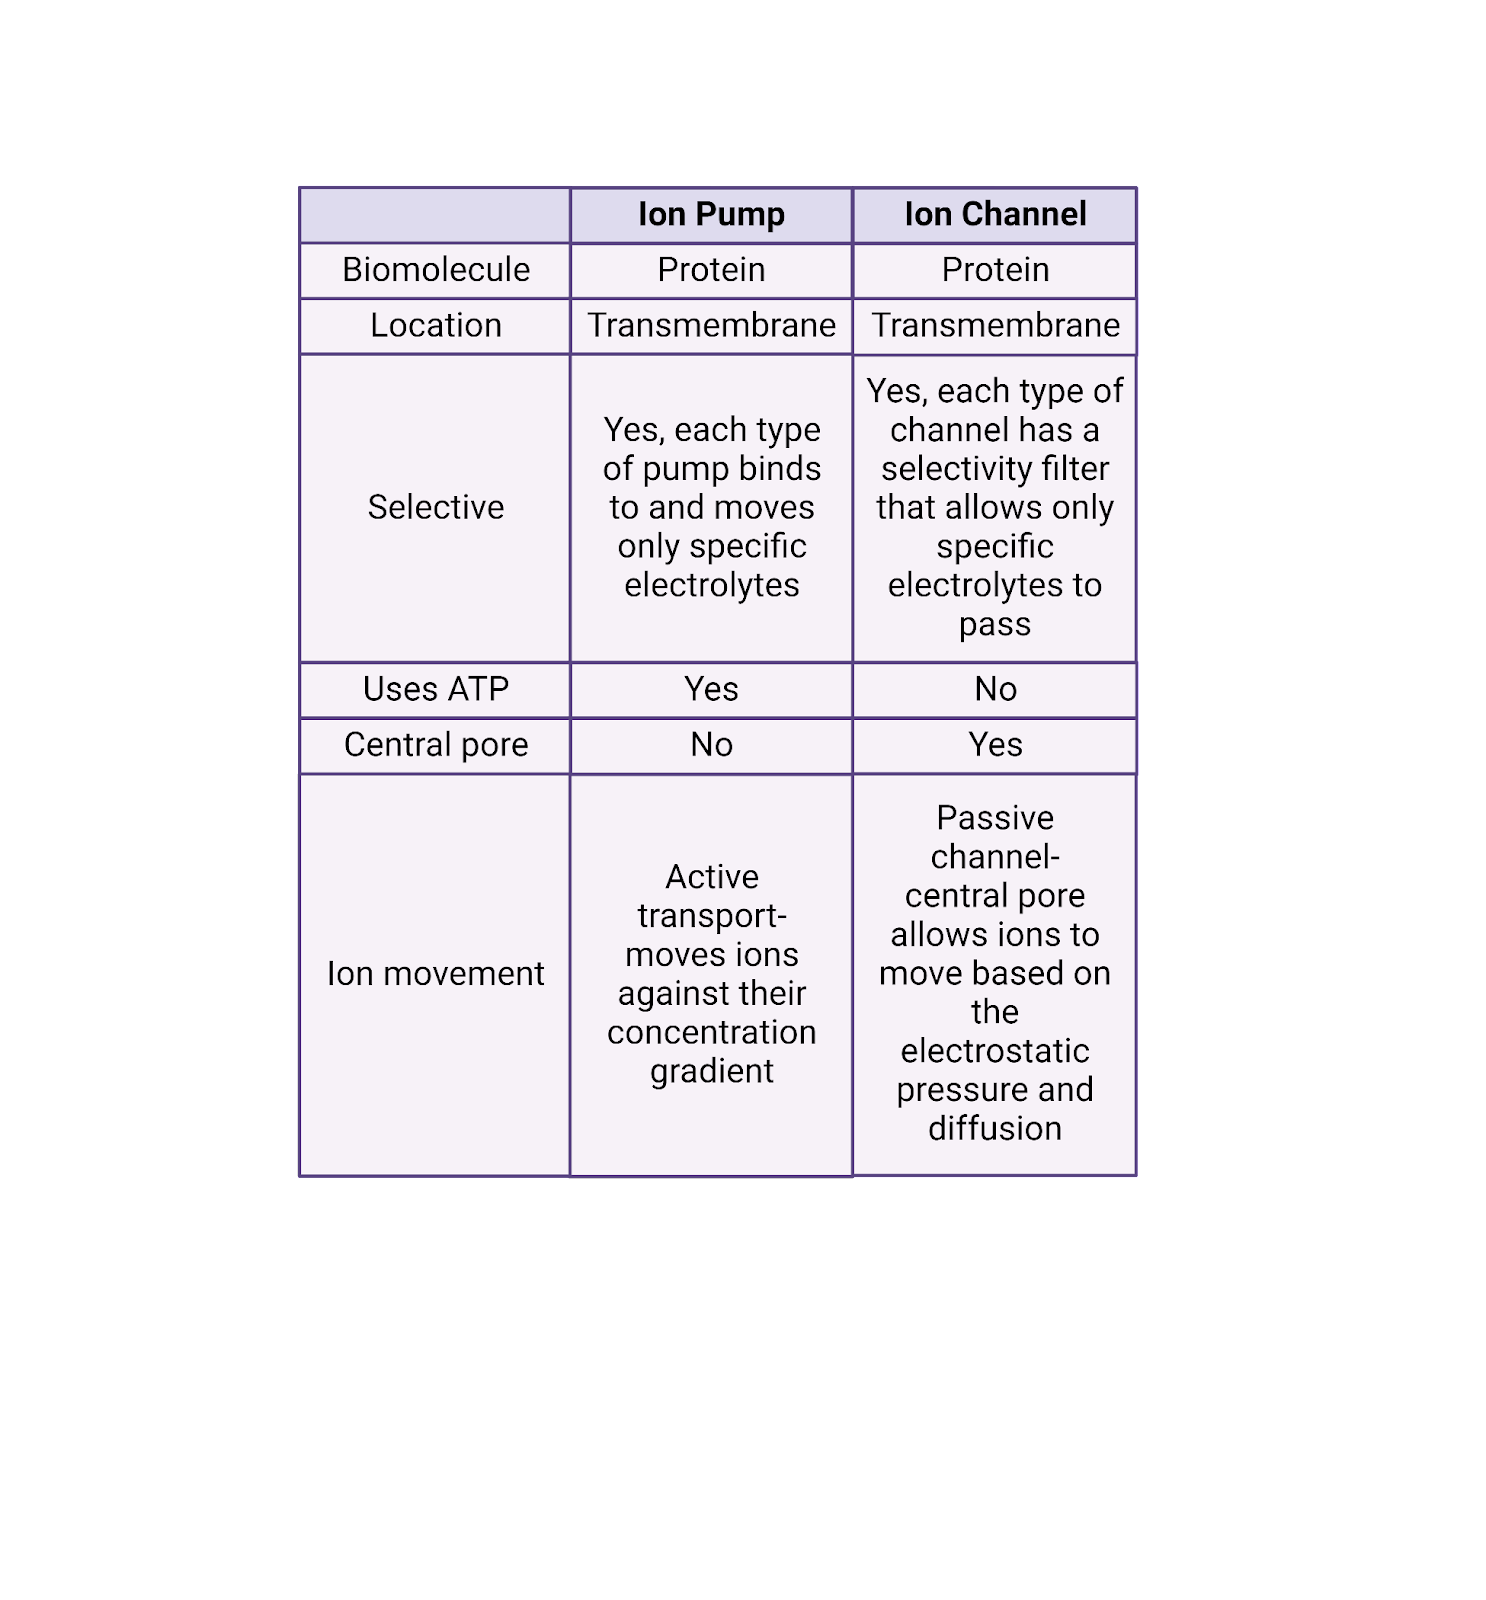
\includegraphics[width=0.8\linewidth]{images/ch02/table_02_01} 

}

\caption{Pumps vs. channels.}(\#fig:table_ch02_02)
\end{figure}

Although ion channels are passive they are nevertheless \textbf{selective}. Some channels are conductive only to Na+; they are called Na+ channels. Other channels are only conductive to K+; they're called K+ channels. As you can probably already guess, there are also Ca++ channels and Cl- channels.

How can an ion channel let one mineral pass but block others? Each ion channel has a \textbf{selectivity filter}, a special region of amino acids that controls which molecules can access the central pore. The selectivity filter ``recognizes'' each mineral based on its charge, size, and sphere of hydration. So, for example, the selectivity filter on a K+ channel works just right with the charge and size of a K+ ion to allow it to easily pass into the central pore of the channel, providing a high conductance for K+ through the channel. Other ions don't pass by the selectivity filter as well, and so have a much lower conductance through a K+ channel (though not always 0).

Some ion channels, called leak channels, are simply a pore with a selectivity filter---they provide a constant selective conductance (Image 2.18). Other ion channels are \textbf{gated}, meaning that they can \emph{switch} from \emph{open} (a conformation with a high conductance) to \emph{closed} (a conformation with a low conductance).

Gated channels don't just open and close will nilly ---they have **sensors\_, \emph{\textbf{specialized sections of their protein structure that determine when they open and when the close. For example, }ligand-gated ion channels} \_\textbf{have sensors that bind to specific neurotransmitters, opening the channel only when the right transmitter is present. }Voltage-gated ion channels** have sensors that detect electrical events a neuron, opening the channel only when the neuron reaches a specific membrane potential. This is just the tip of the iceberg. There is tremendous diversity in the types of gated ion channels neurons can express. Chapters 6, 7, 8, and 9 will introduce some of the fascinating gated ion channels that enable sensory neurons to respond to events in the outside world.

An open ion channel provides a \textbf{conductance} for that ion, a pathway that allows the flow of current if that ion is under pressure. This means the number of ion channels matters. For example, the more K+ ion channels a neuron expresses, the larger the total K+ conductance possible for K+ in that neuron (the more possible routes for K+ current when these channels are open). This actually takes us back to Ohm's law, which expresses this mathematically:

Iion = Gion * (VM -- Eion)

This means the current produced for an ion is the product of its conductance (how many ion channels are open) and the driving force for that ion (the distance between the neuron's current membrane potential and the maximum potential the ion's concentration gradient can produce).

There is tremendous diversity in ion channels. Your DNA has genes that code for several hundred different types of ion channel. For this chapter, we'll focus in on 3 key families that are critical for neural signaling: 1) leak K+ and Na+ channels that maintain the resting potential, 2) ligand-gated channels that produce EPSPs and IPSPs, and 3) voltage gated Na+ and K+ channels that produce the action potential.

\hypertarget{topic-summary-2}{%
\subsection{Topic summary}\label{topic-summary-2}}

This section was a crash course in the physics of neural signaling. If you made it through, you've seen that pumps are protein machines that use energy to build up concentration gradients of 4 key electrolytes, pushing K+ into neurons and Na+, Cl-, and Ca++ out of neurons. The concentration gradients produced by pumps function as chemical batteries: they provide an entropic ``push'' for K+ to and Cl- to charge the neuron towards negative potentials and Na+ and Ca++ to charge the neuron towards positive neurons. The cell membrane holds back this push of diffusion, but ion channels provide gated and selective conducatances for ionic currents. Ohm's law describes the movement of ions to produce the electrical signals in neurons: Iion = Gion * (VM -- Eion). This tells us that the movement of each type of ion is determined by two factors: 1) the number of open channels for that ion (Gion; the ion's total conductance), and 2) the driving force produced by that ion's concentration-gradient battery (VM -- Eion). Each ionic current flowing through a channel moves charge in or out of a neuron and therefore modifies Vm, its membrane potential: dV/dt = I/C. The physics of neural electricity can be a bit daunting, but it provides a foundation from which we have built a detailed and powerful understanding of neural signaling.

\textbf{Key Terms}

Voltage-sensitive fluorescent protein

Propagation

Ion pumps

Ion channels

Electrolytes

Charge, measured in Coulombs

Electrostatic force

Ion

Current, measured in Amperes (amps), symbol is \emph{Q}

Conductance, measured in Seimens, symbol is \emph{G}

Insulator

Electrical potential, measured in Volts, symbol is \emph{V}

Ohm's law

Membrane potential, symbol is \_VM \_usually graphed as a function of time

Electrode, recording electrode, reference electrode

Neurophysiology

Solute

Diffusion

Concentration gradient

Sphere of hydration

Capacitance, measured in Farads, symbol is C

Concentration gradient

Battery

Nernst equation

Driving force

Ion channel -- have a central pore, passive, selective, sometimes with a sensor and gate

Selectivity filter

Ligand-gated ion channel

Voltage-gated ion channel

\textbf{References and works cited}

\begin{itemize}
\item
  Erecińska M, Silver IA (1994) Ions and energy in mammalian brain. Prog Neurobiol 43:37--71.
\item
  Kralj JM, Douglass AD, Hochbaum DR, Maclaurin D, Cohen AE (2012) Optical recording of action potentials in mammalian neurons using a microbial rhodopsin. Nat Methods 9:90--95 Available at: \url{http://www.nature.com/articles/nmeth.1782}.
\item
  Lennie P (2003) The Cost of Cortical Computation. Curr Biol 13:493--497 Available at: \url{https://linkinghub.elsevier.com/retrieve/pii/S0960982203001350}.
\end{itemize}

\hypertarget{neurophysiology-mechanisms}{%
\section{Mechanisms of neural signaling}\label{neurophysiology-mechanisms}}

\textbf{Learning objectives}

By the end of this section, students will be able to:

\begin{itemize}
\tightlist
\item
  Objective 1: Explain how the resting potential is generated and defended primarily by leak K+ channels, which allow the K+ concentration-gradient battery to generate K+ currents that constantly pull membrane potential towards EK, a negative charge.\\
\item
  Objective 2: Understand the role of ligand-gated ion channels in producing EPSPs and IPSPs, the small, transient, and local changes in membrane potential that represent the receipt of transmitter from partner neurons.\\
\item
  Objective 3: Describe how the action potential is generated by the sequential opening of voltage-gated inactivating Na+ channels (allowing Na+ in to produce the rising phase) and voltage-gated K+ channels (which allows K+ to depart, accelerating the falling phase and producing the undershoot).
\end{itemize}

Before we took our deep dive into bioelectricity, we marveled at a video that used voltage-sensitive dyes to let us ``see'' action potentials spreading rapidly through a neuron. We're now ready to unravel this fascinating signal, to learn about the incredible interplay of pumps, channels, and ions that allow each of your 86 billion neurons to generate the constant barrage of electrical signals that make you who you are. We'll start by exploring the resting potential, then we'll examine how this `rest' is perturbed by EPSPs and IPSPs imposed by synaptic partners. Finally, we'll dissect the action potential and its rapid spread throughout the axon to produce transmitter release. Before you read on, it can help to get a bird's eye view from Table 2.03, which breaks down the properties of the resting potential, post-synaptic potentials, and the action potential.

\begin{figure}

{\centering 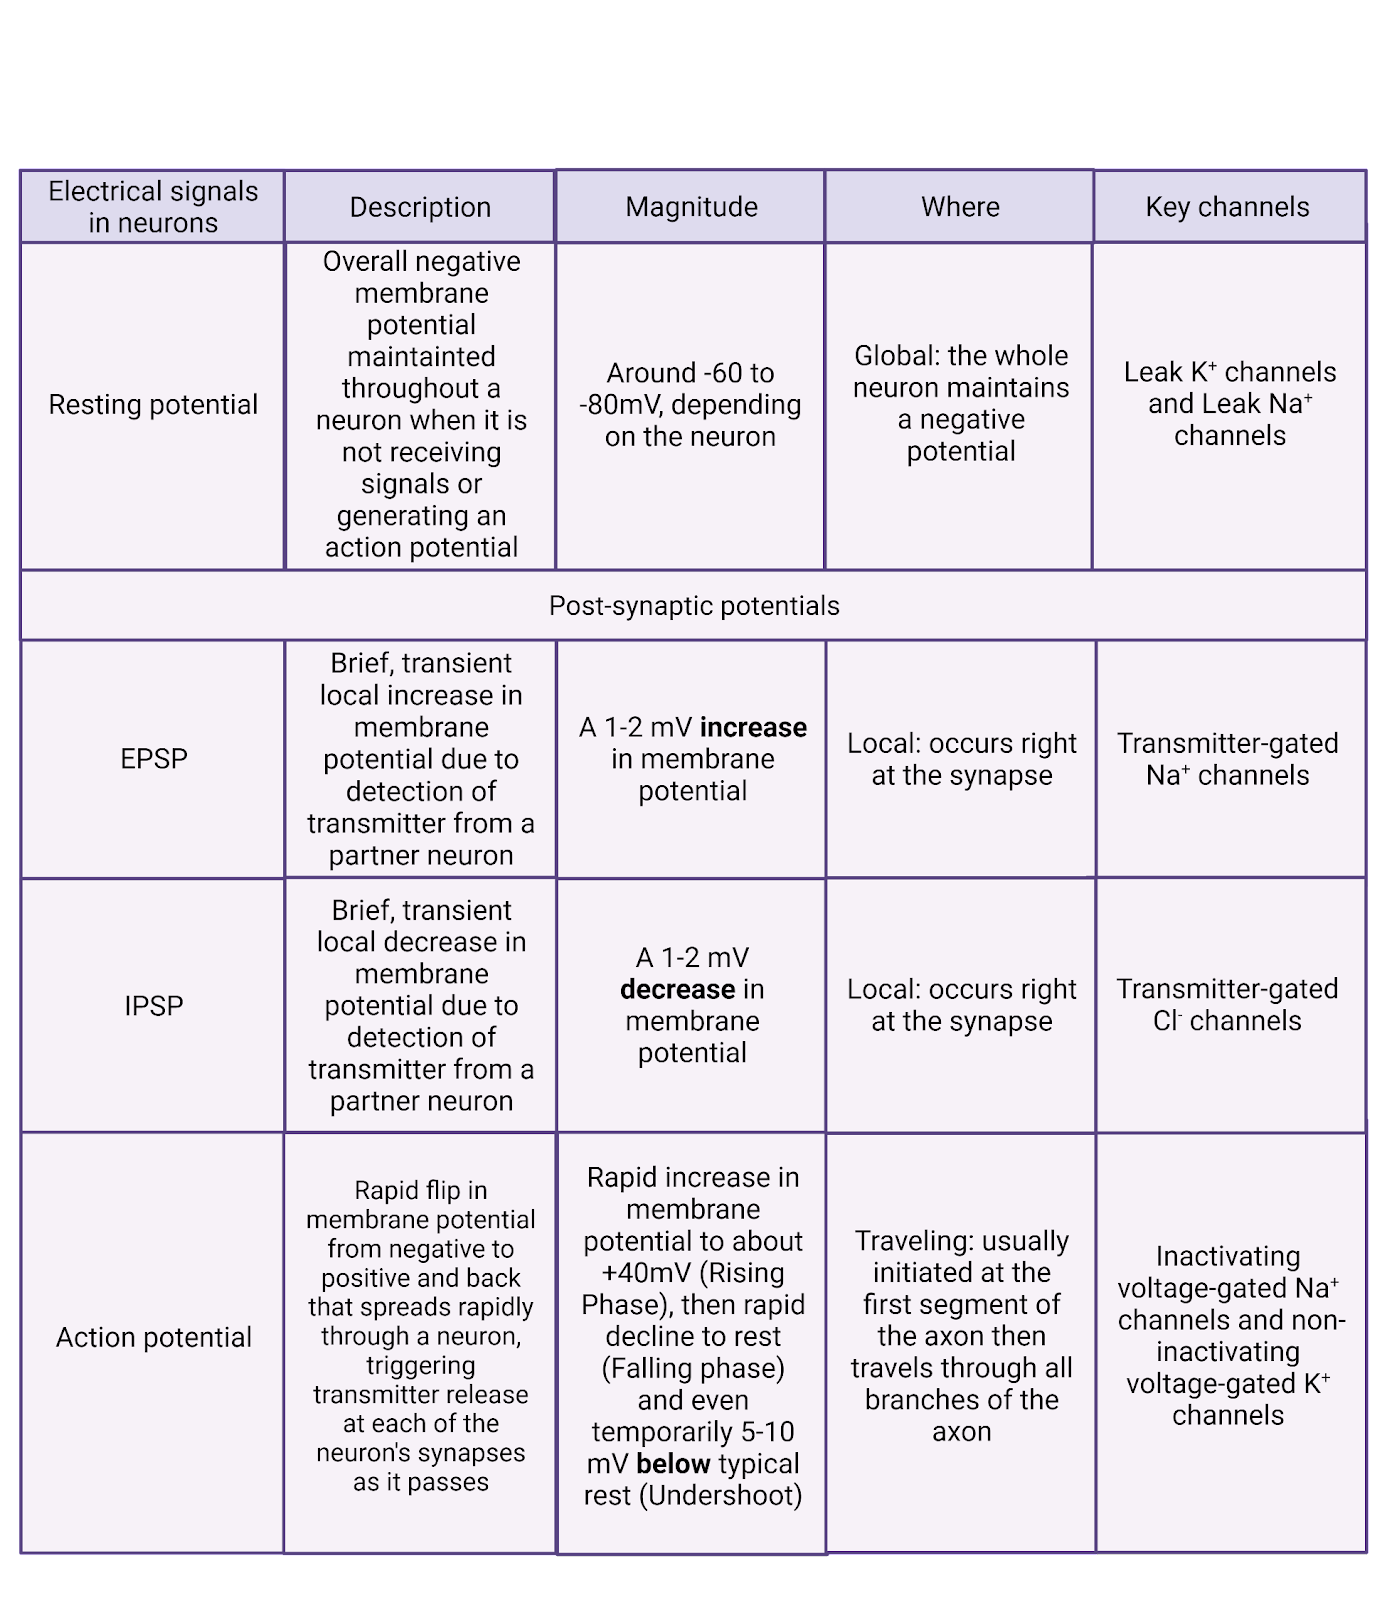
\includegraphics[width=0.8\linewidth]{images/ch02/table_02_03} 

}

\caption{Types of electrical signal.}(\#fig:table_ch02_03)
\end{figure}

\hypertarget{the-resting-potential-is-produced-by-leak-channels-and-concentration-gradients.}{%
\subsection{The resting potential is produced by leak channels and concentration gradients.}\label{the-resting-potential-is-produced-by-leak-channels-and-concentration-gradients.}}

The **resting potential\_ \_**is an overall negative charge maintained by a neuron, typically around -65mV (though the exact value varies from neuron to neuron and can change). Neurons are sometimes said to \emph{`defend'} their resting potential, meaning that after any stimulation they have a strong tendency to return quickly to rest. Neurons are not alone in having a resting potential---most of the cells in your body also maintain an overall weak negative charge.

The resting membrane potential is due to 2 families of ``leak'' ion channels: \textbf{leak K+ channels} and \textbf{leak Na+ channels}. Leak channels are channels that are always open, having no gating (Image 2.19).

\begin{figure}

{\centering 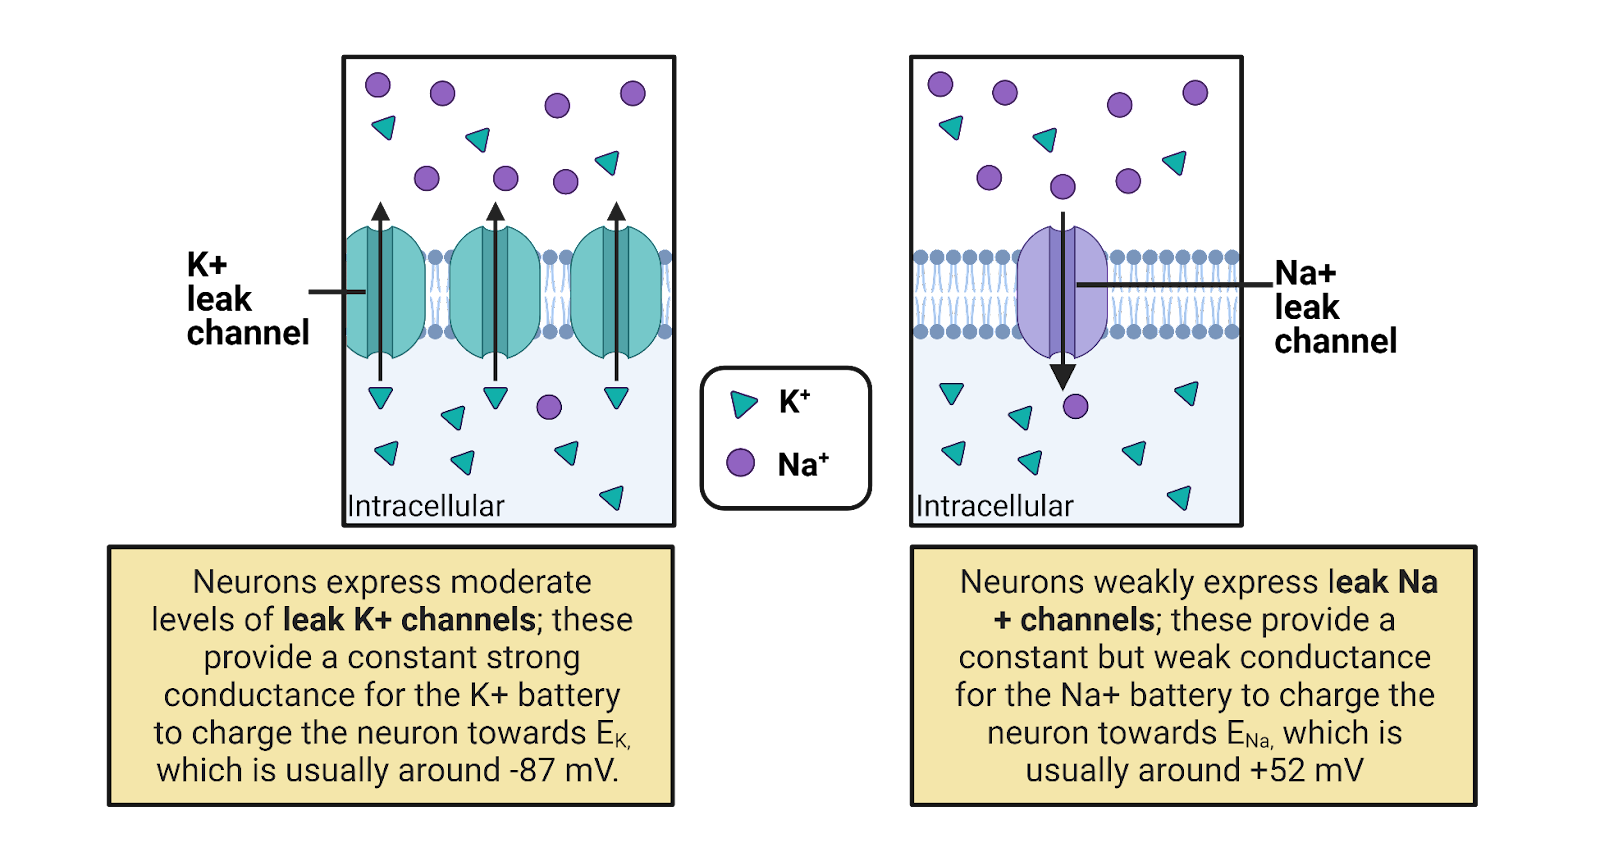
\includegraphics[width=0.8\linewidth]{images/ch02/02_19} 

}

\caption{Leak channels.}(\#fig:ch02_19)
\end{figure}

Leak K+ channels are moderately expressed in neurons, providing a constant but modest conductance for K+. The leak K+ channels allow the concentration-gradient battery for K+ to constantly work to charge the membrane towards EK, a very negative potential (-87 mV in a typical neuron). The combination of the leak K+ channels and the concentration gradient battery for K+ act like a tractor-beam that constantly pulls a neuron's membrane potential towards a strongly negative potential. Any time a neuron becomes excited, reaching a more positive potential, the driving force on K+ is increased (that's the distance between the neuron's charge and EK, see Table 2.01). This increase in pressure pushes K+ out through the leak channels, and the resulting departure of K+ pulls the neuron's membrane potential back down towards rest (Image 2.20). This is what we observe as the ``defense'' of the resting membrane potential---there is always a conductance that allows the K+ battery to charge the neuron towards EK., a negative membrane potential.

\begin{figure}

{\centering 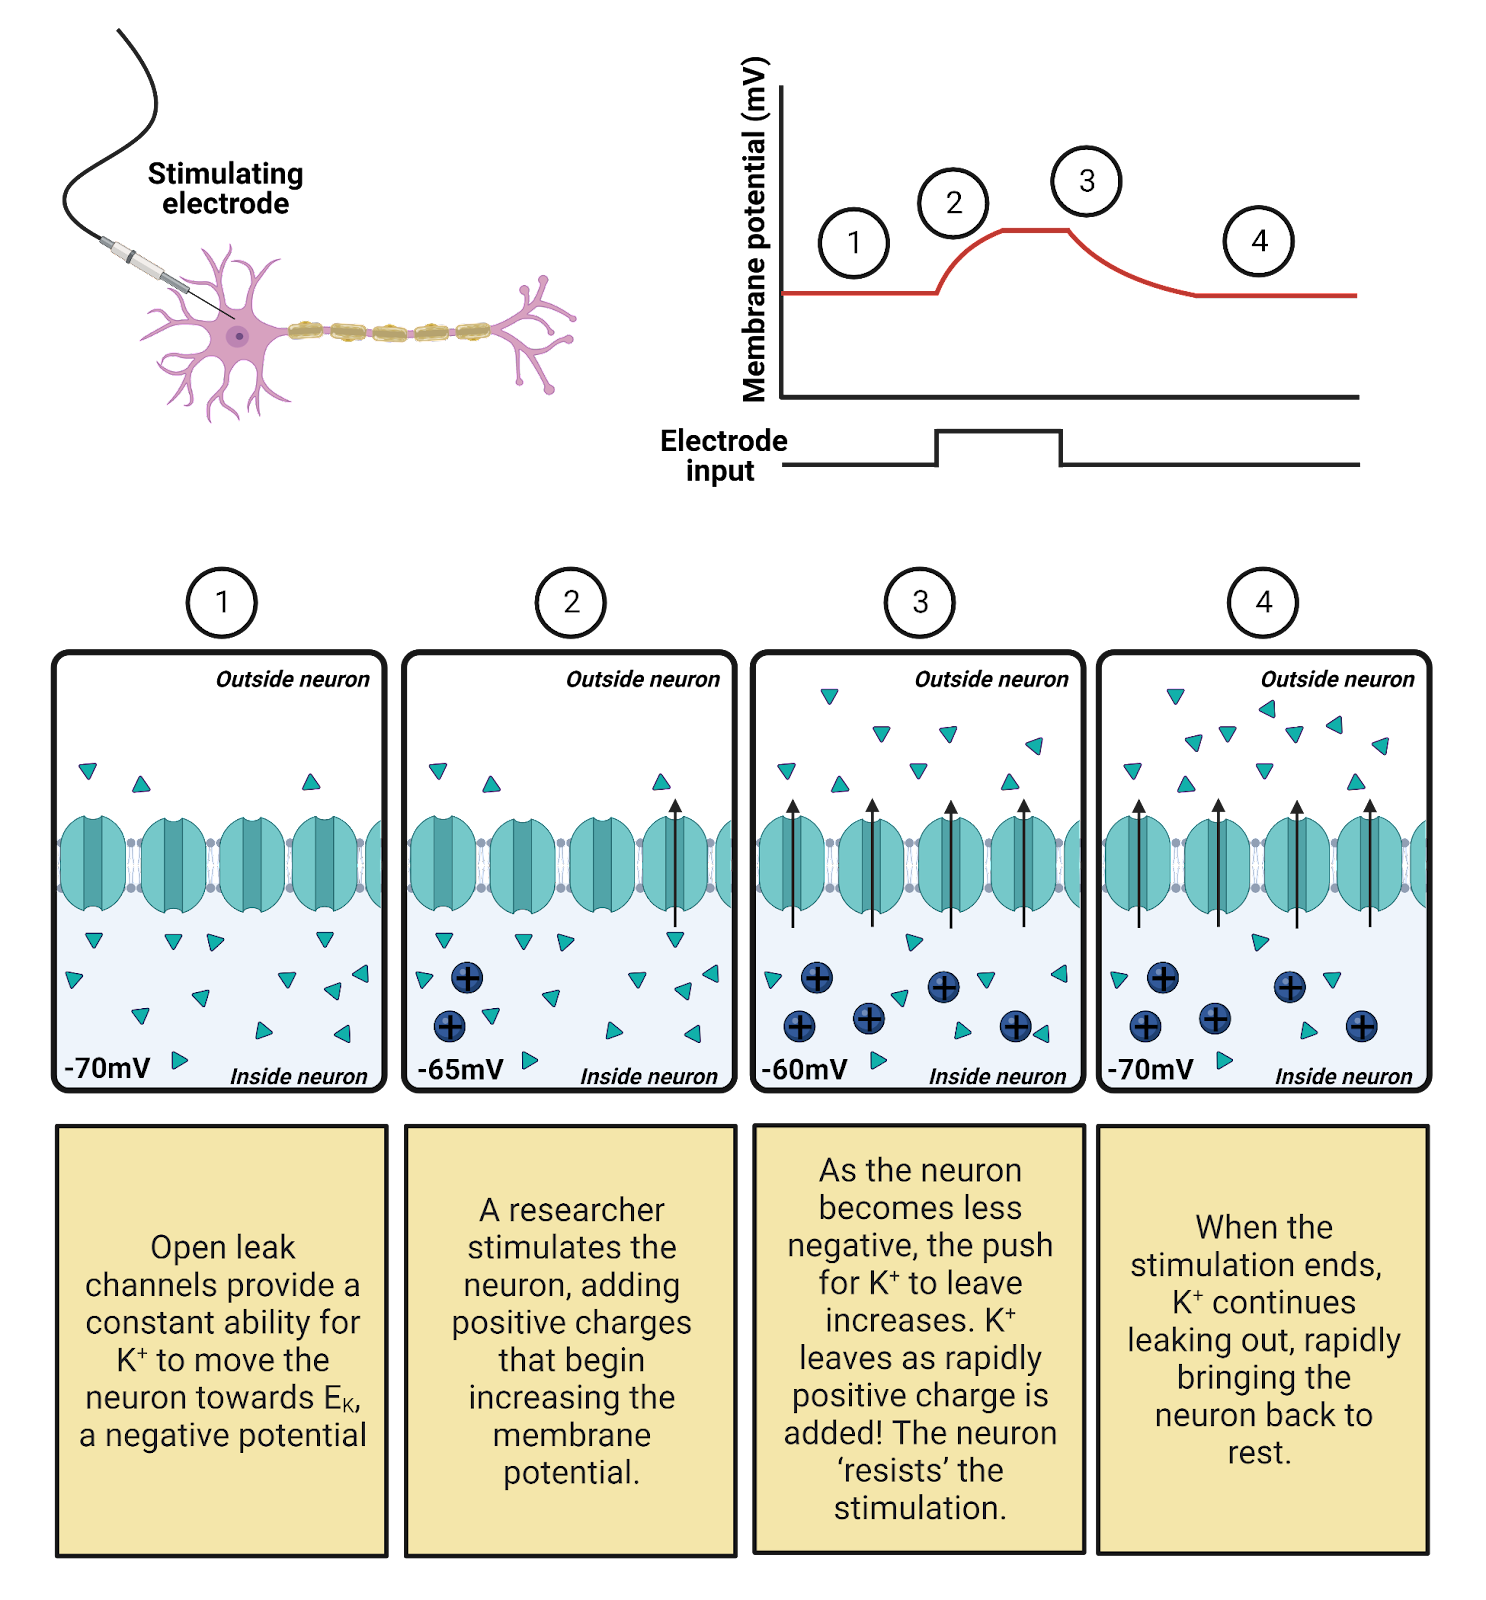
\includegraphics[width=0.8\linewidth]{images/ch02/02_20} 

}

\caption{Leak channels defend the resting potential.}(\#fig:ch02_20)
\end{figure}

Although the K+ battery can deliver a charge of around -87 mv, the resting membrane potential is a good bit higher, around -65mV. Why? Because neurons also weakly express leak Na+ channels, with about 1 leak Na+ channel for every \textasciitilde7 leak K+ channels. This means that there is also a constant, but weak, conductance for Na+ that allows Na+ to enter, trying (in vain) to pull the neuron towards a positive membrane potential. In other words, there is a constant ``tug of war'' between the K+ and Na+ batteries. Because there are more leak K+ channels, the K+ battery mostly wins this tug of war, holding the resting membrane potential close to EK, the maximal charge the K+ battery can deliver. Still, the expression of leak Na+ channels pulls the resting membrane potential a bit higher.

There is a cost to this tug of war between K+ and Na+. It means that even at rest there is a constant, though small, departure of K+ and a constant, though small, influx of Na+. Ion pumps must work constantly to undo this slow leak of current, otherwise the concentration-gradient batteries would eventually become depleted.

\hypertarget{post-synaptic-potentials-are-produced-by-ligand-gated-channels.}{%
\subsection{Post-synaptic potentials are produced by ligand-gated channels.}\label{post-synaptic-potentials-are-produced-by-ligand-gated-channels.}}

EPSPs and IPSPs are small, local, temporary changes in the membrane potential that are produced when neurotransmitter is received from synaptic partners. Each post-synaptic potential is an electrical translation of a chemical message that helps determine if an action potential will be generated.

EPSPs and IPSPs are produced by \textbf{ligand-gated ion channels }(Image 2.21). These are transmembrane proteins with a central pore. Each has an external \emph{binding site} that recognizes a specific neurotransmitter. When a molecule of neurotransmitter fits into the binding site the channel is pulled open; when no transmitter is present, the channel stays closed. The post-synaptic side of each synapse is studded with hundreds of ligand-gated ion channels, so each burst of transmitter release from the pre-synaptic neuron produces a temporary but substantial opening of channels on the post-synaptic membrane, translating the chemical transmitter signal into a sharp change in conductance that allows current to flow.

\begin{figure}

{\centering 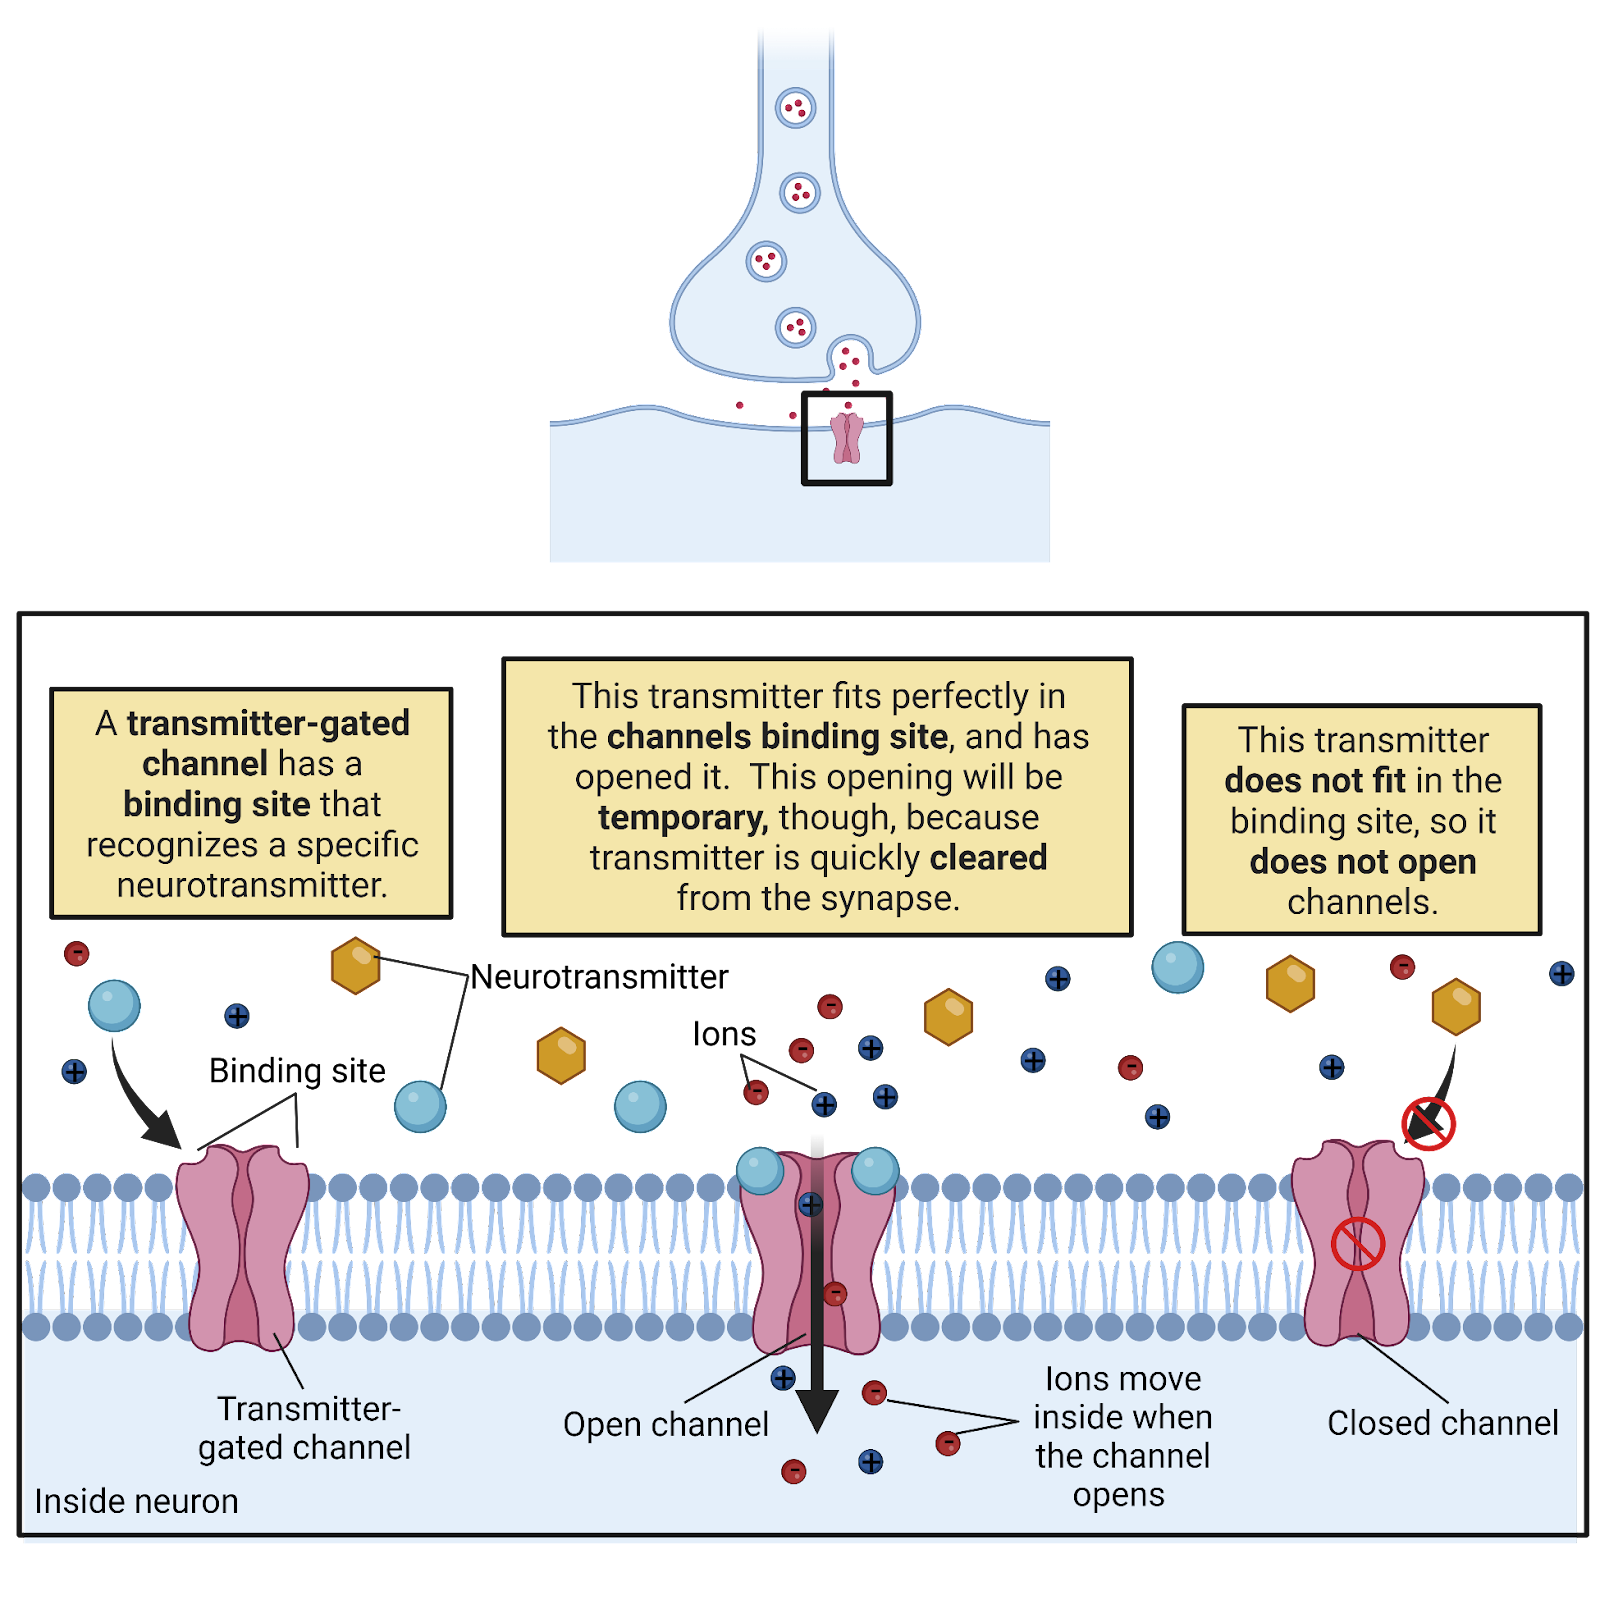
\includegraphics[width=0.8\linewidth]{images/ch02/02_21} 

}

\caption{Transmitter-gated channels.}(\#fig:ch02_21)
\end{figure}

There is tremendous diversity in ligand-gated ion channels, with the human genome containing genes encoding several hundred ligand-gated ion channels (Viscardi et al., 2021). Part of this diversity is due to differences in binding sites, with different receptors specialized for detecting different neurotransmitters. You have glutamate channels that have a binding site that recognizes the neurotransmitter glutamate, acetylcholine channels that recognize acetylcholine, and much more. The chapter on Neurochemistry will discuss the different classes of neurotransmitters and their receptors in more detail. Another part of the diversity of ligand-gated ion channels is their selectivity: some are selective for Cl-, others for Ca++, others for Na+ or K+.

What happens when a ligand-gated ion channel opens? That depends on its selectivity. If the channel is selective for Cl-, the channel produces IPSPs (Image 2.22). That is because in a neuron at rest there is a driving force for Cl- to enter the neuron (ECl is typically around -81mV, a bit more negative than rest, see Table 2.01). The higher outside concentration of Cl- enables diffusion to push Cl- through the open ligand-gated channels, producing a negative current that makes the neuron's membrane potential more negative and therefore further away from the threshold for generating an action potential. If the channel is selective for Na+ or Ca++, the channel produces EPSPs (Image 2.22). That is because both Na+ and Ca++ carry a positive charge and are more concentrated outside the neuron than in, giving them a very large driving force to enter a neuron at rest. Therefore, an increase in conductance for these ions provides an opportunity for diffusion to produce a \emph{positive} current that would make the neuron's membrane potential more positive and closer to threshold.

\begin{figure}

{\centering 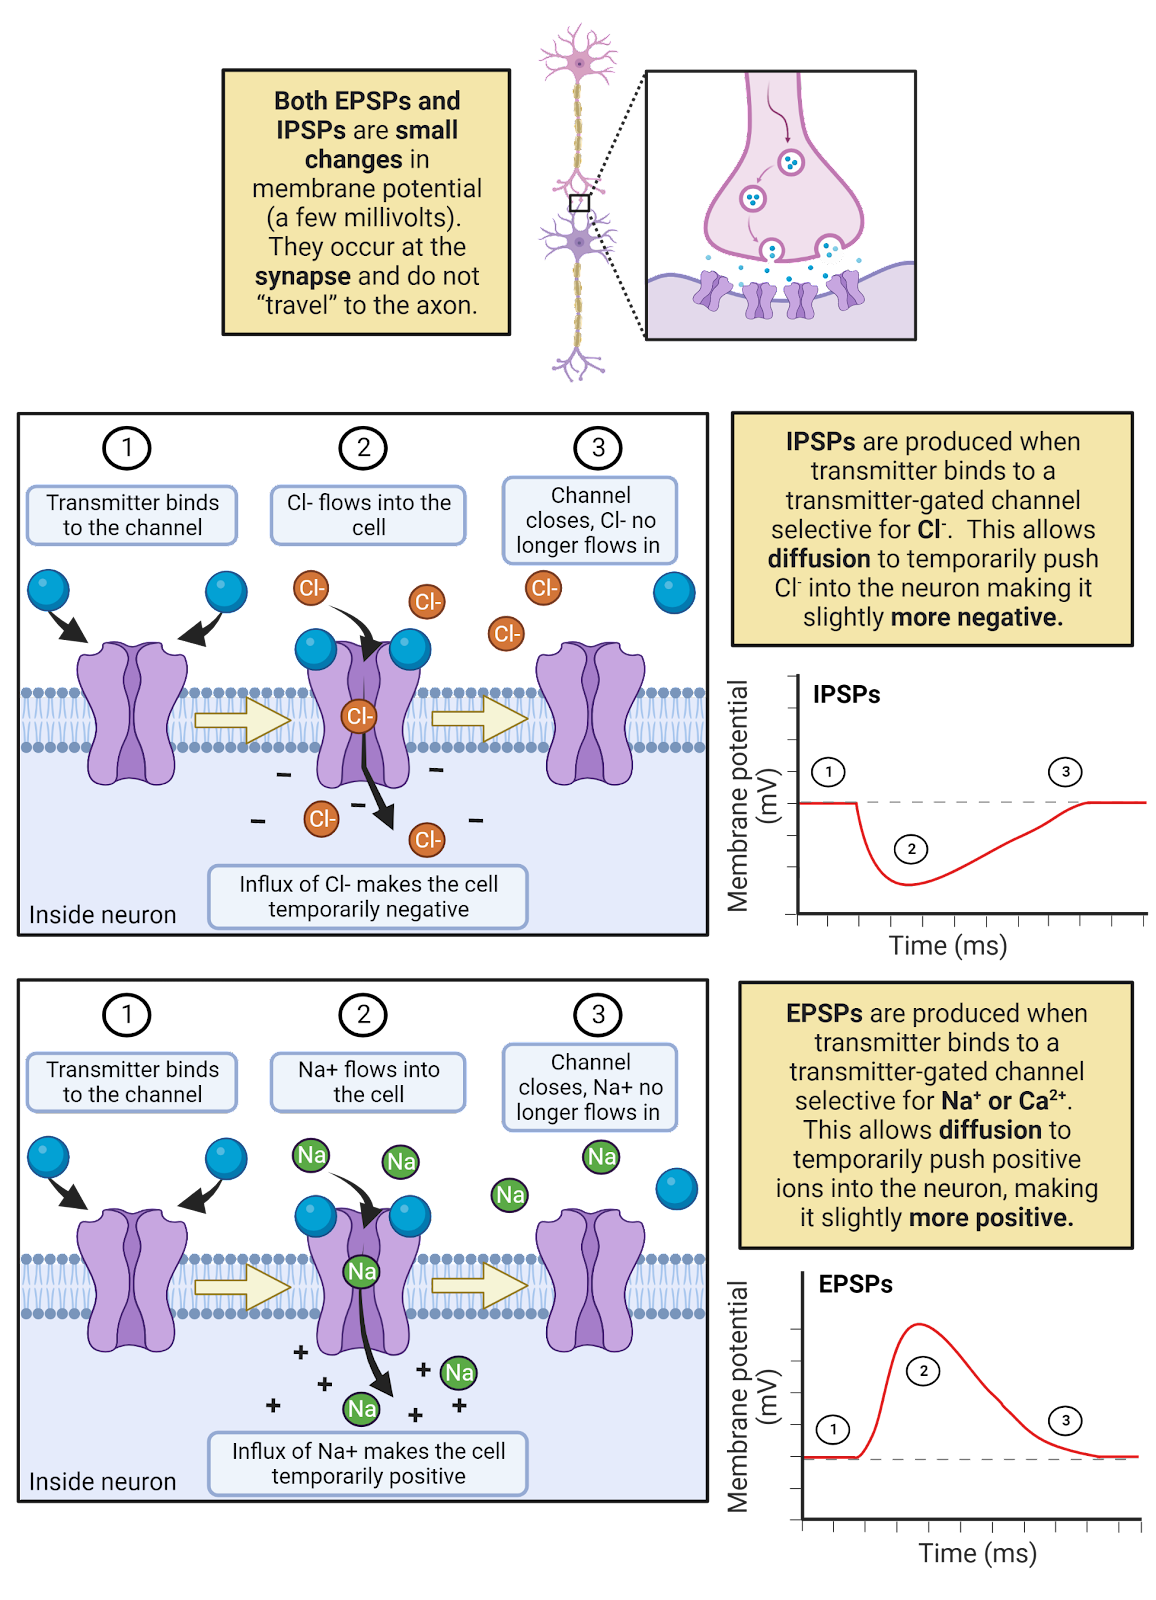
\includegraphics[width=0.8\linewidth]{images/ch02/02_22} 

}

\caption{EPSPs and IPSPs.}(\#fig:ch02_22)
\end{figure}

EPSPs and IPSPS are \emph{transient}, meaning short-lived. First, as discussed earlier, neurotransmitter released into a synapse is very quickly broken down and/or recycled. As the neurotransmitter is cleared from the synapse, the ligand-gated channels close. In addition, the leak K+ channels quickly allow K+ to push the membrane potential back towards rest. For example, during an EPSP, Na+ enters a neuron, a positive current. This increases the membrane potential, but it also increases the driving force for K+ to \emph{leave} the neuron through the open K+ leak channels, a negative current that quickly pushes the neuron right back down to its resting potential.

EPSPs and IPSPs are also \emph{local}. Ligand-gated channels allow ions to flow right at the synaptic membrane, temporarily changing the membrane potential only in a small area around the post-synaptic membrane. Although EPSPs can trigger an action potential which spreads through the axon, neither EPSPs nor IPSPs themselves propagate throughout a neuron.

EPSPs and IPSPs are often relatively small relative to a neuron's threshold. For example, in a human cortical neuron, a single EPSPs is estimated to increase the membrane potential at the soma by only 0.3 mV, whereas the threshold for generating an action potential usually requires about a 30mV increase in potential (Eyal et al., 2018). This means it would typically take about a hundred EPSPs occurring around the same time to trigger an action potential in a resting cortical neuron. Given that a typical neuron has thousands of synaptic partners, receiving 100 excitatory messages at about the same time is a fairly common occurrence--but not so common that a neuron is relentlessly activated.

\begin{itemize}
\tightlist
\item
  EPSPs and IPSPs are integrated both temporally and spatially, meaning inputs are summed over a window of time (temporally) and from all over the neuron (spatially) to influence the production of action potentials (Image 2.23).
\item
  EPSPs and IPSPs are also slow compared to the action potential. It takes time for transmitter to be expelled and to diffuse across the synaptic cleft. This ``synaptic delay'' means it takes about 5ms from a neuron firing an action potential to the peak of the EPSPs or IPSPs in that neuron's post-synaptic partners.
\item
  Transmitters can also produce modulation by binding to receptors that activate intracellular processes. This is covered in more detail in the chapter on Neurochemistry
\item
  It is difficult to comprehend the magnitude of interconnectedness among neurons in the human CNS. While there is an average of 7,000 synaptic contacts per cortical neuron, many neurons are even more interconnected, with a typical pyramidal neuron having about 30,000 synaptic inputs (Eyal et al., 2018) and some modulatory neurons releasing transmitter to millions of other neurons.
\end{itemize}

\begin{figure}

{\centering 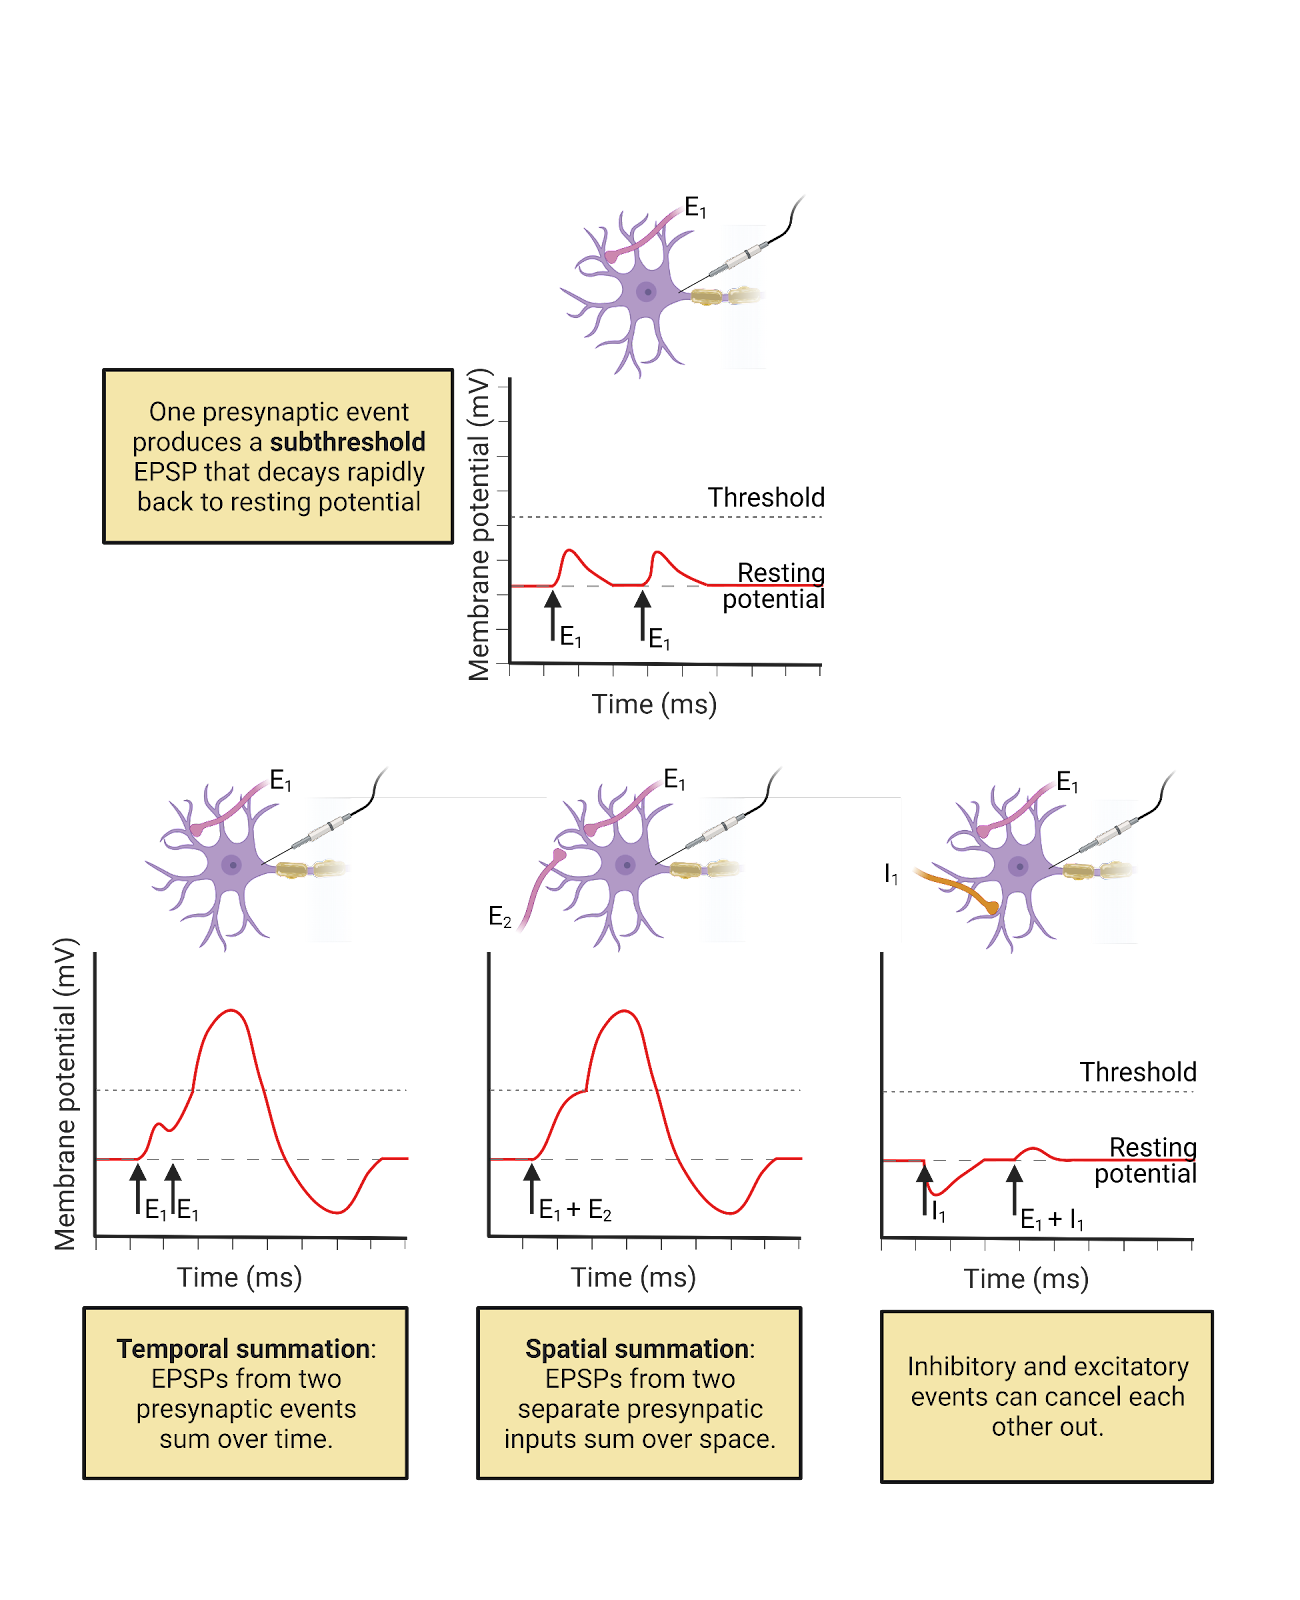
\includegraphics[width=0.8\linewidth]{images/ch02/02_23} 

}

\caption{Temporal and spatial summation.}(\#fig:ch02_23)
\end{figure}

\hypertarget{the-action-potential-is-produced-by-sequential-opening-of-voltage-gated-na-and-k-channels.}{%
\subsection{The action potential is produced by sequential opening of voltage-gated Na+ and K+ channels.}\label{the-action-potential-is-produced-by-sequential-opening-of-voltage-gated-na-and-k-channels.}}

The \textbf{action potential} is a rapid up-and-down of electrical potential that spreads through a neuron to trigger transmitter release. Action potentials usually initiate in the cell body or right at the point where an axon branches off from the cell body, a point called the \textbf{initial segment}. During an action potential, the membrane potential at the initial segment goes from the negative resting potential up to a \emph{positive} potential and then back again. Then this same rise and fall of potential occurs a bit further down the axon, then even further down, and so on. As the action potential \textbf{propagates}down the axon, it triggers transmitter release at each pre-synaptic membrane it passes.

At each point in the axonal membrane the rise and fall of electrical potential is rapid and dramatic (Image 2.24). During the \textbf{rising phase}, the neuron's membrane potential goes from the resting potential of about -65 mv all the way up to a positive potential of around 40mV (though this varies from neuron to neuron). In a typical cortical neuron this upward climb in potential takes only about 0.5ms. This is followed immediately by the \textbf{falling phase}, when the neuron's membrane potential descends just as quickly, falling back down to a negative potential and becoming even \emph{more} negative than during the typical resting potential, often reaching about -85mV. The descent ``below'' rest is called the \textbf{undershoot}, and it takes a typical cortical neuron about 4-5 ms to gradually return to the typical resting potential. This means that every time a neuron fires an action potential, it temporarily moves further away from threshold than when at rest. This helps avoid excessive activity.

\begin{figure}

{\centering 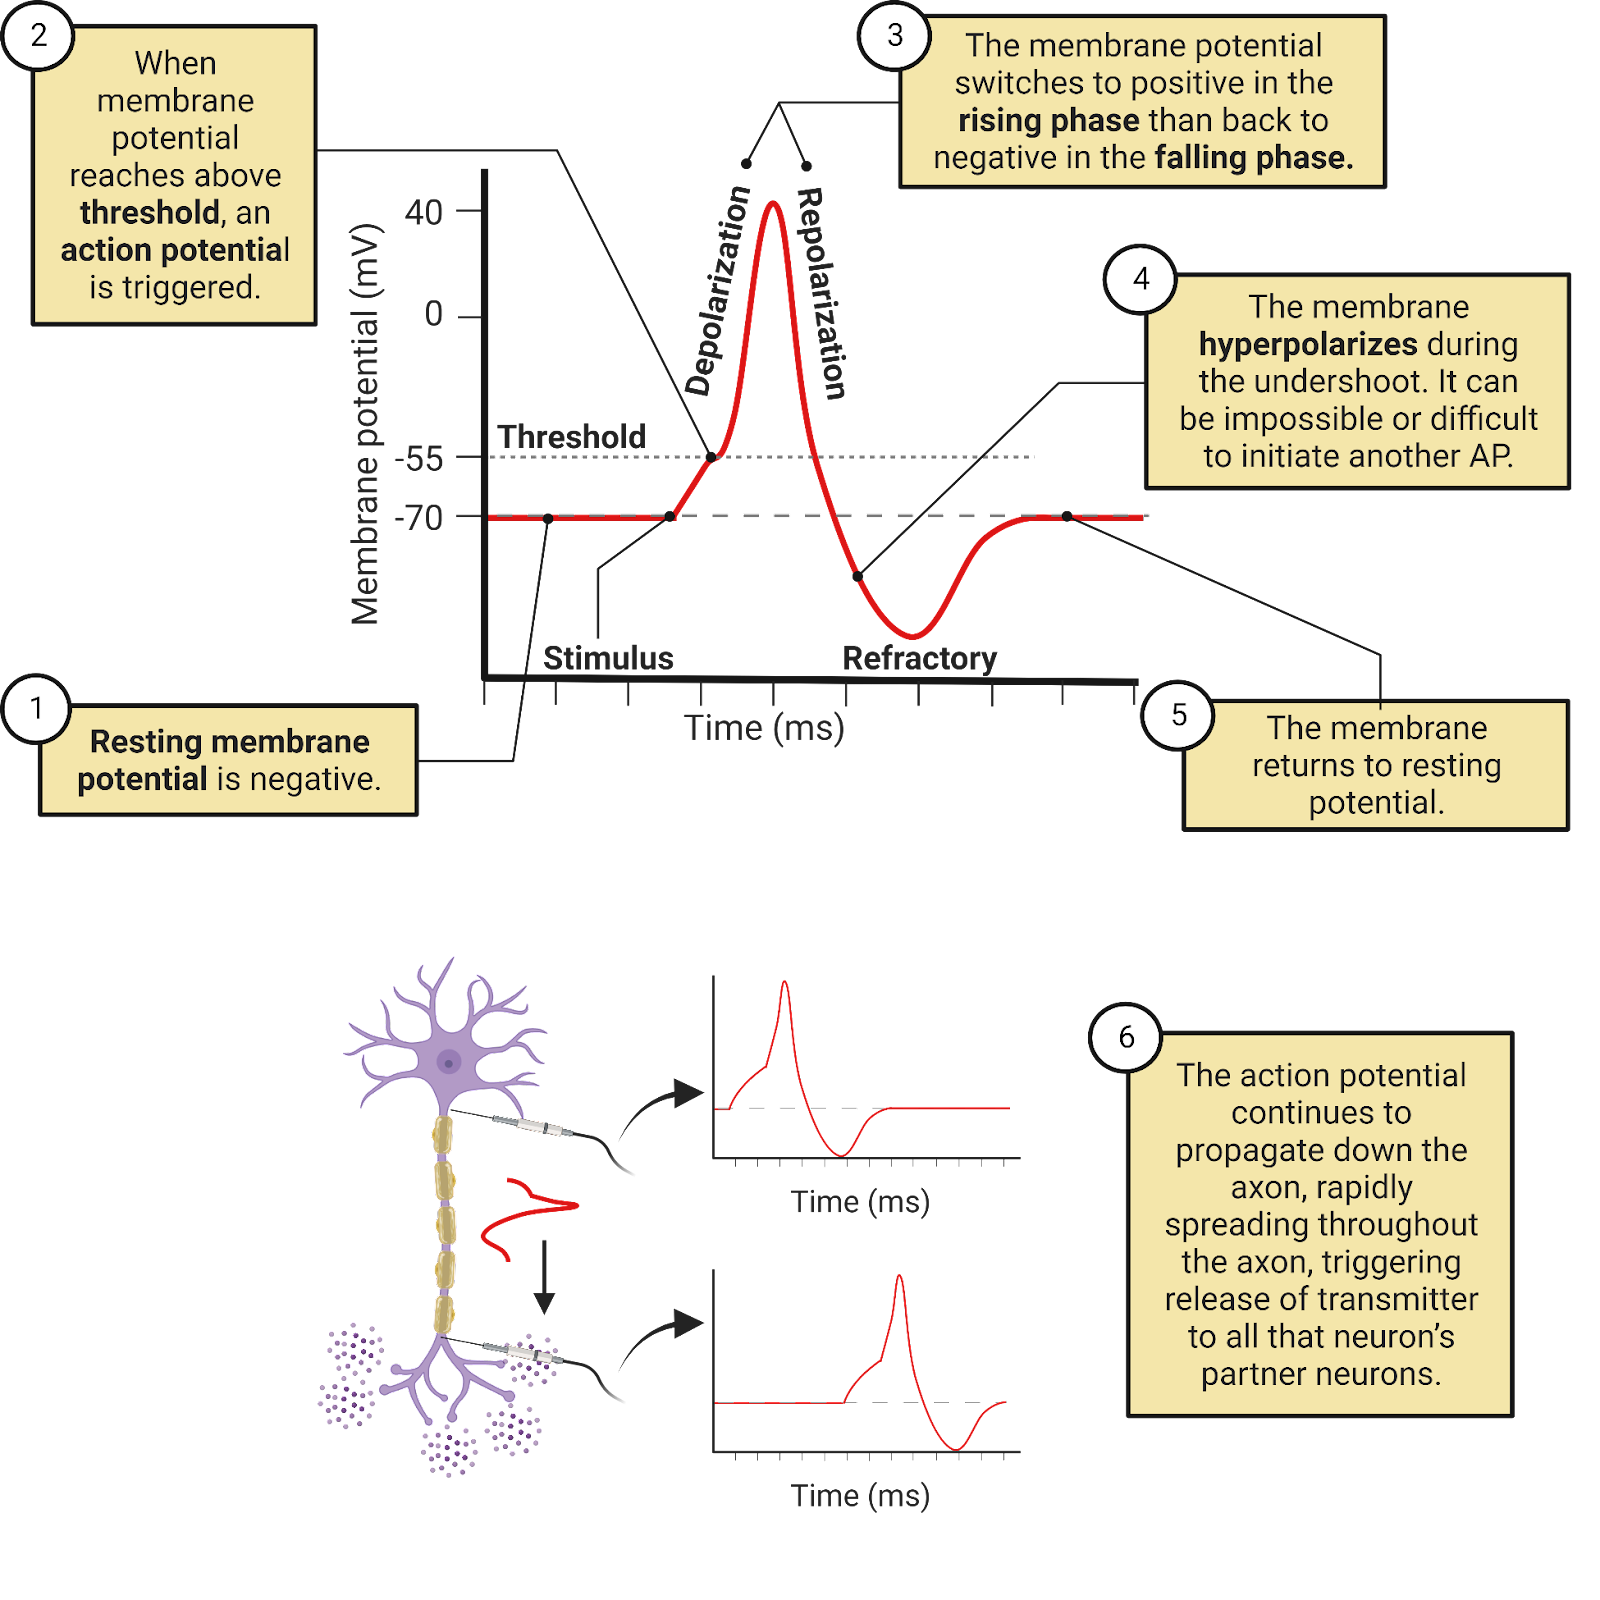
\includegraphics[width=0.8\linewidth]{images/ch02/02_24} 

}

\caption{Phases of the action potential.}(\#fig:ch02_24)
\end{figure}

The action potential is due to the operation of two specialized ion channels that are relatively unique to neurons: inactivating voltage-gated Na+ channels and non-inactivating voltage-gated K+ channels (Image 2.25).

Inactivating voltage-gated Na+ ion channels are highly expressed in neurons, and are often targeted specifically to the initial-segment and axon. Scientists classify these channels as \textbf{voltage-gated} because they have a sensor that holds them closed when a neuron is near its negative resting potential, but that then pulls them open when a neuron's membrane potential increases. A better name, though, would be \emph{excitation gated}, because it is EPSPs from partner neurons that can make a neuron's membrane potential positive enough to open these channels. This gating of the voltage-gated Na+ channels is what we observe as the \textbf{threshold }for an action potential. The exact membrane potential sufficient to open the voltage-gated Na+ channels varies from neuron to neuron and can change, but in a typical cortical neuron, the voltage-gated Na+ channels open at around -35mv. As mentioned earlier, this threshold is high enough that in a typical human cortical neuron it is estimated that it requires EPSPs from over a hundred partner neurons to reach threshold and trigger an action potential.

\begin{figure}

{\centering 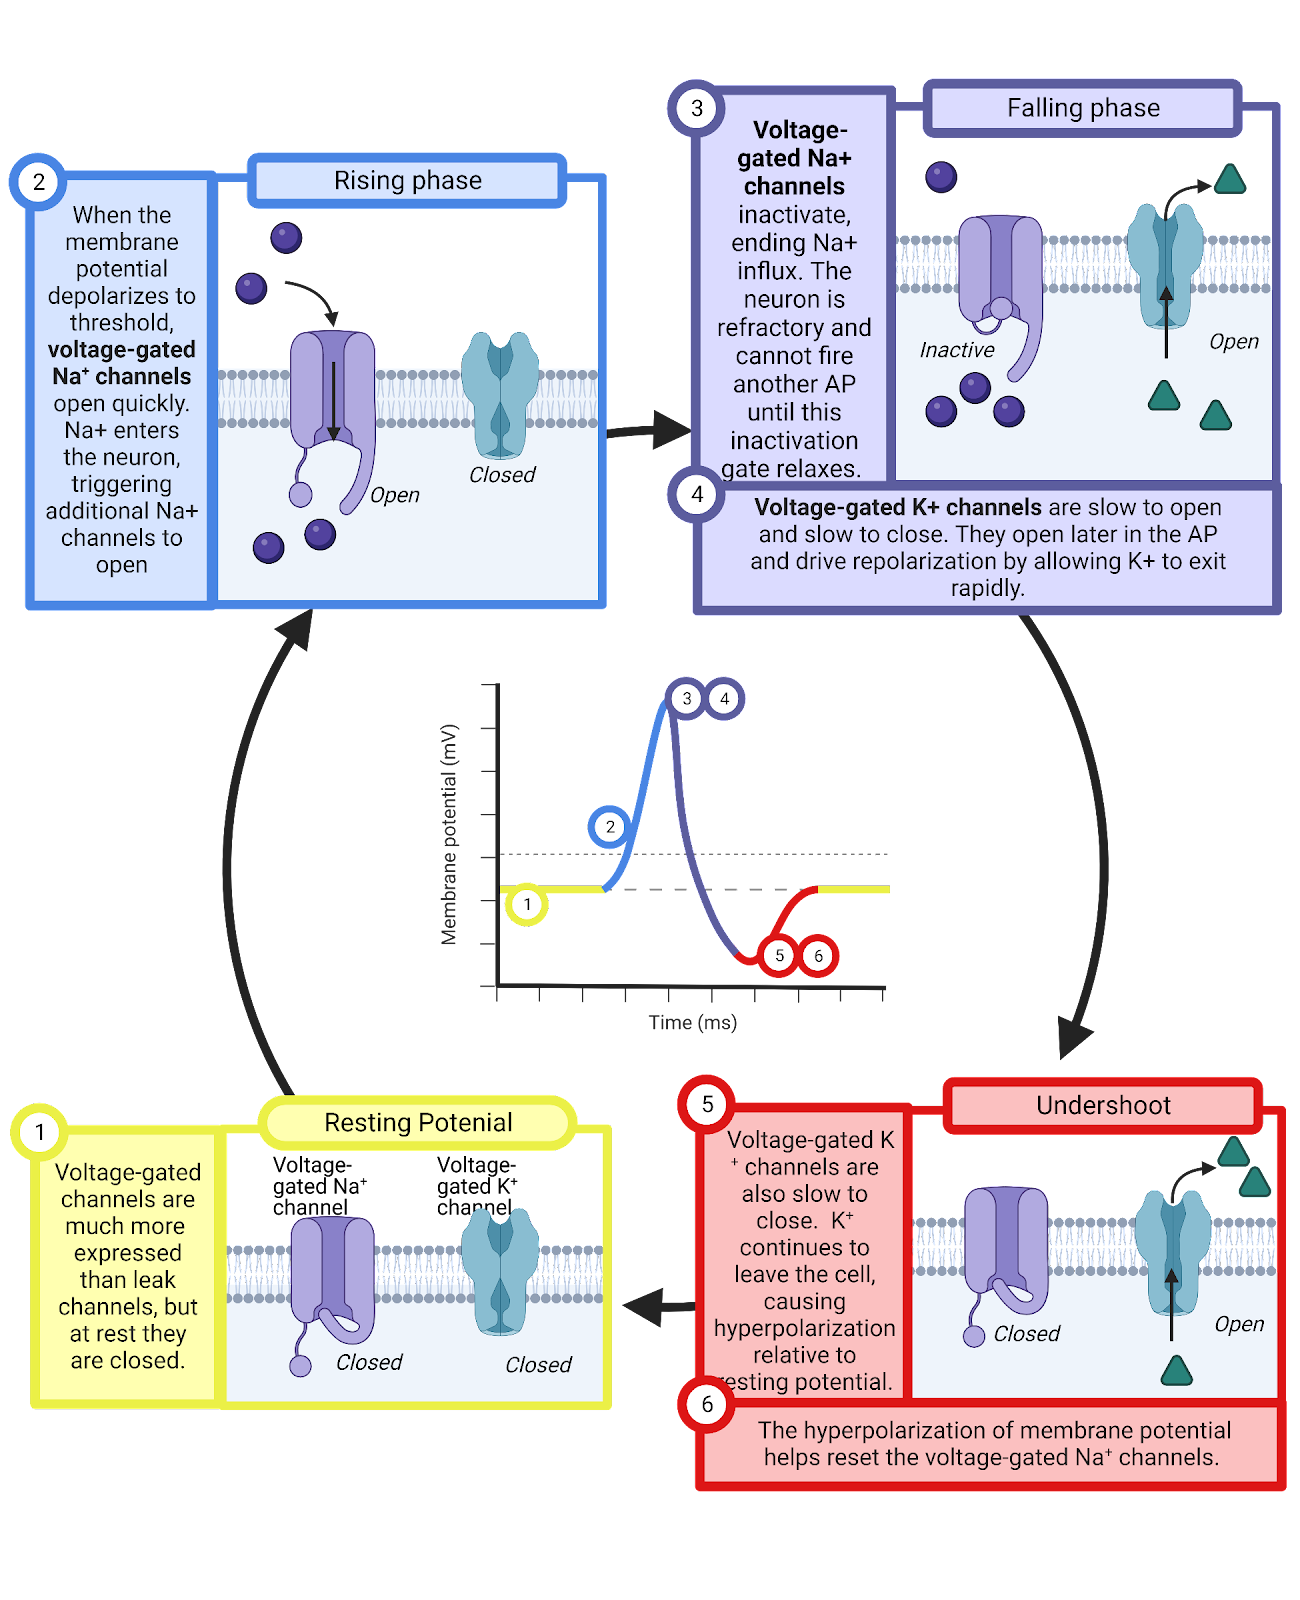
\includegraphics[width=0.8\linewidth]{images/ch02/02_25} 

}

\caption{Action potential generation.}(\#fig:ch02_25)
\end{figure}

The opening of the inactivating voltage-gated Na+ channels produces a sharp increase in conductance for Na+. This gives the Na+ battery a sudden and huge advantage in its ``tug of war'' with the K+ battery: there are now many pathways available for diffusion to push Na+ into a neuron along with a huge driving force for Na+ to enter the neuron (ENa is far from the resting potential, indicating an unmatched pressure of diffusion for Na+ to enter the neuron, see Table 2.01). The result is rapid influx of Na+ so extreme that it quickly pulls the neuron's membrane potential all the way up to a positive membrane potential. This is whatis what we observe as the rising phase of an action potential.

If an EPSP can increase the membrane potential enough to open \emph{one} voltage-gated Na+ channel, then a chain reaction can be triggered. The first voltage-gated Na+ channel to open allows Na+ to enter, causing an increase in membrane potential---the very thing that can trigger the opening of \emph{more} voltage-gated Na+ channels! This \textbf{positive-feedback} loop, where each Na+ channel that opens can help trigger additional openings causes the action potential to \emph{propagate} down the axons, triggering transmitter release at all that neuron's pre-synaptic terminals along the way (Image 2.26).

\begin{figure}

{\centering 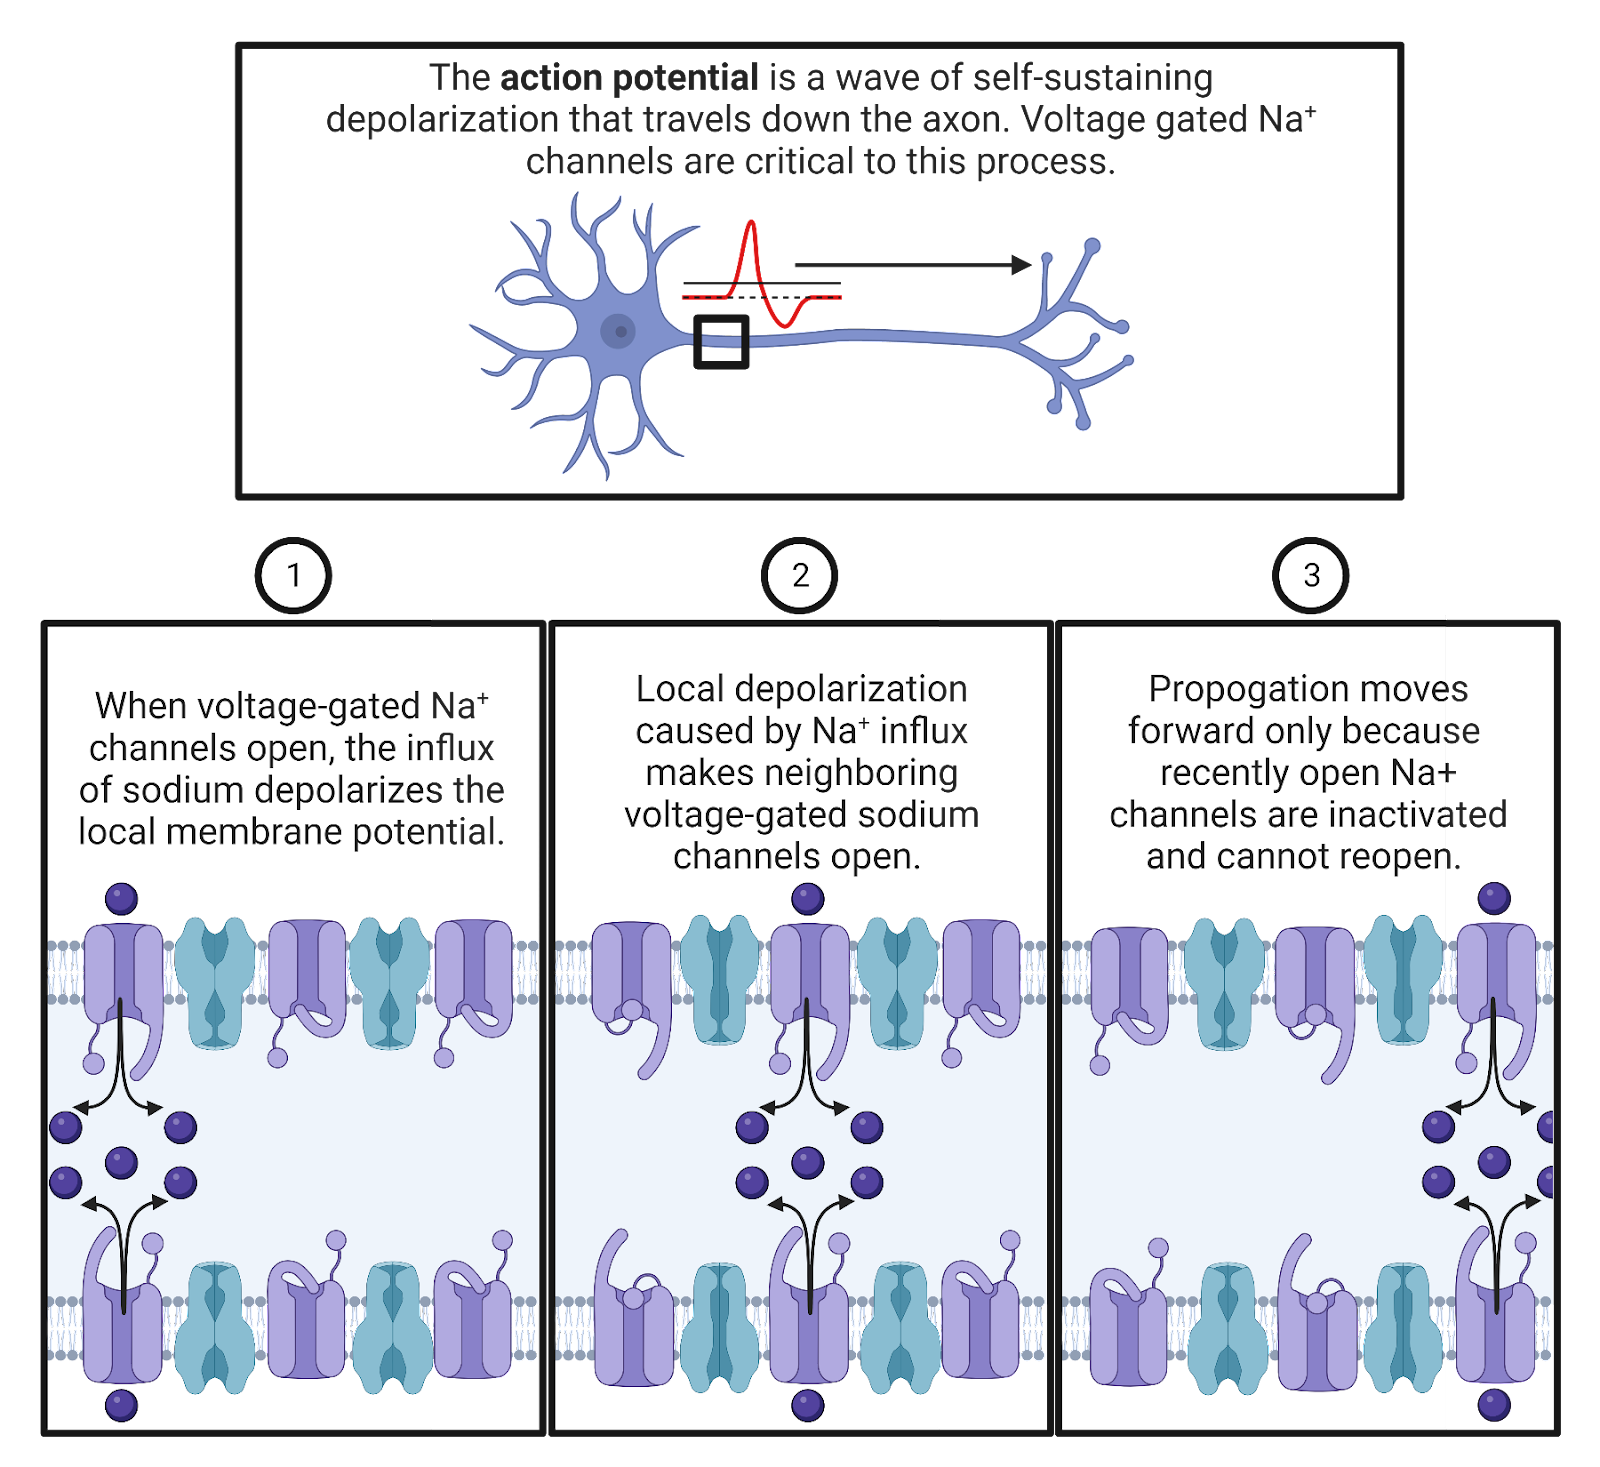
\includegraphics[width=0.8\linewidth]{images/ch02/02_26} 

}

\caption{Action potential propagation.}(\#fig:ch02_26)
\end{figure}

Although action potentials spread, they are very brief: the rising phase is followed very quickly by a plunge back down to a negative potential. One factor limiting the rising phase is the \emph{inactivation} of the voltage-gated Na+ channels. Each channel has a ``tail'' of positively charged amino acids on the intracellular side of the membrane. When these channels open and drive a neuron to a positive potential, the tail is repelled, and this repulsion actually pushes it into the channel, clogging it! Even though the voltage-sensor is still pulling the channel open (because the neuron has a positive membrane potential), the inactivating tails temporarily eliminates the Na+ conductance through these channels.

The clogging of the inactivating voltage-gated Na+ channels is reversible. When a neuron returns to a negative resting potential, that negative charge attracts the positive charges in the inactivating tails, pulling them out of the Na+ channels so that they can work again. This amazing system helps prevent excessive activity in the nervous system: once a neuron generates an action potential, it cannot generate another until it returns to rest and the majority of its channels are unclogged. We observe this as a brief \textbf{refractory period }that occurs immediately after each action potential. Together with the undershoot, the refractory period works to help prevent over-excitation in the nervous system.

Once the inactivating voltage-gated Na+ channels clog, the conductance for Na+ drops, returning to the very low level of conductance provided by the weakly-expressed leak Na+ channels (Image 2.27). This means the K+ concentration-gradient battery is now back to winning the tug of war with Na+, and can push K+ out of the neuron to bring the membrane potential back down to its negative resting potential. We observe this as the falling phase of the action potential.

\begin{figure}

{\centering 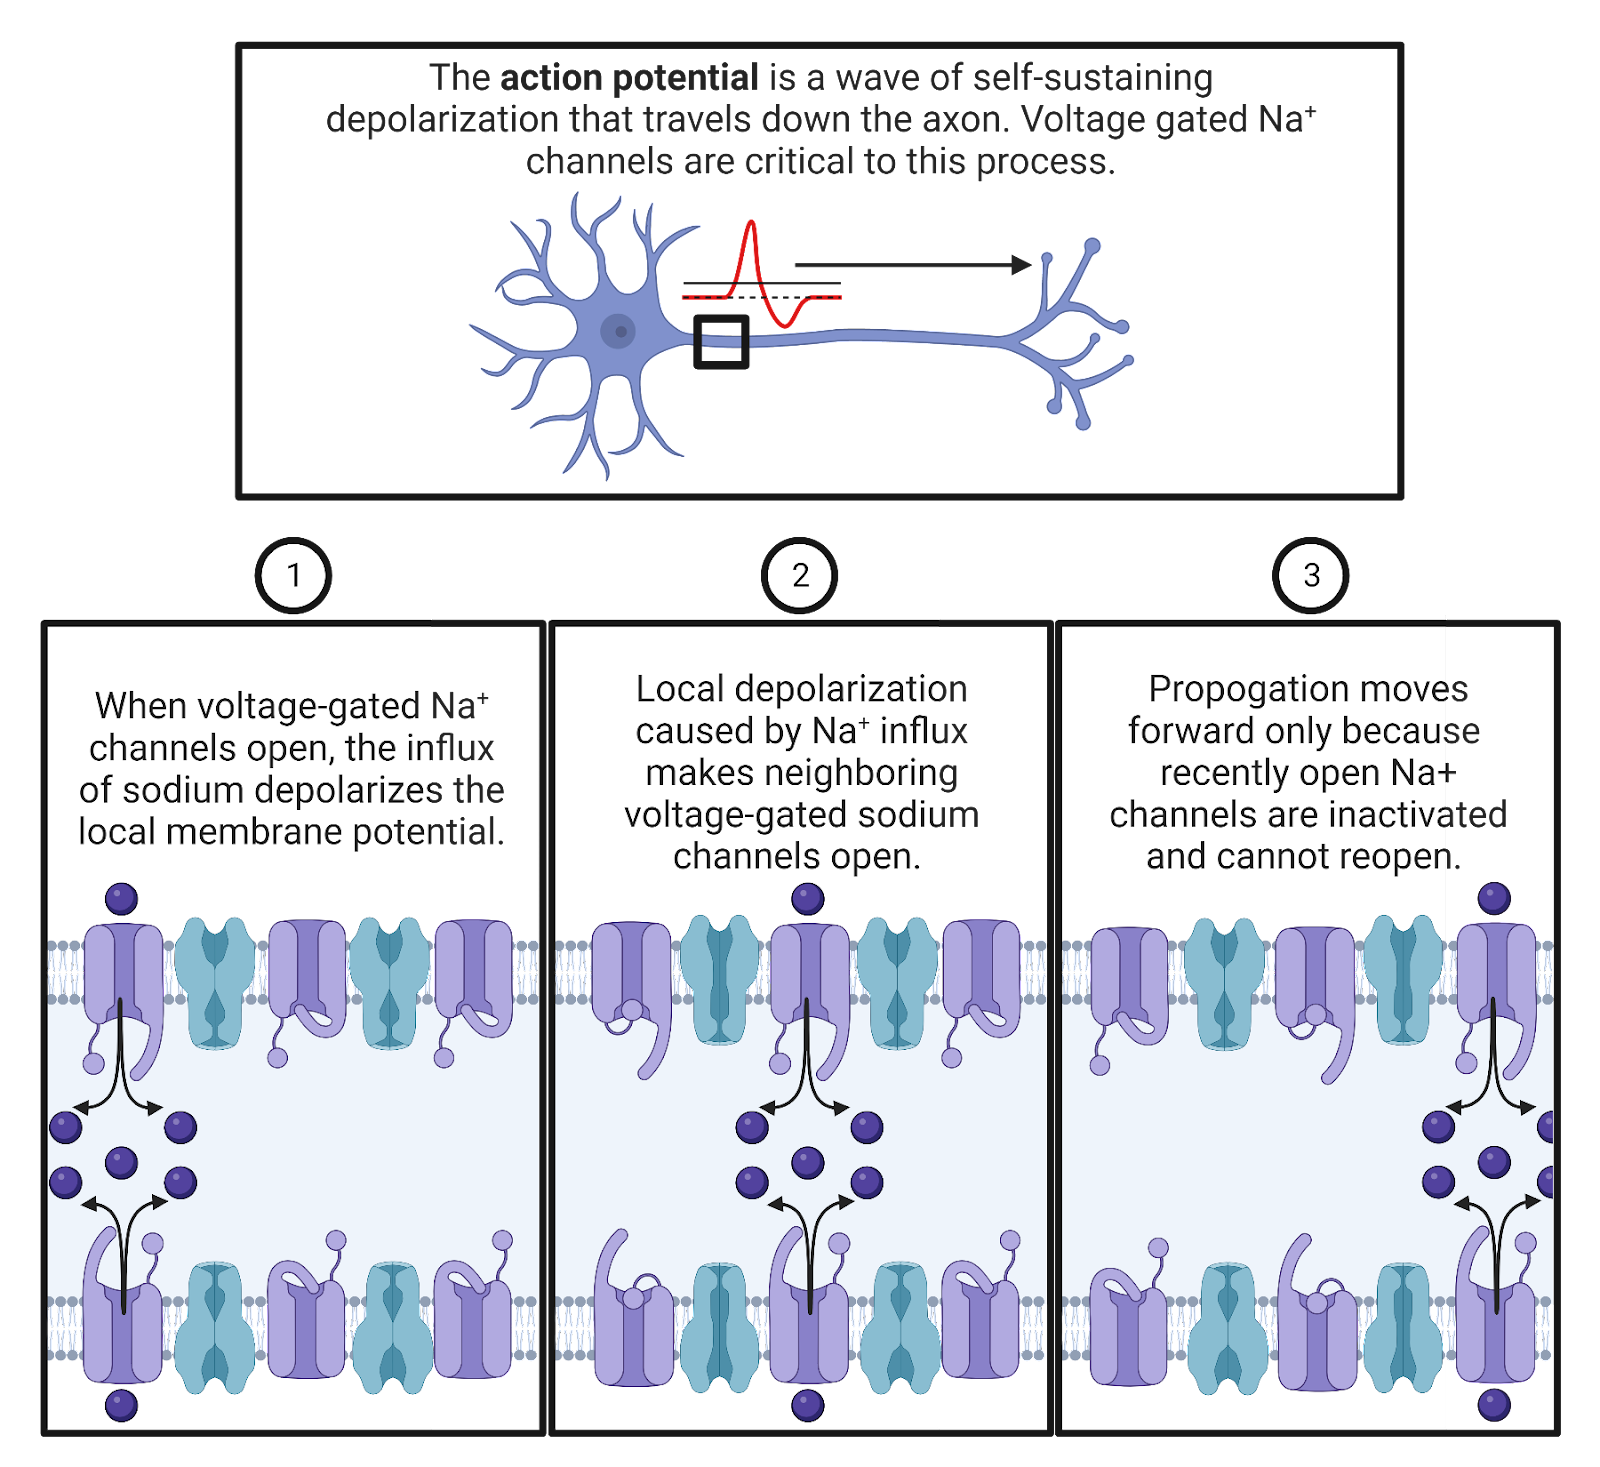
\includegraphics[width=0.8\linewidth]{images/ch02/02_26} 

}

\caption{Stay tuned!.}(\#fig:ch02_27)
\end{figure}

The falling phase is ``turbo charged'' by an additional channel: voltage-gated K+ channels. These channels are somewhat similar to the voltage-gated Na+ channels: they have a sensor that detects increases in the membrane potential, swiveling them open when there is sufficient excitation. When these channels are open, they provide additional conductance for K+ above and beyond what is provided by the leak K+ channels. This allows K+ to be more rapidly pushed out of the neuron by diffusion, accelerating the falling phase. You can think of K+ as soccer fans trying to leave a stadium after a match. Everyone could be anxious to leave, but if there are only a few exits it will take a long time for the stadium to empty. The opening of the voltage-gated K+ channels is like adding a bunch of new exits to the stadium, allowing a much more rapid departure of the crowd. Without the voltage-gated K+ channels, it would take a typical neuron about 2-3 times as long to return to rest after an action potential, and that would greatly limit the frequency at which neurons can send messages.

Although the voltage-gated K+ channels respond to excitation in the same way that Na+ channels do, they are different in two key ways. First, the K+ channels do not inactivate---they stay open as long as the neuron has a positive charge, working continuously to help the K+ battery charge the neuron back down to its negative resting potential. A second distinctive feature is that the voltage-gated K+ channels are \emph{slow}---their voltage sensor takes longer to open and to close the channels than the sensor on the voltage-gated Na+ channels. This ``tardiness'' is important, causing the K+ channels to only begin opening just as the Na+ channels are beginning to clog. This remarkable feat of timing makes the action potential extremely efficient, limiting the overlap between the increases in Na+ and K+ conductance that happen during the rising and falling phase. If the K+ channels opened earlier, K+ would be able to diffuse out of the neuron as quickly as the voltage-gated Na+ channels were allowing Na+ to diffuse in, an offsetting current that would produce no signal in the membrane potential!

A second consequence of the slow operation of the voltage-gated K+ channels is the undershoot. Even after the neuron begins to return to a negative charge, it takes a few milliseconds for the K+ channels to swivel closed. During this time, the combination of the leak K+ channels \emph{and} the voltage-gated K+ channels means that the K+ battery is even more in control in its ``tug of war'' with the Na+ battery, and can charge the neuron even closer to EK. We observe this as the neuron's membrane potential temporarily becoming even more negative than usual. As the voltage-gated K+ channels gradually close, the typical balance between K+ and Na+ leak conductances is restored, and the membrane returns to its typical resting membrane potential, slightly above EK.. This undershoot, like the clogging of the voltage-gated Na+ channels, helps limit excess activity.

\hypertarget{action-potential-propagation-is-sped-up-by-myelin.}{%
\subsection{Action potential propagation is sped up by myelin.}\label{action-potential-propagation-is-sped-up-by-myelin.}}

When you connect a battery to a wire, it pushes current directly through the circuit. As long as the wire is properly insulated, almost no current leaks out as it travels, so you don't need additional batteries along the length of the wire, and current covers the distance of the circuit at very close to the speed of light. That's why flipping a light switch instantly turns on your lights, even though the power station might be located several miles away.

As we have seen, that's not exactly how an action potential propagates. Instead, neuronal axons are ``leaky'', expressing leak K+ channels (as well as a lesser quantity of leak Na+ channels). This means that when the first segment of an axon experiences the rising phase, the Na+ that rushes can quickly be offset by K+ rushing out. Due to this leak, the action potential is \emph{regenerated} down the length of the axon, with each segment undergoing the precise opening and closing of voltage-gated channels that triggers the next segment, and so on. This takes time, and it means that the action potential does not travel down the axon at anything near the speed of light.

Many animals, including all mammals, have evolved ways to speed up action potential propagation by having support cells wrap axons in \emph{myelin}, a fatty substance that insulates the axon, greatly limiting the operation of the leak channels (Image 2.28). A segment of axon wrapped in myelin works more like the wires we're used to dealing with in electronics: a current applied to one end can spread rapidly, at almost the speed of light, with \_fairly \_little leakage. That's a great speedup in the spread of an action potential. Unfortunately, myelin isn't perfect, and there is still some leakage, so it can only effectively deliver currents over relatively short distances, around 1mm. Because of this, myelin is wrapped around axons in bands and between these bands are \textbf{nodes of Ranvier}, bare patches of axon crowded with voltage-gated channels that can regenerate the action potential and push current through the next band of myelin (the name comes from the French scientist, Louis Ranvier, who was one of the first to scientifically study myelin). The mix of relatively slow regeneration (at each node of Ranvier) and exceptionally fast current spread (through each segment of myelin) is called \textbf{saltatory conduction}, and it lets action potentials travel fast, at speeds of up to 150 meters per second (333 miles per hour). That's very slow compared to the currents in your cell phone, which approach the speed of light (almost 300 million meters per second or 670 million miles per hour). But it's still much faster than action potentials can travel in bare, unmyelinated neurons, which typically ranges between 0.5 to 10 meters per second (1 to 22 miles per hour).

\begin{figure}

{\centering 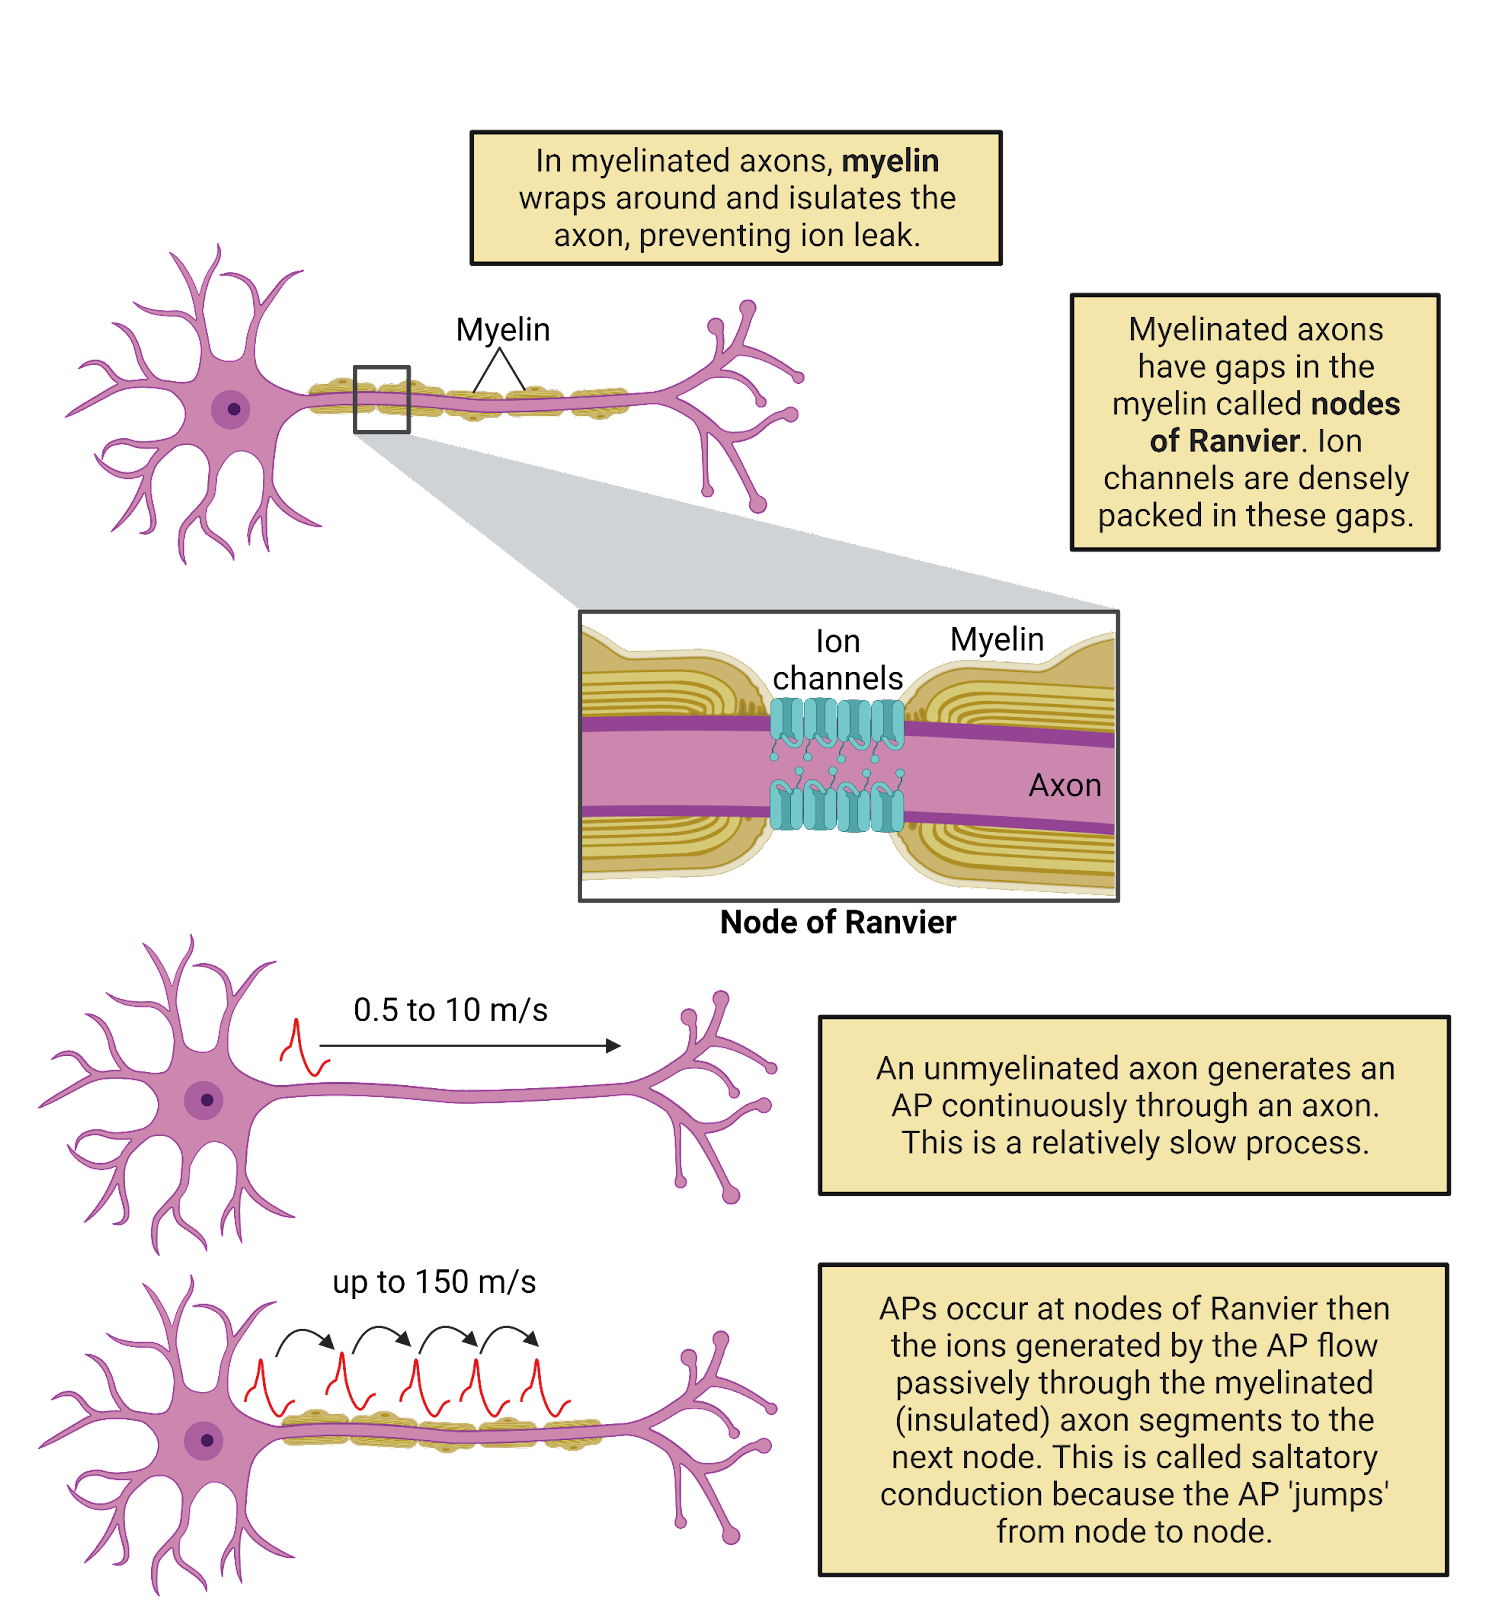
\includegraphics[width=0.8\linewidth]{images/ch02/02_27} 

}

\caption{Saltatory conduction.}(\#fig:ch02_28)
\end{figure}

Wrapping axons in myelin requires support cells and energy, so not all axons in the CNS are myelinated. But most \emph{tracts}, where axons from many neurons carry information over long distances do feature almost exclusively myelinated axons. The high density of fatty myelin in these tracts is what gives white matter its distinctive appearance.

\hypertarget{topic-summary-3}{%
\subsection{Topic summary}\label{topic-summary-3}}

Neural signaling represents an incredible ballet of electrolytes, pumps, and ion channels. The resting potential in neurons occurs due to moderate expression of leak K+ neurons and very limited expression of leak Na+ channels. These channels provide a constant strong conductance towards EK. (a negative potential) and a constant weak conductance towards ENa (a positive potential), a `tug of war' that causes neurons to exhibit and defend a resting potential a bit above EK, usually resting at around -65mV. Chemical messages from partner neurons disturb this rest, transiently binding to ligand-gated channels to produce post-synaptic potentials: small, transient local changes in membrane potential that push a neuron towards threshold (EPSP, due to Na+ or Ca++ conductance) or away from threshold (IPSP, due to Cl- conductance). When threshold is reached, an action potential is generated by a precisely timed sequence of Na+ entering through inactivating voltage-gated Na+ channels followed by K+ departure through voltage-gated K+ channels (Table 2.04).

\begin{figure}

{\centering 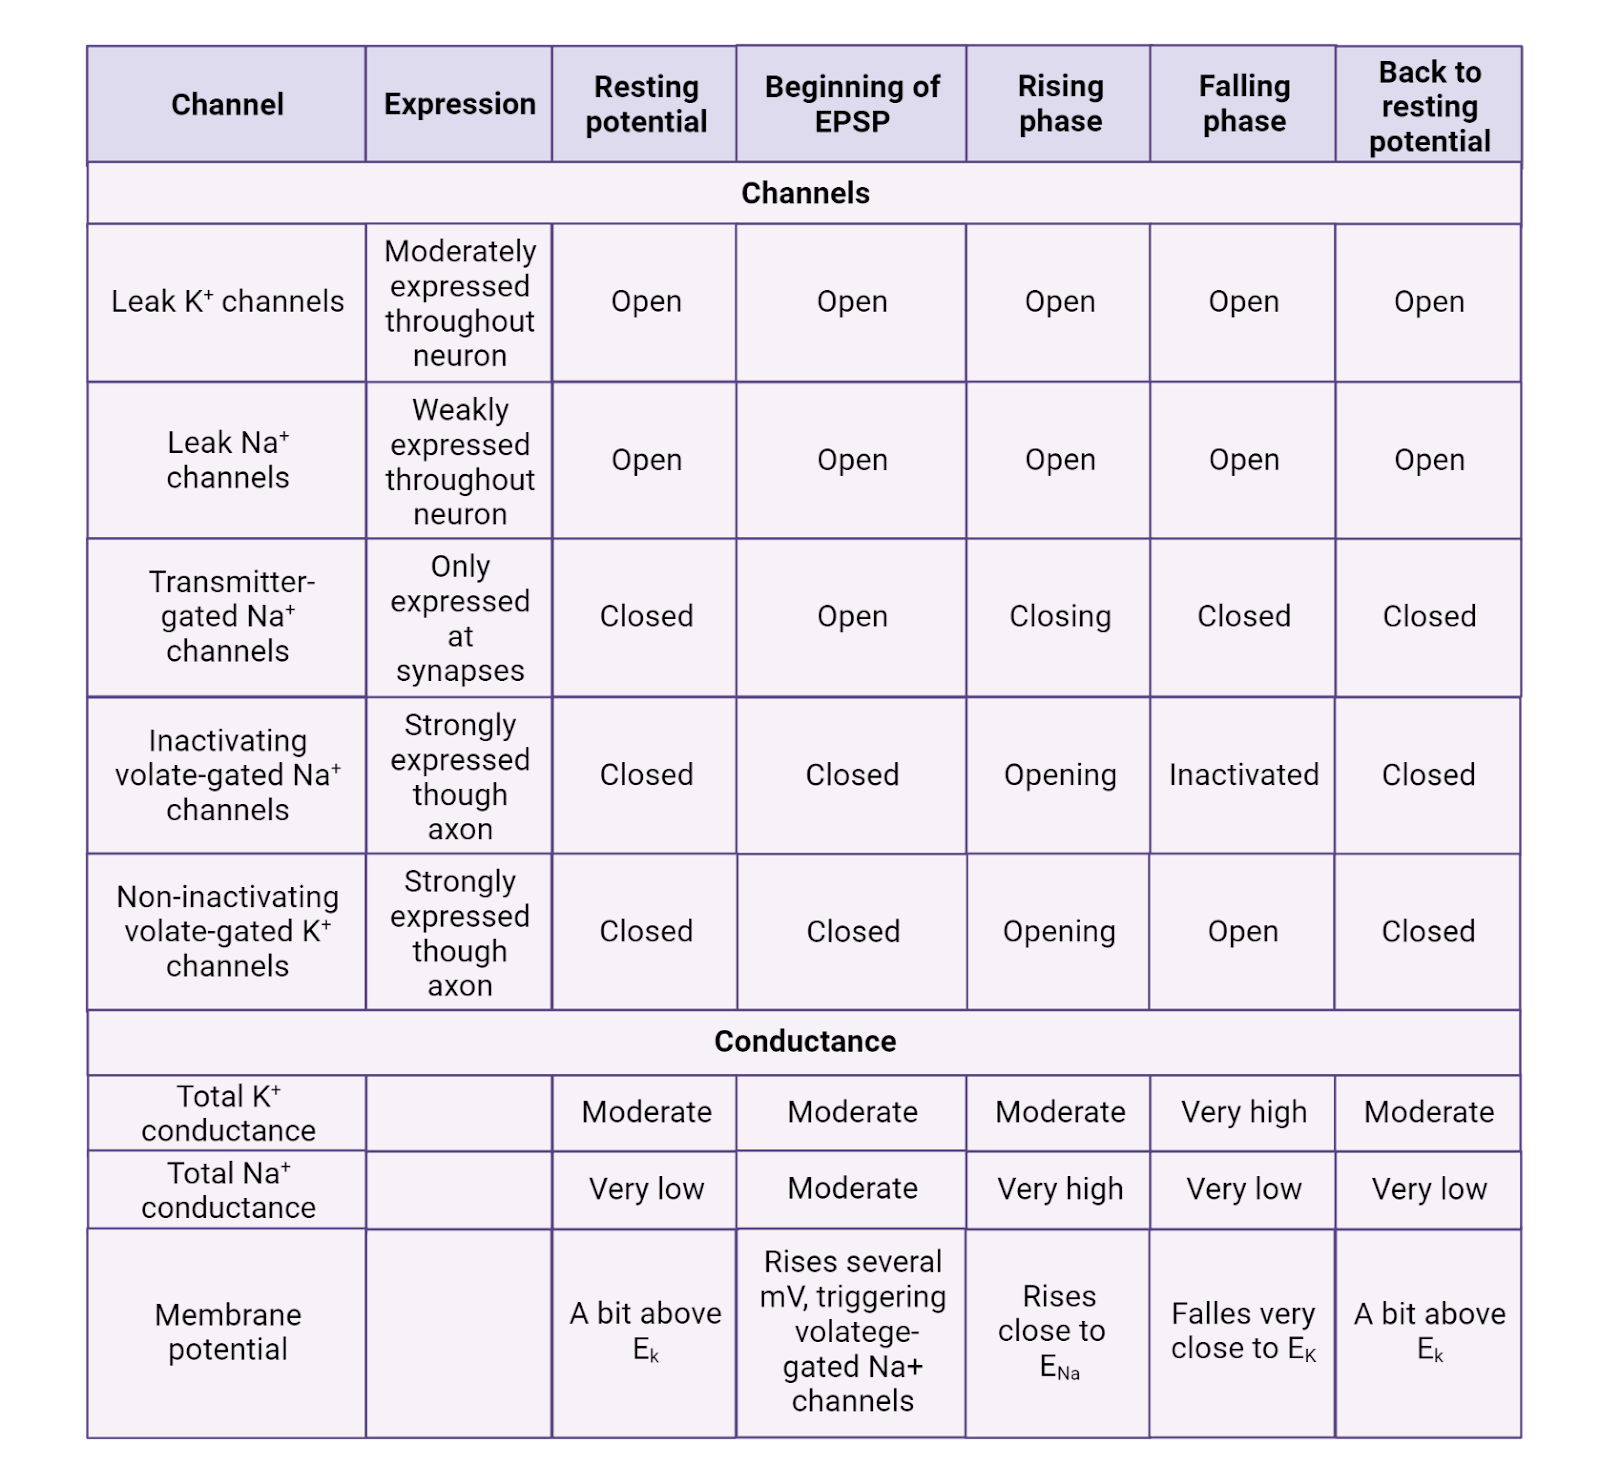
\includegraphics[width=0.8\linewidth]{images/ch02/table_02_04} 

}

\caption{Channels and conductances.}(\#fig:tbl_ch02_04)
\end{figure}

\textbf{Key Terms}

Resting potential

Leak K+ channels

Leak Na+ channels

Ligand-gated channel (aka Neurotransmitter-gated channel)

Action potential

Initial segment

Propagation

Rising phase

Falling phase

Undershoot

Inactivating voltage-gated Na+ channel

Voltage-gated K+ channel

Threshold

Positive feedback

Refractory period

\textbf{References and works cited}

\begin{itemize}
\item
  Eyal G, Verhoog MB, Testa-Silva G, Deitcher Y, Piccione RB, DeFelipe J, de Kock CPJ, Mansvelder HD, Segev I (2018) Human cortical pyramidal neurons: From spines to spikes via models. Front Cell Neurosci 12:1--24.
\item
  Viscardi LH, Imparato DO, Bortolini MC, Dalmolin RJS (2021) Ionotropic Receptors as a Driving Force behind Human Synapse Establishment. Mol Biol Evol 38:735--744.
\end{itemize}

\hypertarget{neurophysiology-wrapup}{%
\section{Our deep but still incomplete understanding of neural signaling}\label{neurophysiology-wrapup}}

\textbf{Learning objectives}

By the end of this section, students will be able to:

\begin{itemize}
\item
  Objective 1: Give examples of how our understanding of neural signaling has helped us understand specific medical conditions.
\item
  Objective 2: Describe some of the ways neural signaling is complex and still mysterious
\end{itemize}

This is a long and difficult chapter. That's because neuroscientists have succeeded in unraveling some of the important principles of neural communication. Moreover, what we covered was complex. Our understanding of neural signaling now ties together multiple levels of understanding, from physics (potential, current, and conductance), to chemistry (Na+, K+, Ca++, and Cl-), to biology (pumps, channels, membranes), providing a detailed and rich understanding of how neurons and their circuits \emph{process} information. Whew!

In this section, we'll tackle three topics. First, we'll examine the \emph{power} of understanding neural signaling, looking at examples of how that understanding has helped unravel long-standing medical mysteries. The last two sections provide some humble pie: first, by noting some of the additional complexity to neural signaling that was not discussed in this chapter, then by describing some of the many mysteries of neural signaling that still remain to be explored. Hopefully, this chapter will leave you with a sense of pride in your hard-won understanding of neural signaling and also with a sense of wonder for all there is left to learn.

\hypertarget{neuroscience-in-the-wild-neuroscience-helps-us-understand-dysfunctions-of-the-nervous-system}{%
\subsection{Neuroscience in the Wild: Neuroscience helps us understand dysfunctions of the nervous system}\label{neuroscience-in-the-wild-neuroscience-helps-us-understand-dysfunctions-of-the-nervous-system}}

Although getting your head around neural signaling can be exhausting, it is also rewarding, providing us with a powerful framework for understanding the function and dysfunction of the nervous system.

Think back to the beginning of this chapter @ref(\{neurophysiology-introduction\}), to Dr.~Q and his work to understand how a cancerous glioma can leave a patient with epilepsy even \emph{after} the glioma is removed. Dr.~Q's team has found that the uncontrolled growth of the glioma provokes surrounding neurons to increase their production of VGLUT1, a protein that helps load excitatory transmitter into synaptic vesicles. If you've made it through this chapter, you can now understand the excitement Dr.~Q's team when they made this discovery, and why they think it might explain the previously mysterious link between gliomas and seizures. If neurons make more VGLUT1, we should expect more excitatory transmitter loaded into each synaptic vesicle. That would mean more transmitter released for each action potential. \emph{That} should produce more activation of the ligand-gated Na+ channels that produce EPSPs, and that should mean larger EPSPs, letting each of the affected neurons be more likely to drive their partner neurons to fire action potentials, perhaps past the tipping point towards the runaway excitation that we observe as a seizure. That's still just a theory that will require much more exploration, but you can see how our understanding of neural signaling gives us a foothold for understanding (and possibly treating) dysfunctions of the nervous system.

Here are four more examples of how our understanding of neural signaling helps us better understand dysfunctions of the nervous system.

\textbf{Pumps and the resting membrane potential}. The \_``\_Poison Arrow Plant'' (\emph{Acokanthera schimperi}) found in eastern Africa contains a powerful toxin, ouabain, which causes heart arrhythmia, seizures, and, in strong enough doses, death (Image 2.29). The plant seems to produce this toxin as an adaptation to prevent animals from eating it. As the name of the plant suggests, though, the plant gained traditional uses making poison-tipped arrows, and there is even a species of African rat that anoints itself with the plant to protect itself! What makes ouabain so deadly? It turns out that it can bind to and stop ion pumps, especially those that maintain the high concentration of K+ inside a neuron. With the pumps stopped, the K+ concentration battery becomes progressively depleted. It is this concentration gradient in conjunction with the leak K+ channels that produces the resting potential, so as the concentration gradient for K+ fades, the resting potential becomes less and less negative, meaning that neurons are now ``resting'' ever closer to threshold (Miura and Rosen, 1978). As you might imagine, this breakdown of the resting potential leads to the runaway excitation that manifests itself in seizures, and erratic heart rate, and \textbf{spastic paralysis }(paralysis due to muscles locking up).

\begin{figure}

{\centering 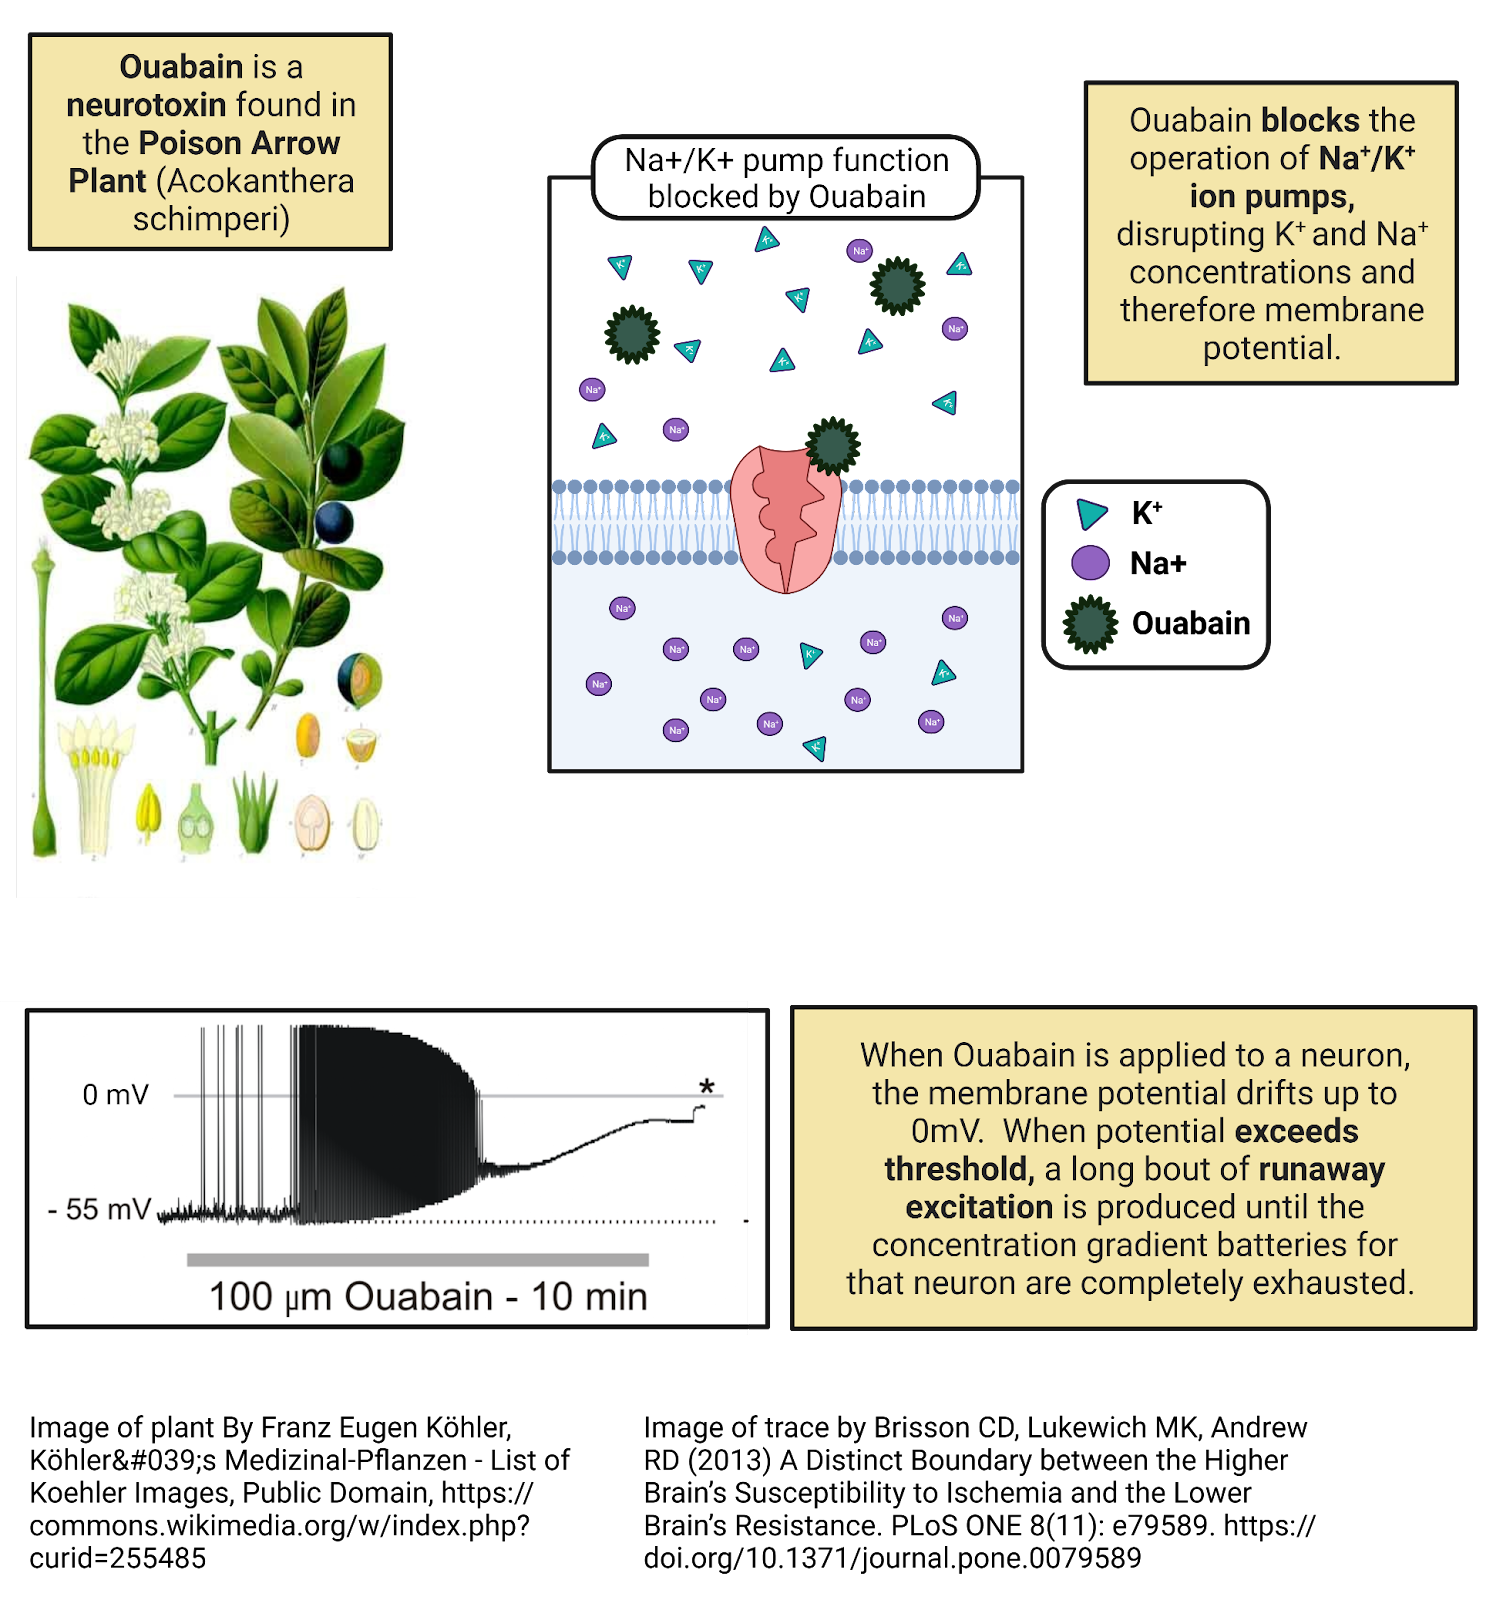
\includegraphics[width=0.8\linewidth]{images/ch02/02_28} 

}

\caption{Ouabain blocks Na+/K+ ion pumps.}(\#fig:ch02_29)
\end{figure}

\textbf{Ligand Gated Ion Channels and Post-Synaptic Potentials. }Childhood absence epilepsy is a form of epilepsy that emerges early in life (4-8 years) and is associated with frequent staring spells (Image 2.30). While this frequent ``absence'' from paying attention or responding to the outside world was once blamed on the child, each staring spell is actually a small-scale seizure. Genetic sequencing has shown that childhood absence epilepsy is often related to genetic mutations in one of the genes coding for a ligand-gated Cl- channel, a type of channel that normally helps produce IPSPs (Hirose, 2014). The most common disease-causing mutation is one that alters a special ``tag'' that helps target the channel to the neuronal membrane. With the mutated tag, the channels are manufactured by ribosomes, but remain in the cytoplasm, where they cannot detect transmitter from partner neurons and cannot generate IPSPs. It is this impairment of inhibition that likely leads to the runaway excitation that manifests as seizures. While childhood absence epilepsy can usually be treated with drugs that boost inhibition, most children grow out of this condition over time, a happy reminder that nervous systems can often adapt to maintain a proper balance of inhibition and excitation.

\begin{figure}

{\centering 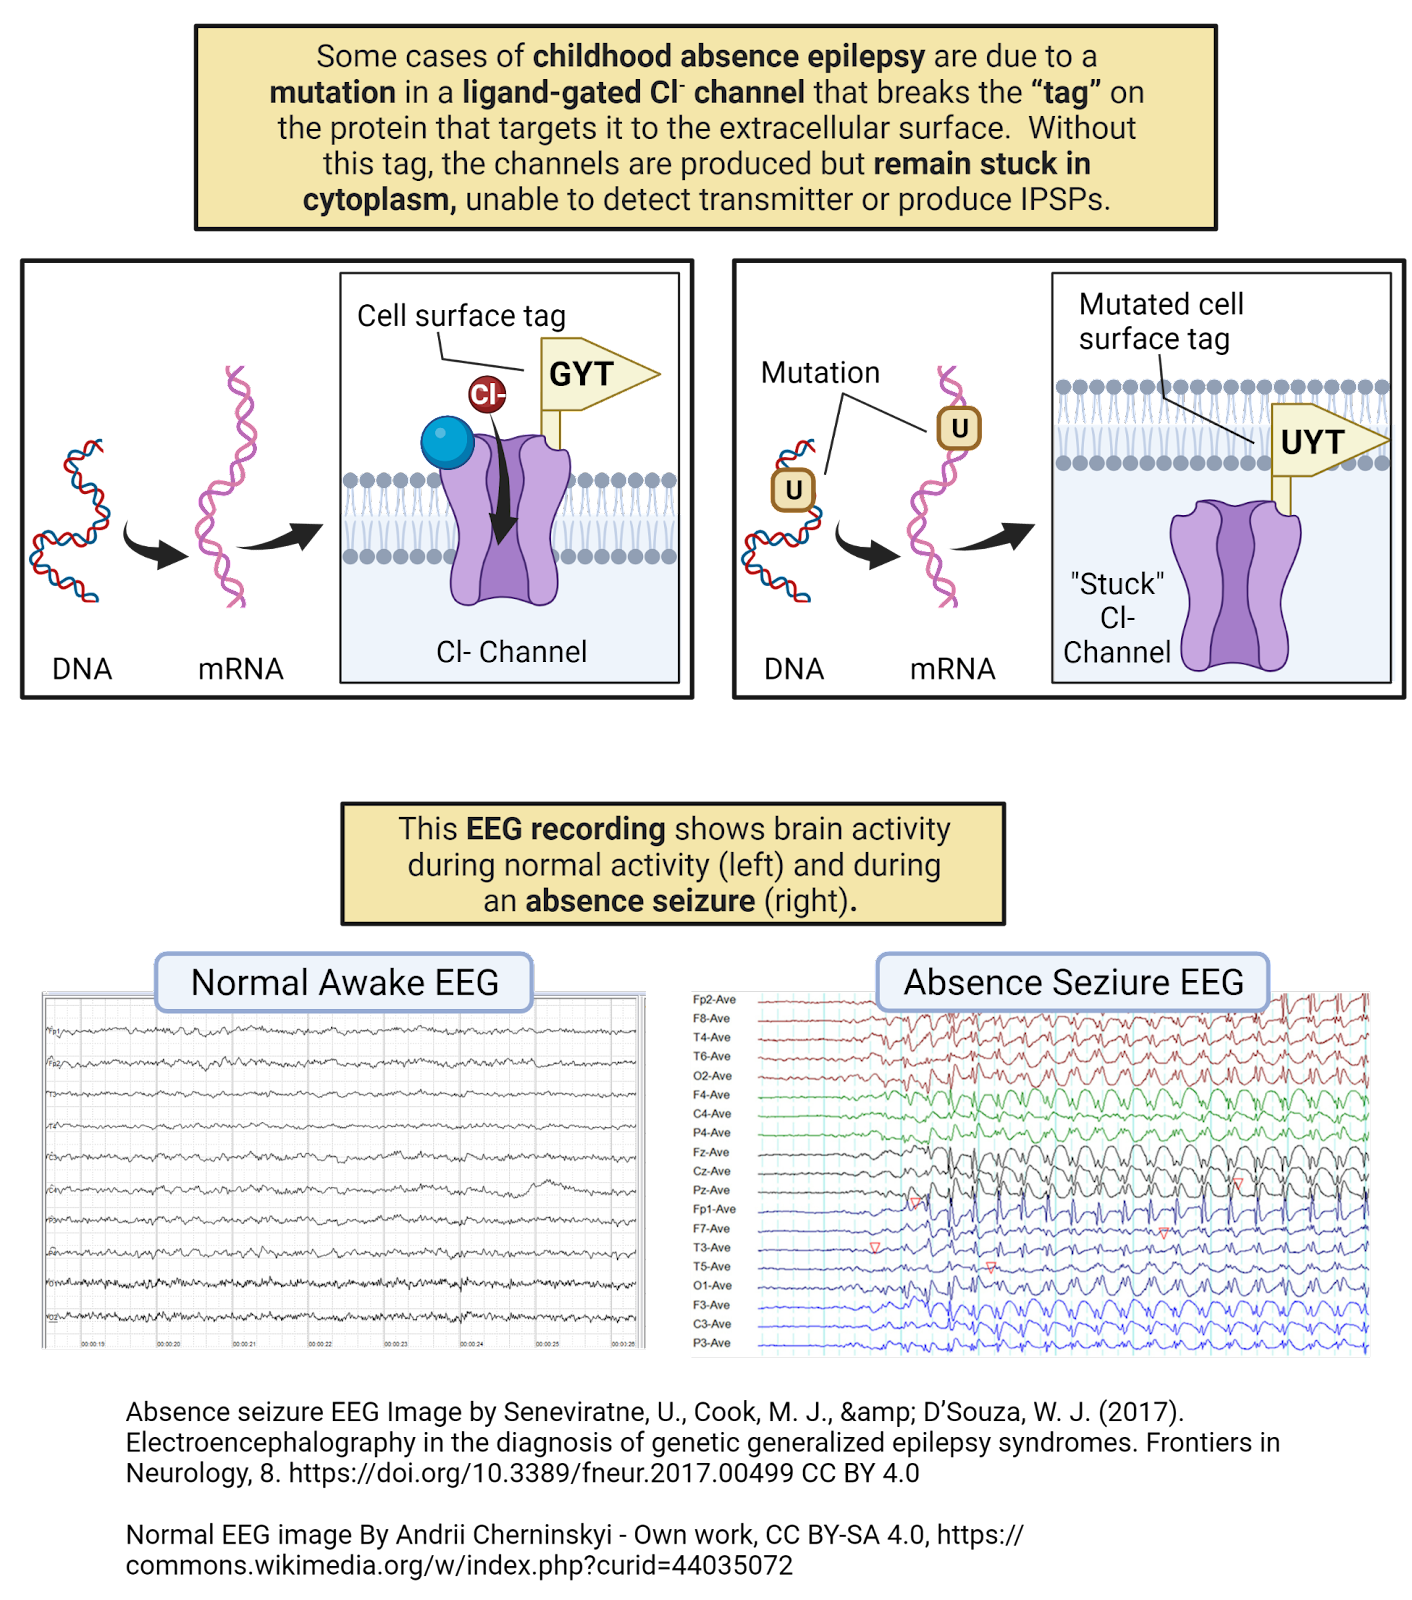
\includegraphics[width=0.8\linewidth]{images/ch02/02_29} 

}

\caption{Childhood absence epilepsy and mutations in ligand-gated Cl- channels.}(\#fig:ch02_30)
\end{figure}

\textbf{The Inactivating Voltage-gated Na+ Channels and the Action Potential}. Puffer fish (fish from the family \emph{Tetraodontidae}) are adorable, but most are highly toxic (Image 2.31). Why? Because of a symbiotic relationship puffer fish have evolved with special strains of bacteria in the \emph{Aremonas} family (Noguchi, 2008). Through a pathway that remains mysterious, puffer fish collaborate with these bacteria to produce tetrodotoxin (TTX), a neurotoxin that clogs the inactivating voltage-gated Na+ channels responsible for the rising phase of an action potential. In humans, ingestion of TTX causes tingling sensations as it initially shuts down signals from peripheral touch and pain receptors; it then shuts down motor neurons, causing \textbf{flaccid paralysis }(loss of muscle tone), coma, and the cessation of breathing function. Although deadly, TTX does not easily cross the blood-brain barrier, so those affected can remain lucid and aware even as the poison shuts down their body functions (!). Puffer fish are not the only animals who have evolved uses for TTX: it is the toxin injected by the bite of the dangerous blue-ringed octopus and it is also secreted in the skin of several species of poisonous amphibians. In fact, TTX is common enough in the animal kingdom that some predators have evolved counter-measures. For example, garter snakes have inactivating voltage-gated Na+ channels that are \emph{not} clogged by TTX, allowing them to dine on poisonous newts and frogs with impunity. For humans, though, TTX is one of the most toxic substances known, with even a milligram dose sufficient to cause death. Despite this, pufferfish is considered a delicacy in Japan, Korea, and parts of China where it is prepared by chefs specially trained in the removal of the toxic organs from the fish. While this special preparation is usually successful in removing almost all the TTX, rare cases of poisoning do occur. With no antidote available, the consumption of puffer fish can be considered a sort of culinary roulette; the real but low-probability danger is thought to heighten the dining experience.

\begin{figure}

{\centering 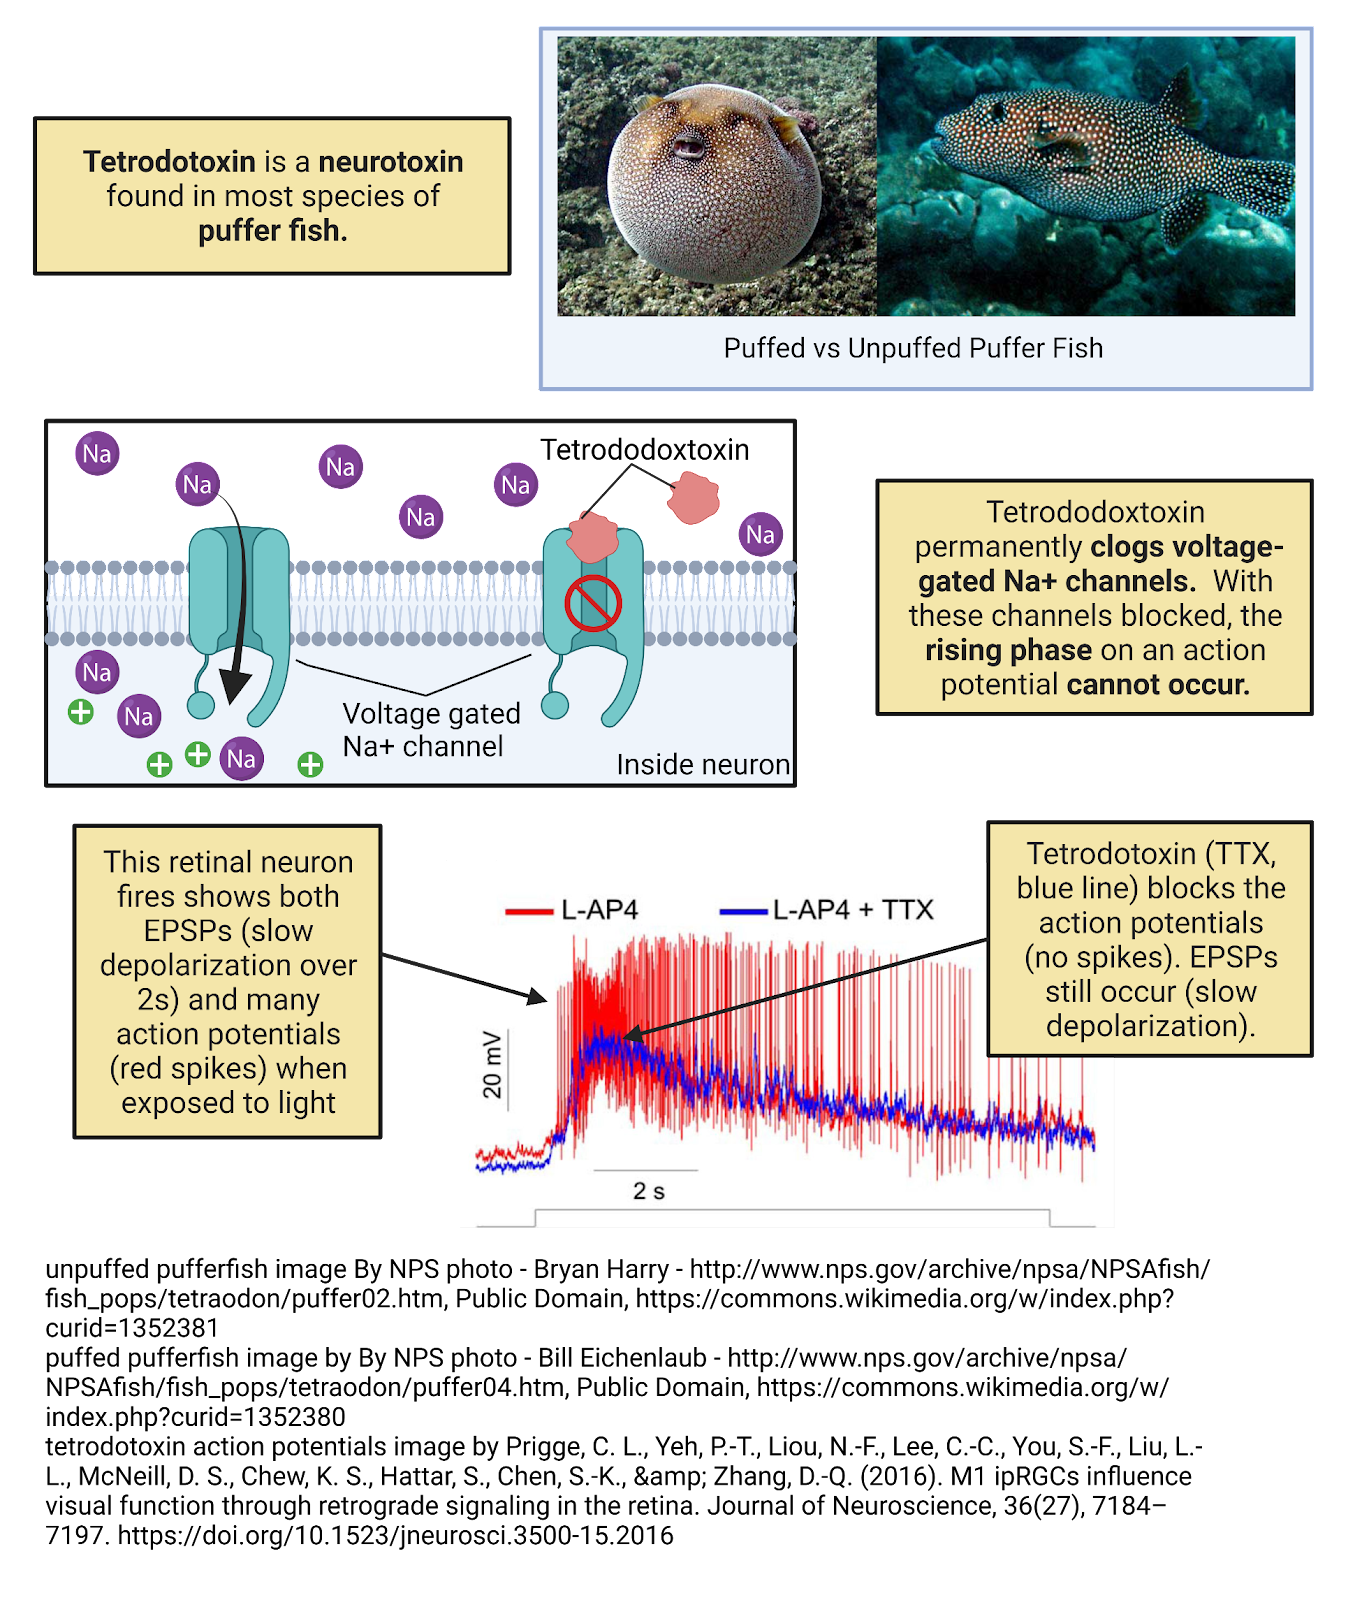
\includegraphics[width=0.8\linewidth]{images/ch02/02_30} 

}

\caption{Puffer fish poison.}(\#fig:ch02_31)
\end{figure}

\textbf{Myelin and Action Potential Propagation. }Multiple sclerosis (MS) is an \textbf{autoimmune disorder} affecting several million people worldwide (Image 2.32), especially women (who develop MS at a rate twice as high as men). The most common symptoms are episodes of muscle weakness, blurred vision, and/or changes in the sense of touch, including numbness, pins and needles, and tingling. The severity of MS varies among patients and can be fatal. We now know that MS is caused, in part, by the immune system attacking and destroying myelin. This causes inflammation of myelinated axons, loss of myelin, and even neuronal death, leaving behind lesions in the white matter of the nervous system (these lesions, often called \emph{sclerae}, formed the basis for naming the disease). We still don't understand why the immune system mis-recognizes myelin as something to attack in MS patients, nor why this comes and goes in distinctive episodes. But knowing that MS affects myelin explains a lot about its symptoms, since the most prominent white-matter tracts in the CNS are the cortico-spinal tract that sends motor commands from the cortex down to motor neurons in the spine and the somatosensory tracts bringing touch information from all over the body up the spine to the brain.

\begin{figure}

{\centering 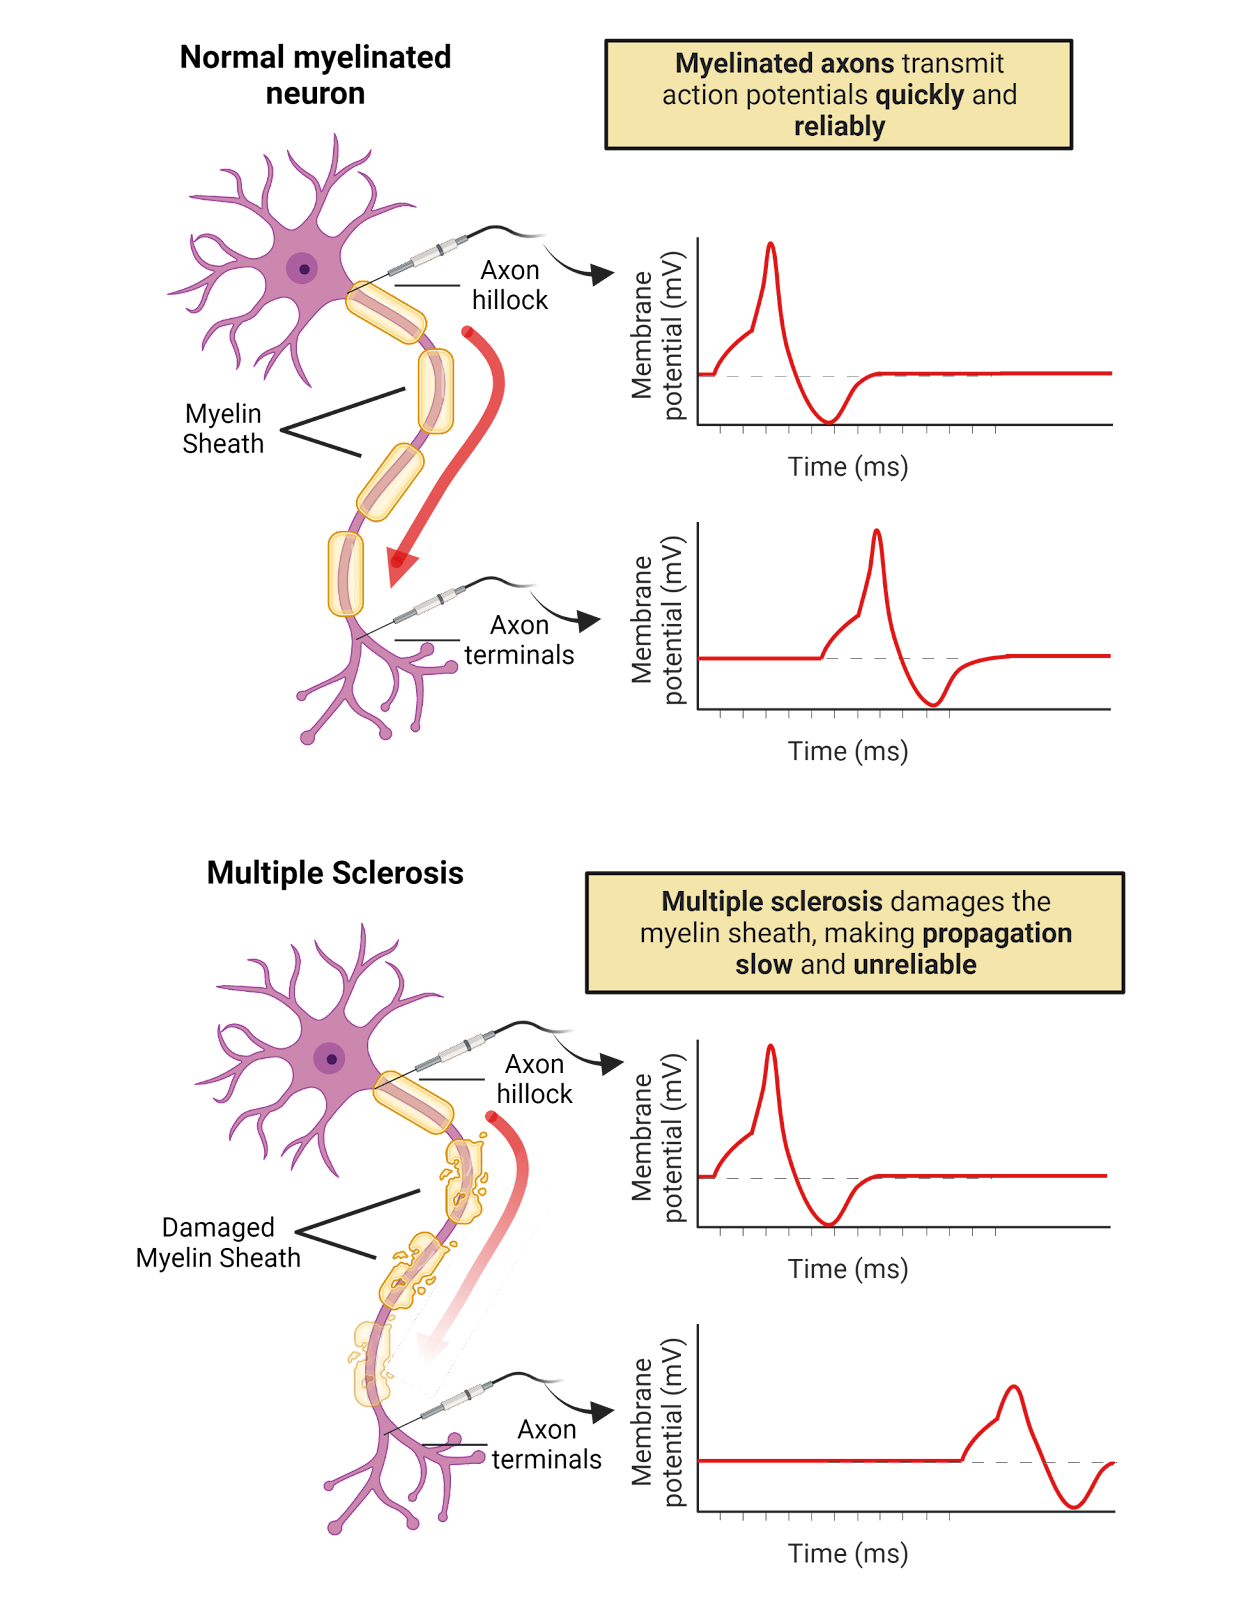
\includegraphics[width=0.8\linewidth]{images/ch02/02_31} 

}

\caption{Multiple sclerosis.}(\#fig:ch02_32)
\end{figure}

\hypertarget{neural-signaling-is-complex}{%
\subsection{Neural signaling is complex}\label{neural-signaling-is-complex}}

While we can feel triumph at the way neuroscience is helping to illuminate medical mysteries, it is important to note that this chapter only scratches the surface of what neuroscientists have discovered about neural signaling. For both space and clarity, some topics have been greatly simplified. That's fine: we needed to start somewhere, and this chapter was already quite long and complicated, right? But it's worth at least a peak behind the curtain at some of the additional complexities of neural signaling:

\begin{itemize}
\tightlist
\item
  \textbf{Chemical synapses are not only one-way}. In this chapter we've emphasized communication from the pre-synaptic to the post-synaptic neuron, noting that the pre-synaptic neuron is loaded with vesicles of transmitter to send messages and the post-synaptic membrane is studded with receptors to receive messages. It turns out this is only part of the story. The \emph{pre}-synaptic neuron also has receptors (often called \textbf{autoreceptors}) and the post-synaptic neuron releases messages back to the post-synaptic neuron (these are often called \textbf{retrograde messengers}). So while there are clear specializations for communication from pre- to post, it is more accurate to think of chemical synapses as a point of \emph{interaction} between neurons.
\item
  \textbf{Action potentials aren't always one-way either!} In this chapter we emphasized that action potentials are initiated at the initial segment of the axon and are then propagated down the axon. This is also just part of the story! In \emph{some} neurons action potentials also \textbf{backpropagate}, meaning that when they reach the end of the axon they then propagate \emph{back up the axon} to the cell body and sometimes also into the dendritic tree. In some experiments, blocking back-propagation has impaired plasticity, suggesting an important role in fine-tuning connectivity (Stuart et al., 1997).
\item
  \textbf{Synaptic messages are often quite complex. }We've explained how neurons release transmitter to partners to produce EPSPs (when binding to a ligand-gated Na+ channel), IPSPs (when binding to a ligand-gated Cl- channel), or neuromodulation (explained in Chapter on Neurochemistry). These are, indeed, the fundamental types of messages that can be communicated at chemical synapses. Things become more complex, however, when we realize that a pre-synaptic neuron can actually release multiple transmitters (called \textbf{co-transmitters}) and that the post-synaptic neuron can express multiple types of receptors. This means that what one neuron ``says'' to another at a chemical synapse can be very complex, often involving a blend of excitation, inhibition, and modulation!
\item
  \textbf{It's not just \emph{neural} signaling taking place in the nervous system; \emph{glia} are involved, too}. Glial have long been considered mere support cells in the nervous system, but there is increasing evidence that they play important roles in nervous system communication as well (Allen and Lyons, 2018). Glia express many different types of receptors, they can both absorb and release transmitters, and they exchange signals with neurons that seem to play important roles in determining which synapses a neuron forms and maintains.\\
\item
  \textbf{Neurons are astonishingly diverse}. This chapter has tried to describe signaling in a ``typical'' neuron. This leaves out the tremendous diversity of neurons. First, there is incredible variety across species. Not all species have myelin. Not all species have a clear distinction between dendrites and axons. In fact, some species even lack inactivating voltage-gated Na+ channels and instead have Ca++-based action potentials! Even within a species, there is incredible variety in size, shape, and signaling (Image 2.33).
\end{itemize}

\begin{figure}

{\centering 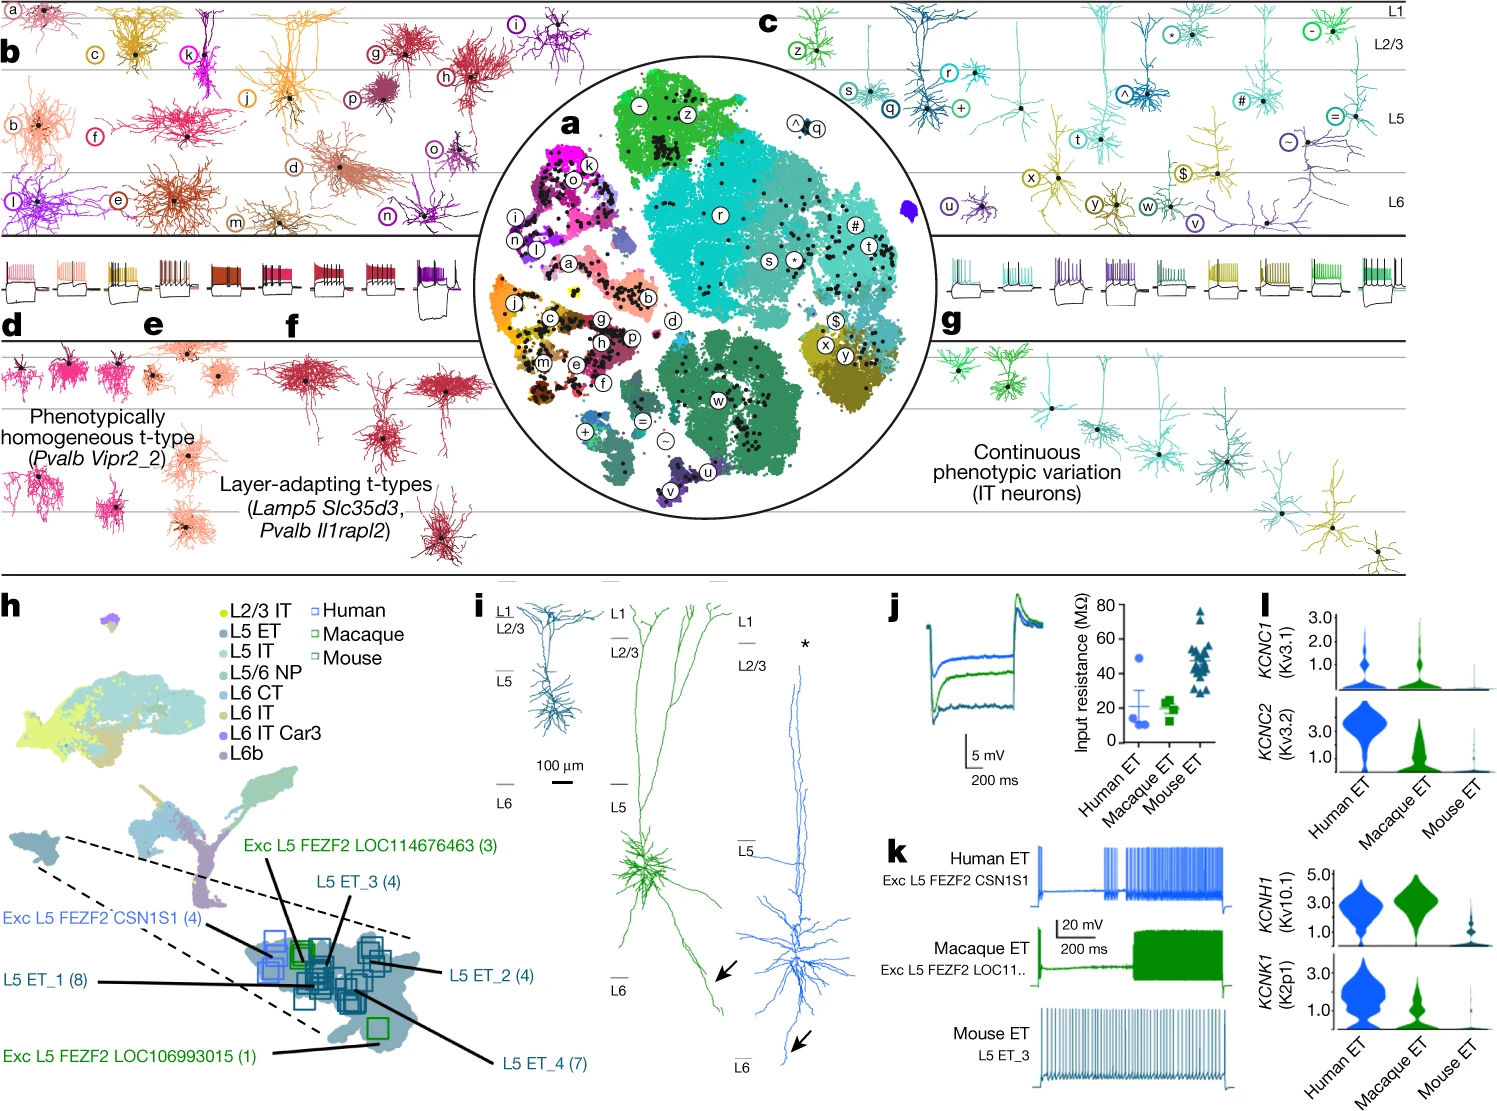
\includegraphics[width=0.8\linewidth]{images/ch02/02_32} 

}

\caption{Diversity in neurons -- FIGURE STILL IN DEVELOPMENT, STAY TUNED.}(\#fig:ch02_33)
\end{figure}

\hypertarget{there-is-still-so-much-to-learn-about-neural-signaling}{%
\subsection{There is still so much to learn about neural signaling}\label{there-is-still-so-much-to-learn-about-neural-signaling}}

We shouldn't leave this chapter with the impression that neuroscientists have figured it all out. There is still so much about neural signaling that we \emph{don't} know, and there is still tremendous promise for applying the bits we do know to improve our lives. So, let's end this difficult chapter by highlighting just a few of the many mysteries still to be resolved. That way we can close inspired by the possibility of helping to solve these mysteries, and with dreams of the better world we might build with that knowledge.

\begin{itemize}
\tightlist
\item
  \textbf{How do neuronal circuits maintain their function despite changing circumstances? } Most humans learn to walk early in life, at about 2 years of age. By adulthood, however, you are about twice as tall as you were when you learned to walk. That means the walking circuits in your spine have had to adapt throughout your lifetime. As you grew, the axons and dendrites in your walking circuits had to be extended over longer and longer distances. As your mass and center of gravity changed, inputs and outputs had to be adjusted to adapt the muscle commands for walking. Through it all, you experienced no major disruptions--you just kept on being able to walk! This is just one example of the \textbf{homeostasis }in neural circuits--their ability to maintain the same function despite tremendous change (Marder and Goaillard, 2006). We don't fully understand how this works (does each neuron have an `ideal' level of activity it is striving for?) or why some changes are easy for a neural circuit to cope with while others cause dysfunction.\\
\item
  \textbf{How do neuronal circuits self-organize? }Each of your neurons carries your entire genome, about 6.4 billion base-pairs of DNA. That's an impressive amount of DNA, but it is simply not enough DNA to provide a complete wiring diagram for each of the 86 billion neurons in your brain. And yet, most human brains end up with striking and recognizable similarities in organization, with axons of sensory neurons finding their way to the thalamus, axons of the primary motor cortex descending down to the lumbar spine, etc. How does the human brain self-assemble? And is the assembly program fixed or does it incorporate feedback from the developmental environment? The chapter on Neurodevelopment discusses in more depth what we know and don't know about the self-organization of neural circuits.
\item
  \textbf{How many types of neurons are in the human brain? }Neuroscientists have long sought to create a classification system for neurons: to develop a complete list of the different \emph{types} of neurons in the human brain (Bakken et al., 2021). While some differences seem clear (compare a cortical pyramidal neuron to spiny neuron in the basal ganglia), it has proven remarkably difficult to come up with a clear and consistent classification system. Molecular analysis has shown that two neurons that \emph{look} alike might express markedly different channels and transmitters. Meanwhile, neurons that look different can serve very similar functions. As an added layer of complication, neurons are constantly adapting to new circumstances, so what seems like one type of neuron might adapt over time in ways that make it very difficult to classify. Maybe we're not thinking about neuron identity correctly? Or maybe we just need to crunch more data to see the patterns? Or, perhaps, neurons are so adaptable that detailed typologies aren't possible. This is a sobering gap in our knowledge: despite all we do know about the human brain we still don't have a master parts list! There really is so much more to learn.
\end{itemize}

\hypertarget{topic-summary-4}{%
\subsection{Topic summary}\label{topic-summary-4}}

Neuroscientists have developed a rich and detailed understanding of neural signaling that is helping us better understand and treat disorders of the nervous system. While this progress is encouraging, there is a daunting level of complexity to nervous system function and many important mysteries left to unravel.

\textbf{Key Terms}

Autoimmune disorder

Autoreceptors

Backpropagate

Flaccid paralysis

Homeostasis

Retrograde messengers

Spastic paralysis

\textbf{References and works cited}

\begin{itemize}
\item
  Allen NJ, Lyons DA (2018) Glia as architects of central nervous system formation and function. Science (80- ) 362:181--185 Available at: \url{https://www.science.org/doi/10.1126/science.aat0473}.
\item
  Bakken TE et al.~(2021) Comparative cellular analysis of motor cortex in human, marmoset and mouse. Nature 598:111--119 Available at: \url{https://www.nature.com/articles/s41586-021-03465-8}.
\item
  Hirose S (2014) Mutant GABAA receptor subunits in genetic (idiopathic) epilepsy. In, pp 55--85 Available at: \url{https://linkinghub.elsevier.com/retrieve/pii/B978044463326200003X}.
\item
  Marder E, Goaillard J-M (2006) Variability, compensation and homeostasis in neuron and network function. Nat Rev Neurosci 7:563--574 Available at: \url{https://www.nature.com/articles/nrn1949}.
\item
  Miura DS, Rosen MR (1978) The effects of ouabain on the transmembrane potentials and intracellular potassium activity of canine cardiac Purkinje fibers. Circ Shock 42:333--338.
\item
  Noguchi T (2008) Tetrodotoxin -- Distribution and Accumulation in Aquatic Organisms, and Cases of Human Intoxication. Mar Drugs 6:220--242 Available at: \url{http://www.mdpi.org/marinedrugs/list08.htm\#10.3390_md20080011}.
\item
  Stuart G, Spruston N, Sakmann B, Häusser M (1997) Action potential initiation and backpropagation in neurons of the mammalian CNS. Trends Neurosci 20:125--131 Available at: \url{https://linkinghub.elsevier.com/retrieve/pii/S0166223696100758}.
\end{itemize}

  \bibliography{book.bib,packages.bib}

\end{document}
